\subsection{Correlations in the control region TT}
We present the correlations among variables in the control region TT in the figures \ref{fig:corrMatrix_CRTT} and
\ref{fig:correlations_CRTT_drbjets_S} and \ref{fig:correlations_CRTT_drbjets_BG}.

%\begin{center}
\begin{figure}[!htb]%hbpt?        
\centering

\includegraphics[width=0.65\textwidth]{figures/CRTT/dataset/plots/CorrelationMatrixS.pdf}
\bigbreak
\includegraphics[width=0.65\textwidth]{figures/CRTT/dataset/plots/CorrelationMatrixB.pdf}
%% \includegraphics[width=0.5\textwidth, height=0.2\textheight,  keepaspectratio]{figures/eles_bdt_vs_r/gr_limits__270GeV.pdf}
%% \includegraphics[width=0.5\textwidth, height=0.2\textheight,  keepaspectratio]{figures/eles_bdt_vs_r/gr_limits__300GeV.pdf}
%% \includegraphics[width=0.5\textwidth, height=0.2\textheight,  keepaspectratio]{figures/eles_bdt_vs_r/gr_limits__350GeV.pdf}
%% \includegraphics[width=0.5\textwidth, height=0.2\textheight,  keepaspectratio]{figures/eles_bdt_vs_r/gr_limits__400GeV.pdf}
%% \includegraphics[width=0.5\textwidth, height=0.2\textheight, keepaspectratio]{figures/eles_bdt_vs_r/gr_limits__450GeV.pdf}
%% \includegraphics[width=0.5\textwidth, height=0.2\textheight, keepaspectratio]{figures/eles_bdt_vs_r/gr_limits__600GeV.pdf}
%% \includegraphics[width=0.5\textwidth, height=0.2\textheight, keepaspectratio]{figures/eles_bdt_vs_r/gr_limits__650GeV.pdf}
%% \includegraphics[width=0.5\textwidth, height=0.2\textheight, keepaspectratio]{figures/eles_bdt_vs_r/gr_limits__900GeV.pdf}
%% \hspace{1.9cm}
%% \includegraphics[width=0.5\textwidth, height=0.2\textheight, keepaspectratio]{figures/eles_bdt_vs_r/gr_limits__1000GeV.pdf}
\caption{ Correlation matrices for the real data (denoted as signal) and background (mix of DY and TT) in the control region TT, in the names of few variables the index '1' refers to bb and the index '0' refers to ZZ}
\label{fig:corrMatrix_CRTT}                                                       
\end{figure}
%\end{center}





\begin{figure}[!htb]%hbpt?        
\centering
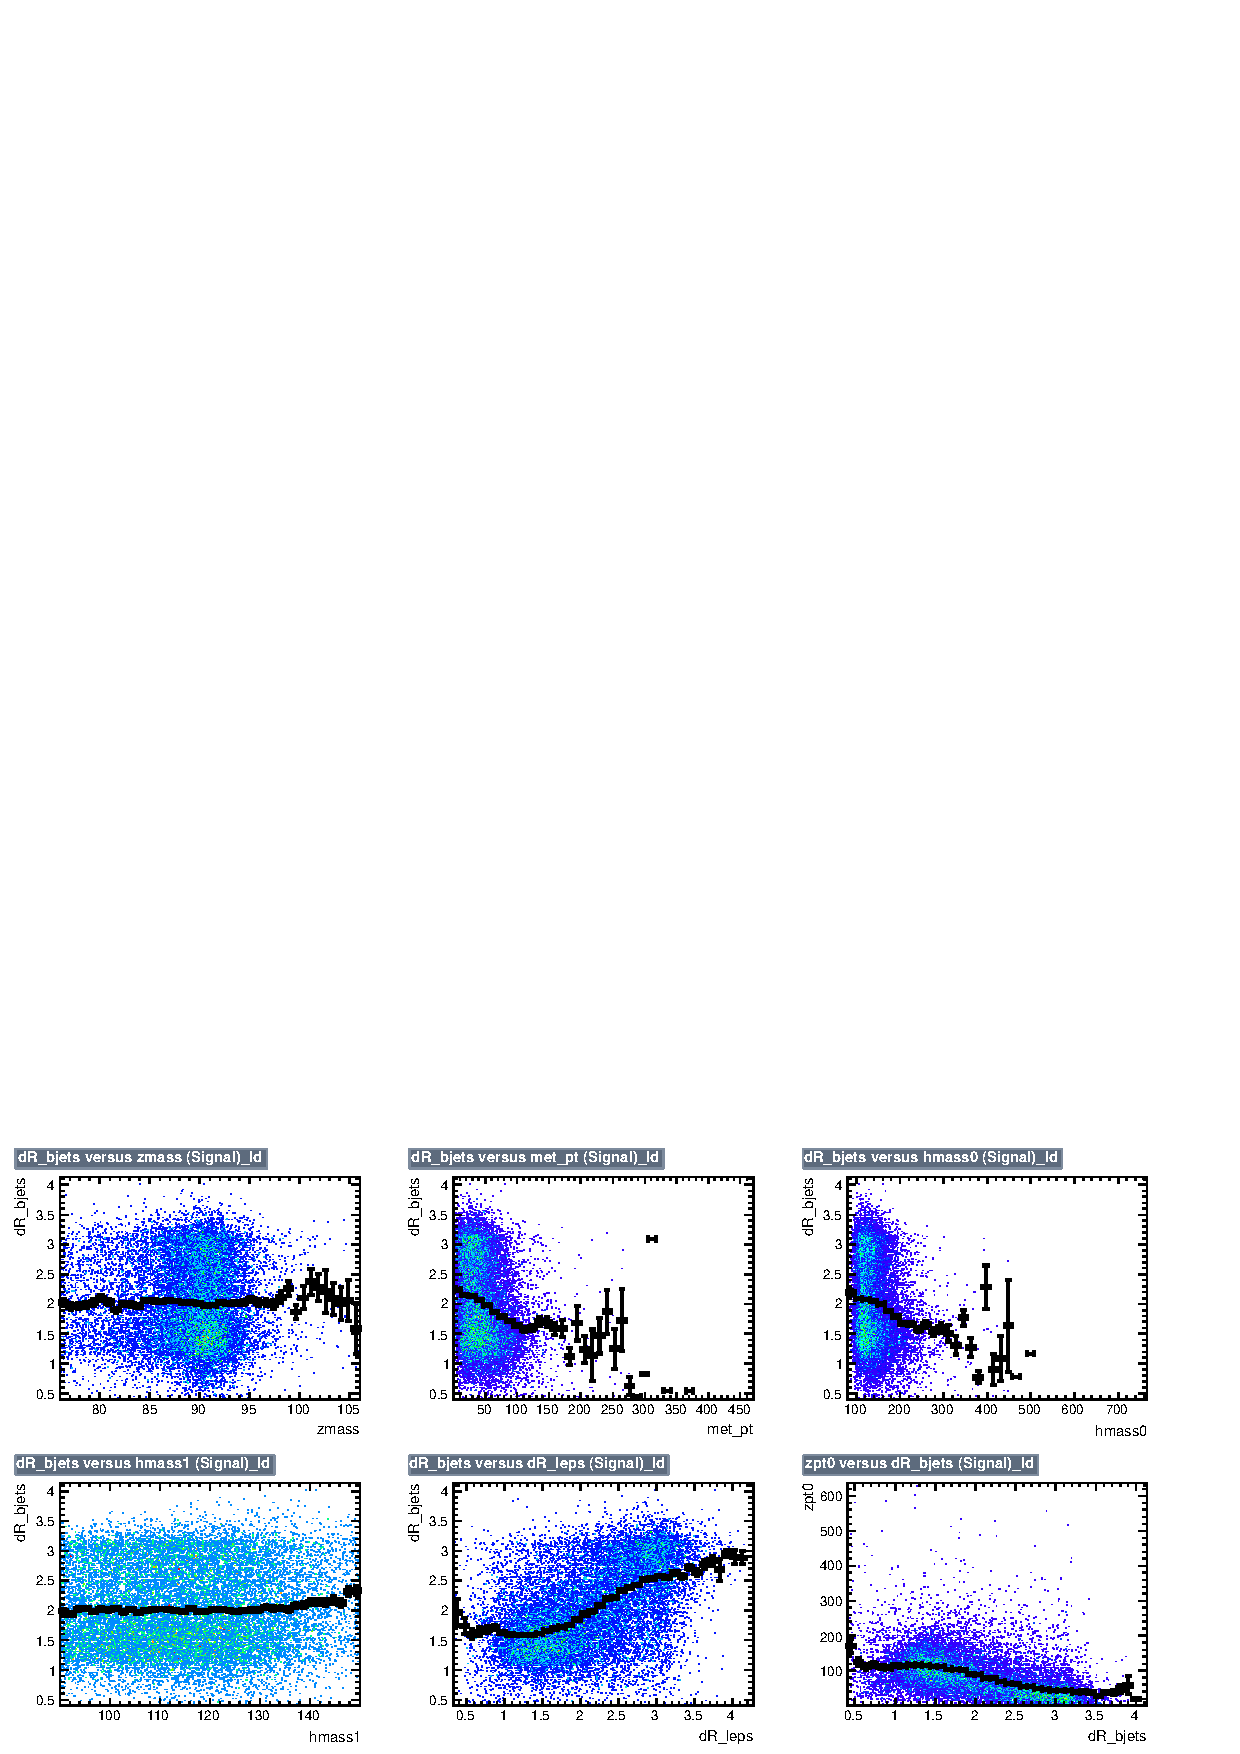
\includegraphics[width=0.95\textwidth]{figures/CRTT/dataset/plots/correlationscatter_dR_bjets__Id_c1.pdf}
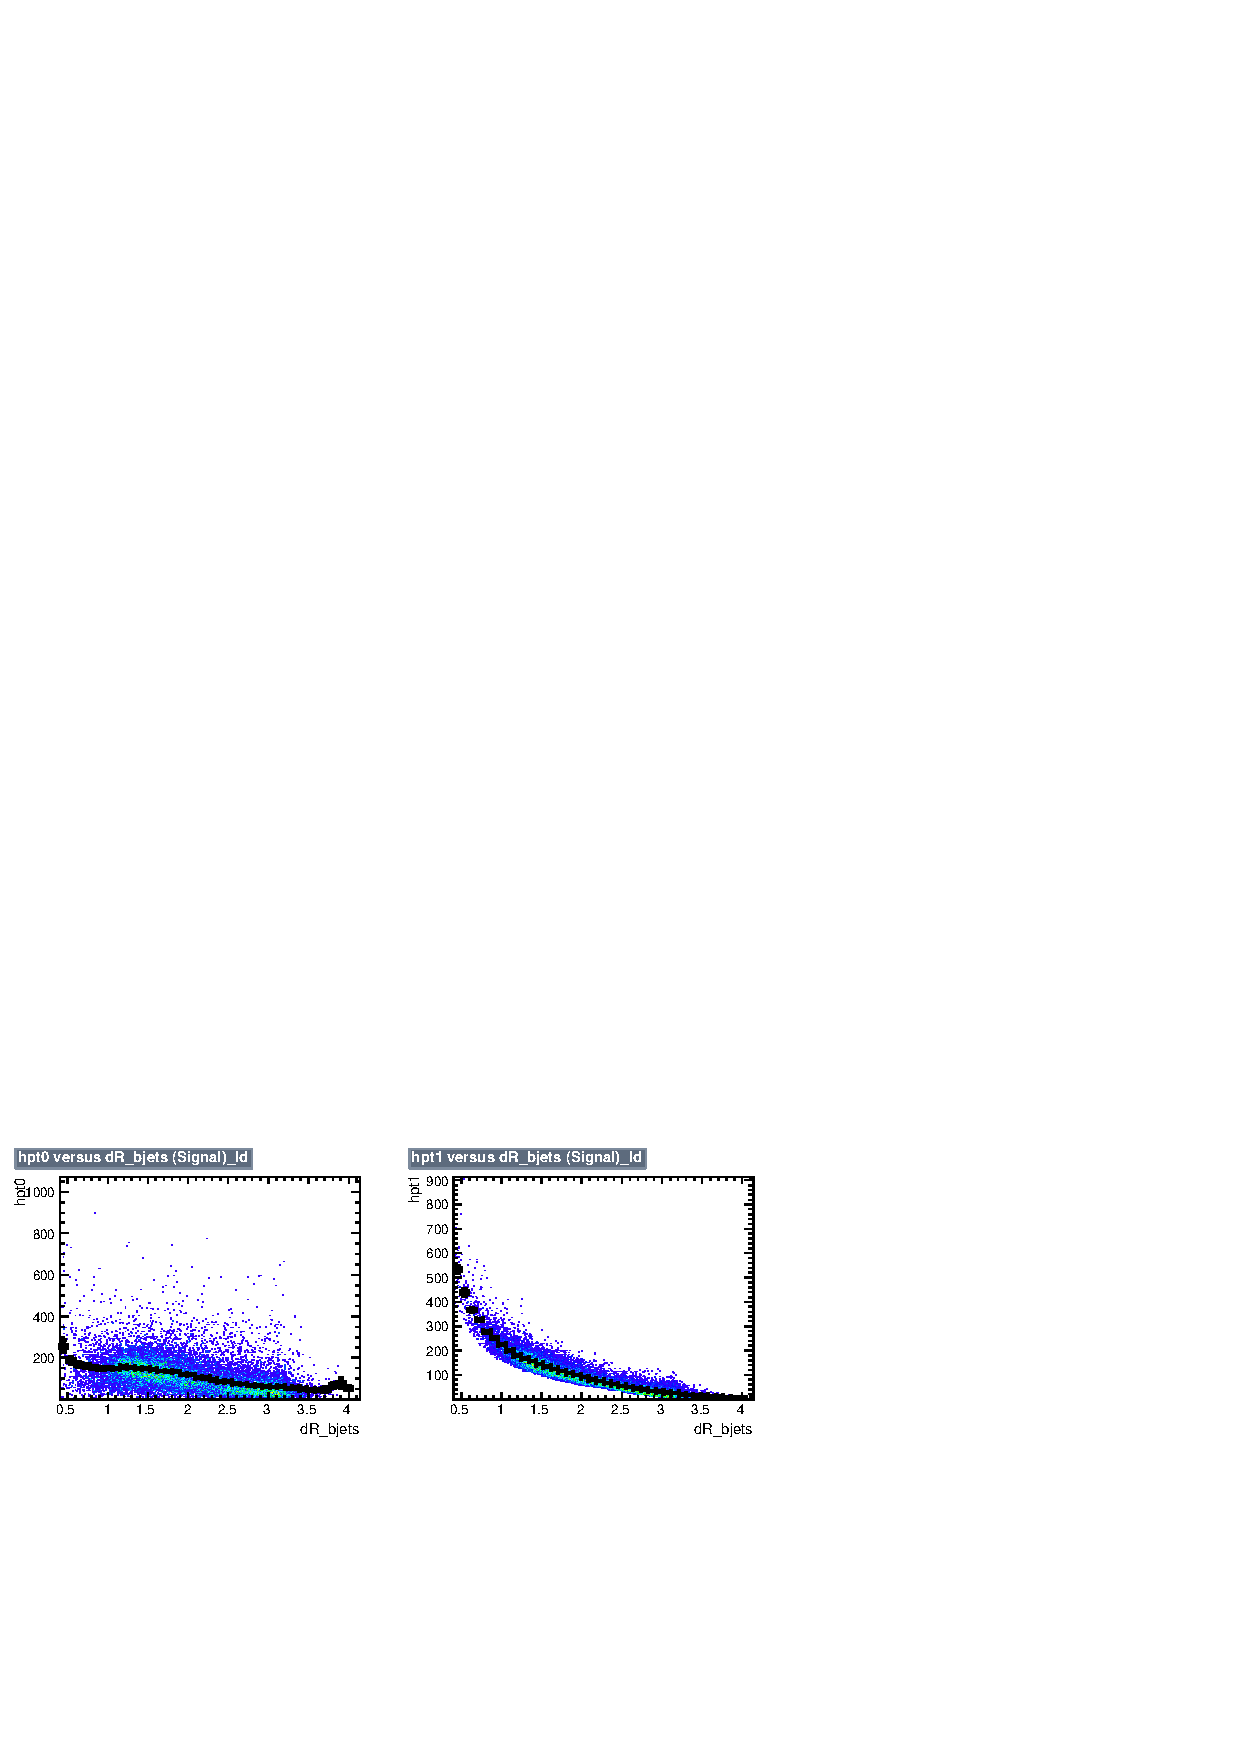
\includegraphics[width=0.95\textwidth]{figures/CRTT/dataset/plots/correlationscatter_dR_bjets__Id_c2.pdf}
\caption{ Correlation scatter plots for dR between bjets variable for data}%, index '1' refers to bb and index '0' refers to ZZ}
\label{fig:correlations_CRTT_drbjets_S}                                                       
\end{figure}



\begin{figure}[!htb]%hbpt?        
\centering
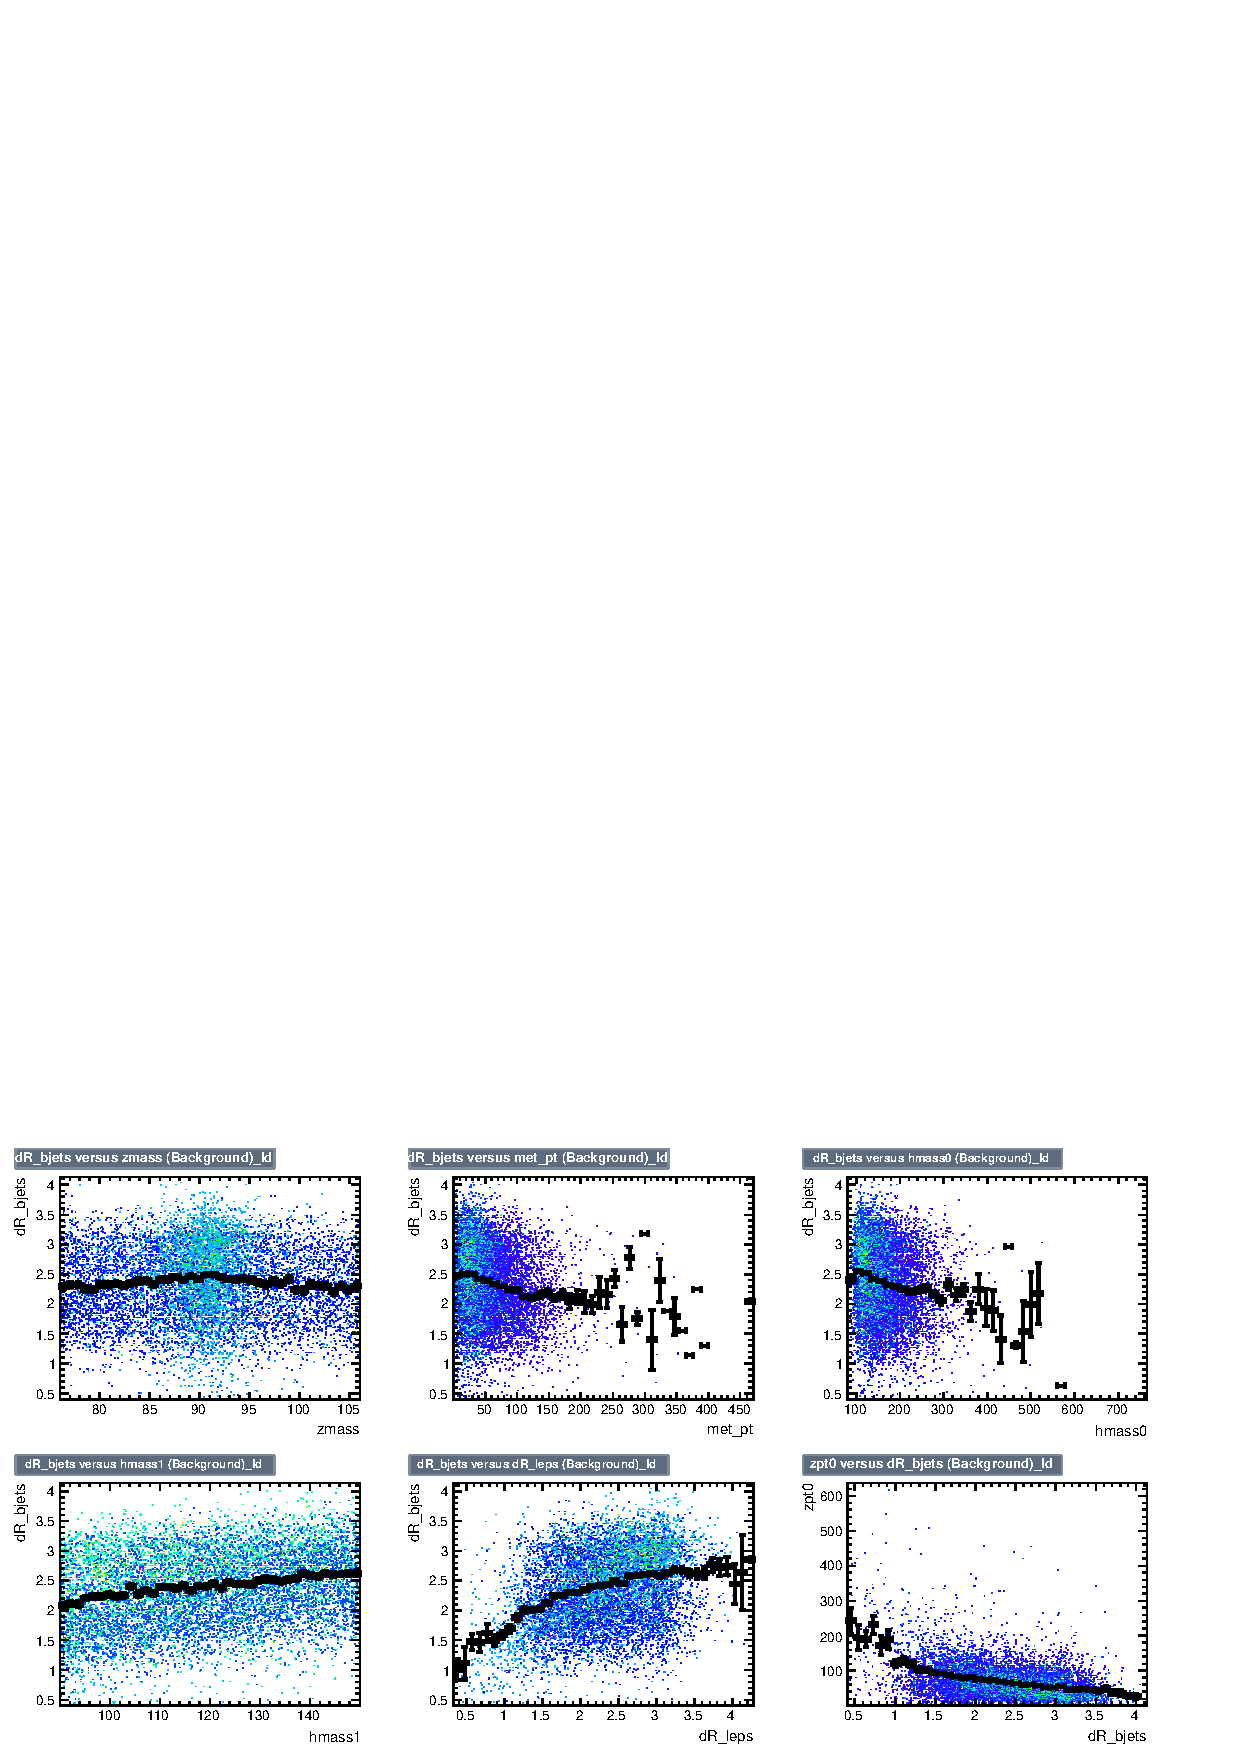
\includegraphics[width=0.95\textwidth]{figures/CRTT/dataset/plots/correlationscatter_dR_bjets__Id_c3.pdf}
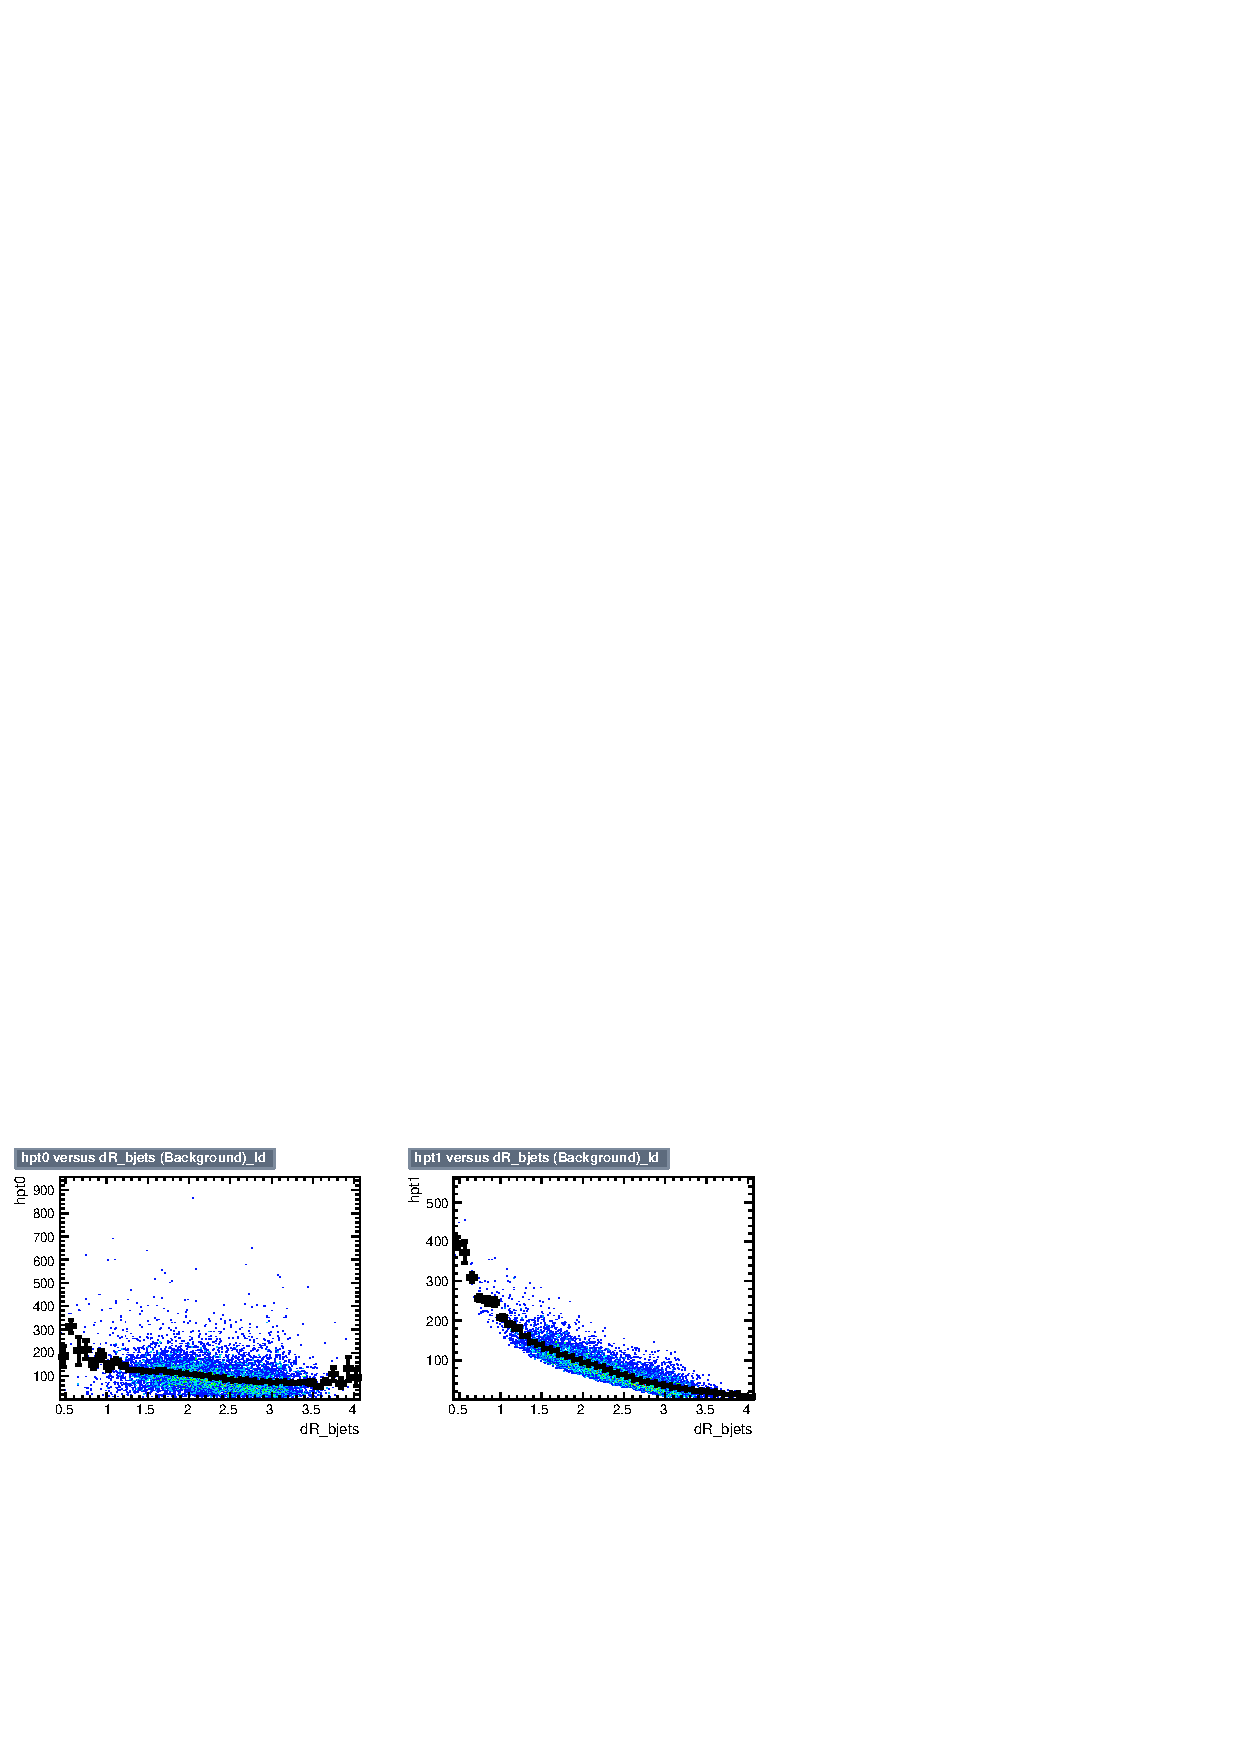
\includegraphics[width=0.95\textwidth]{figures/CRTT/dataset/plots/correlationscatter_dR_bjets__Id_c4.pdf}
\caption{ Correlation scatter plots for dR between bjets variable for backgrounds}%, index '1' refers to bb and index '0' refers to ZZ}
\label{fig:correlations_CRTT_drbjets_BG}                                                       
\end{figure}




\begin{figure}[!htb]%hbpt?        
\centering
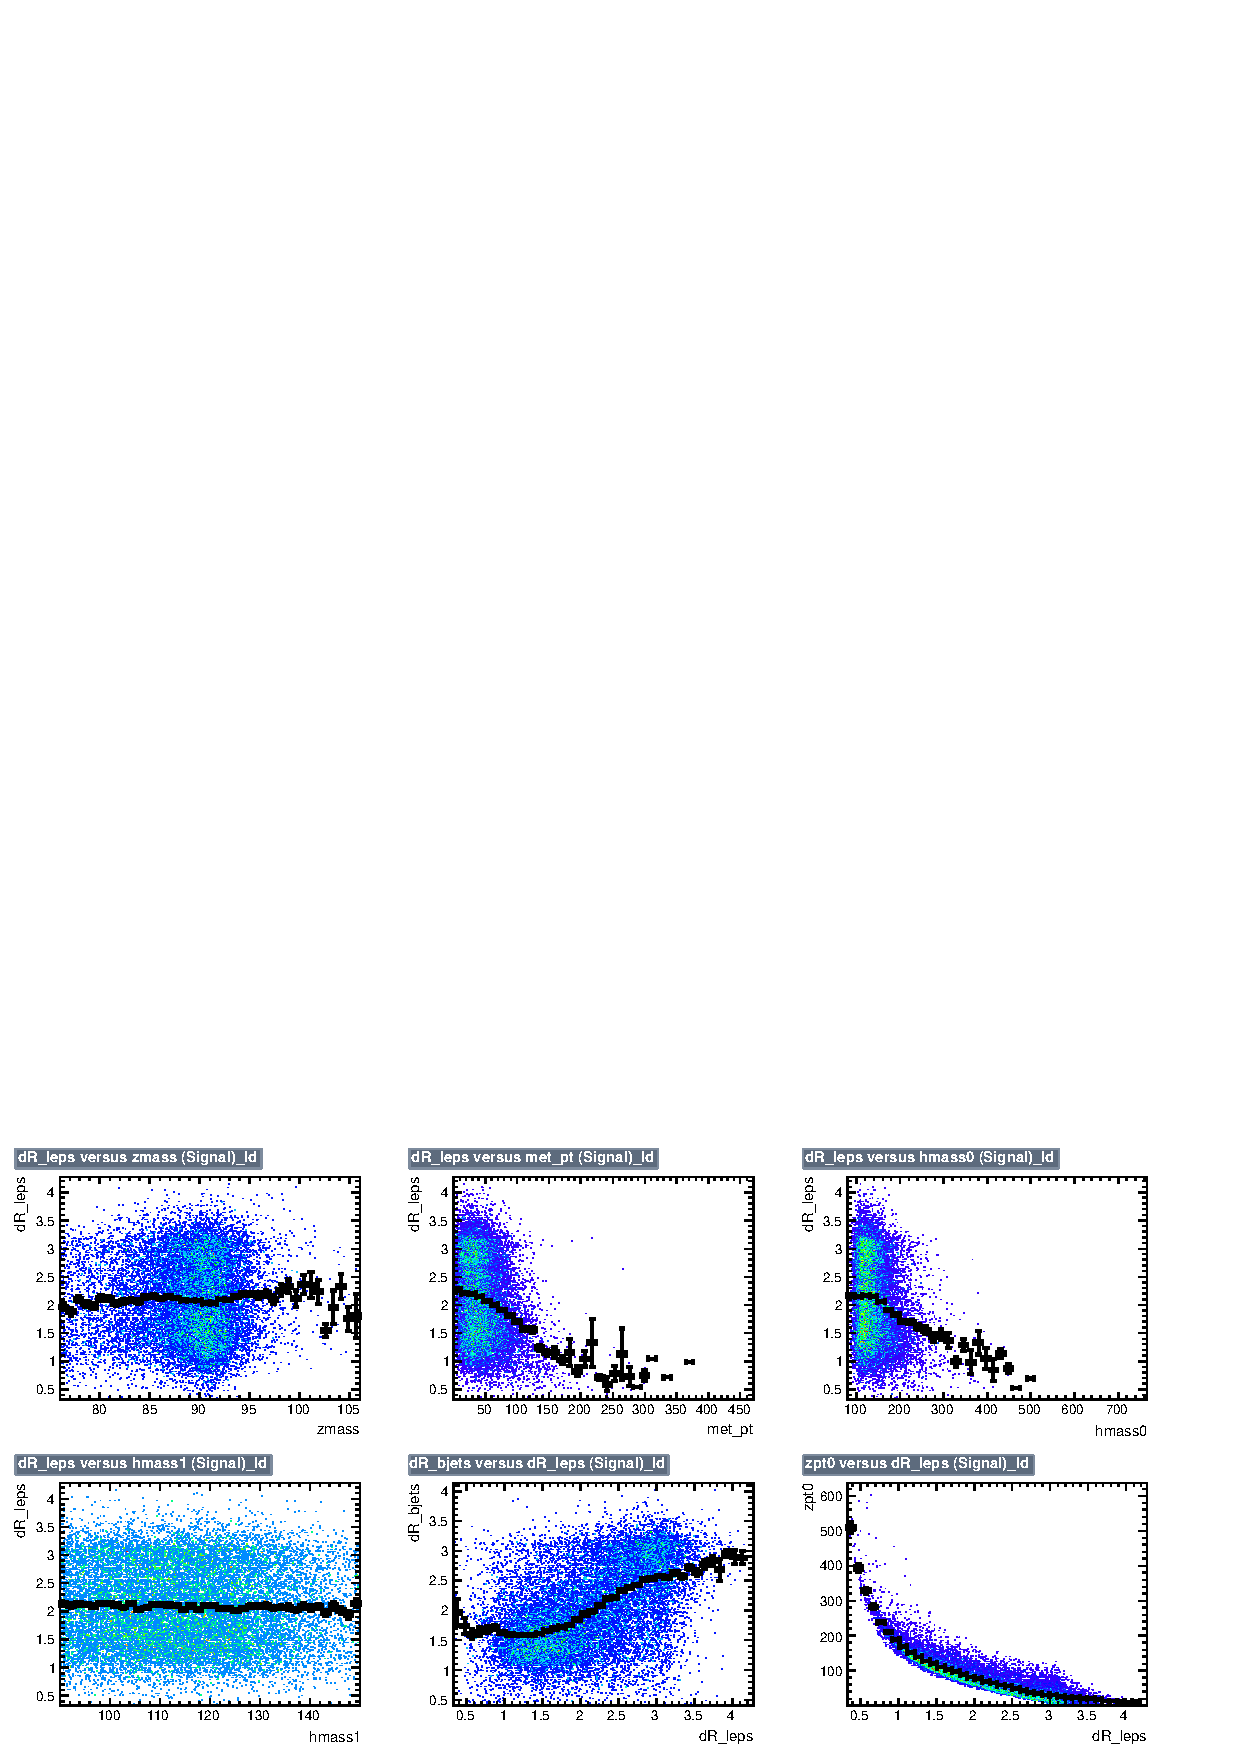
\includegraphics[width=0.95\textwidth]{figures/CRTT/dataset/plots/correlationscatter_dR_leps__Id_c1.pdf}
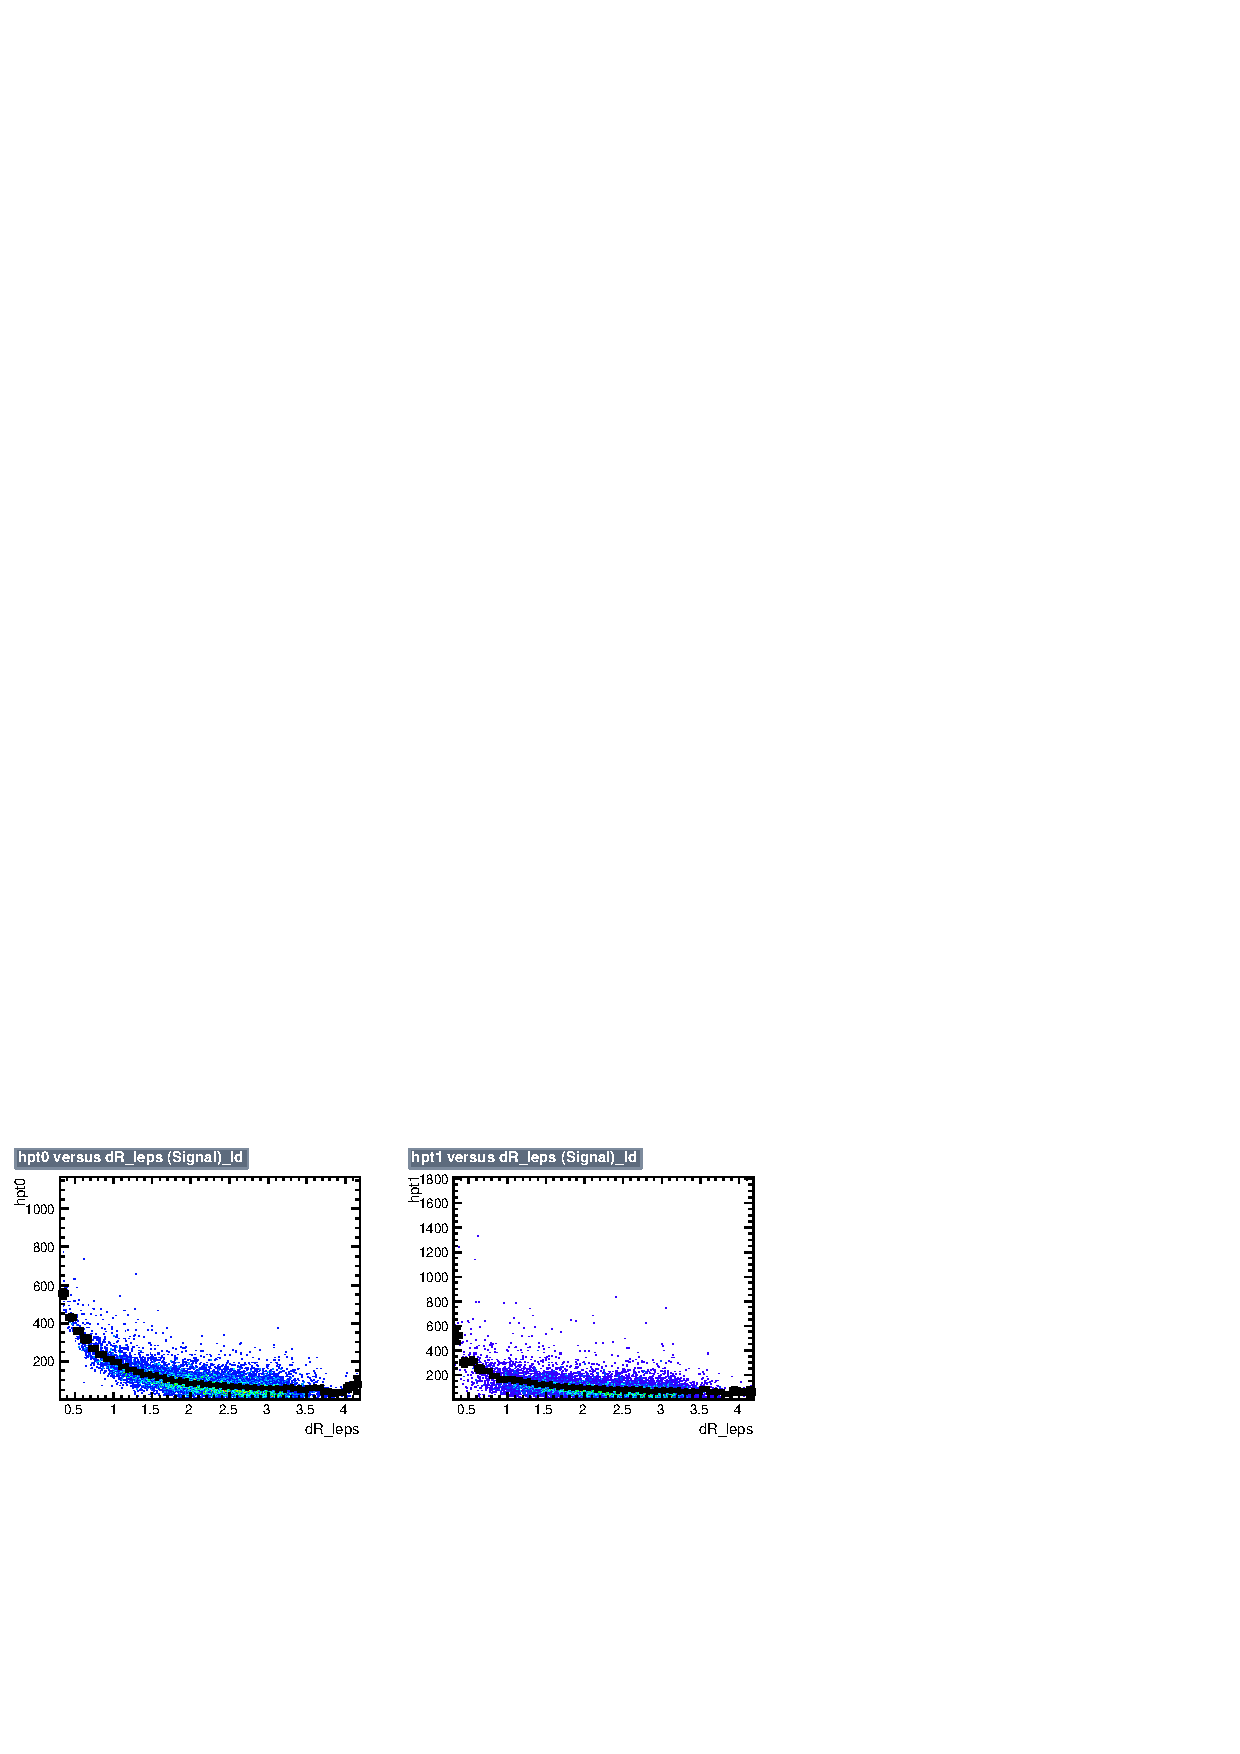
\includegraphics[width=0.95\textwidth]{figures/CRTT/dataset/plots/correlationscatter_dR_leps__Id_c2.pdf}
\caption{ Correlation scatter plots for dR between leptons variable for data}%, index '1' refers to bb and index '0' refers to ZZ}
\label{fig:correlations_CRTT_drleps_S}                                                       
\end{figure}



\begin{figure}[!htb]%hbpt?        
\centering
\includegraphics[width=0.95\textwidth]{figures/CRTT/dataset/plots/correlationscatter_dR_leps__Id_c3.pdf}
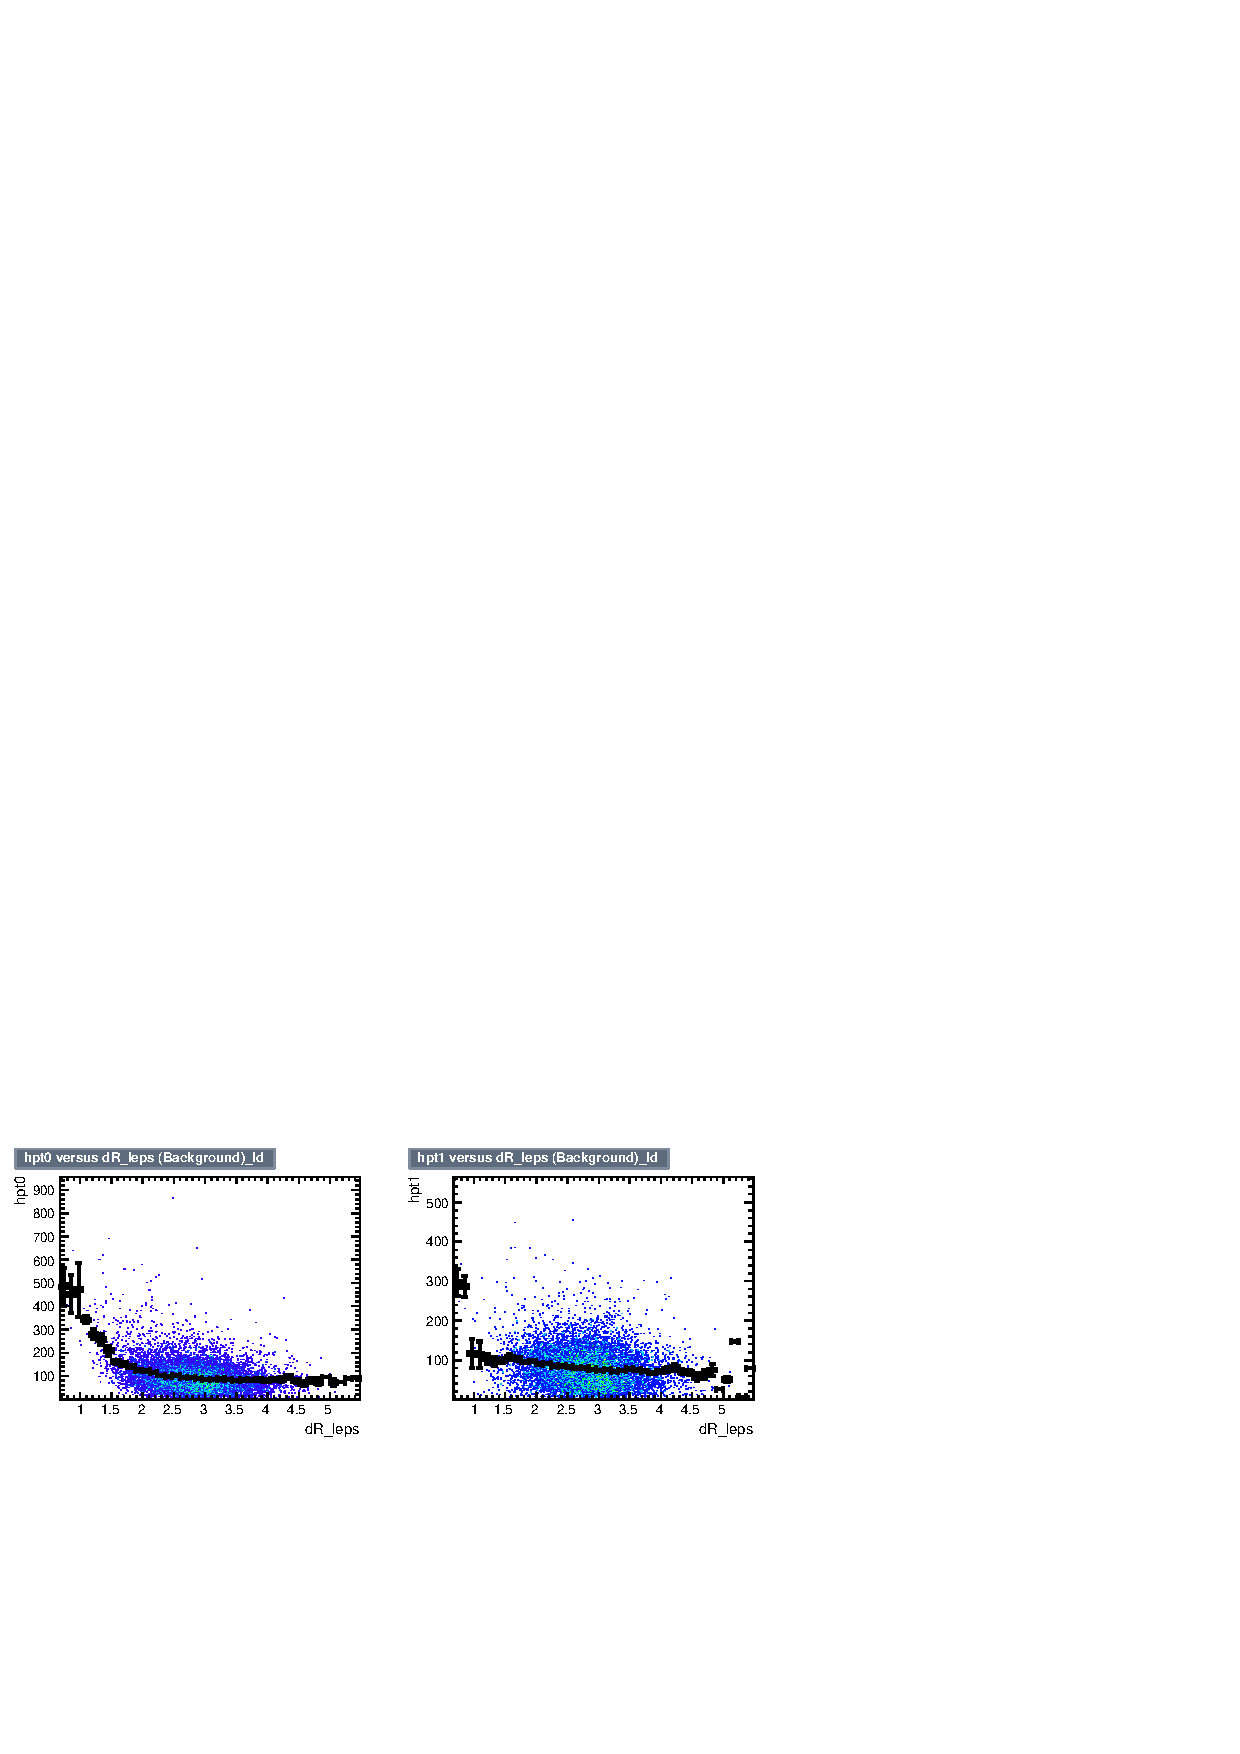
\includegraphics[width=0.95\textwidth]{figures/CRTT/dataset/plots/correlationscatter_dR_leps__Id_c4.pdf}
\caption{ Correlation scatter plots for dR between keptons variable for backgrounds}%, index '1' refers to bb and index '0' refers to ZZ}
\label{fig:correlations_CRTT_drleps_BG}                                                       
\end{figure}



\begin{figure}[!htb]%hbpt?        
\centering
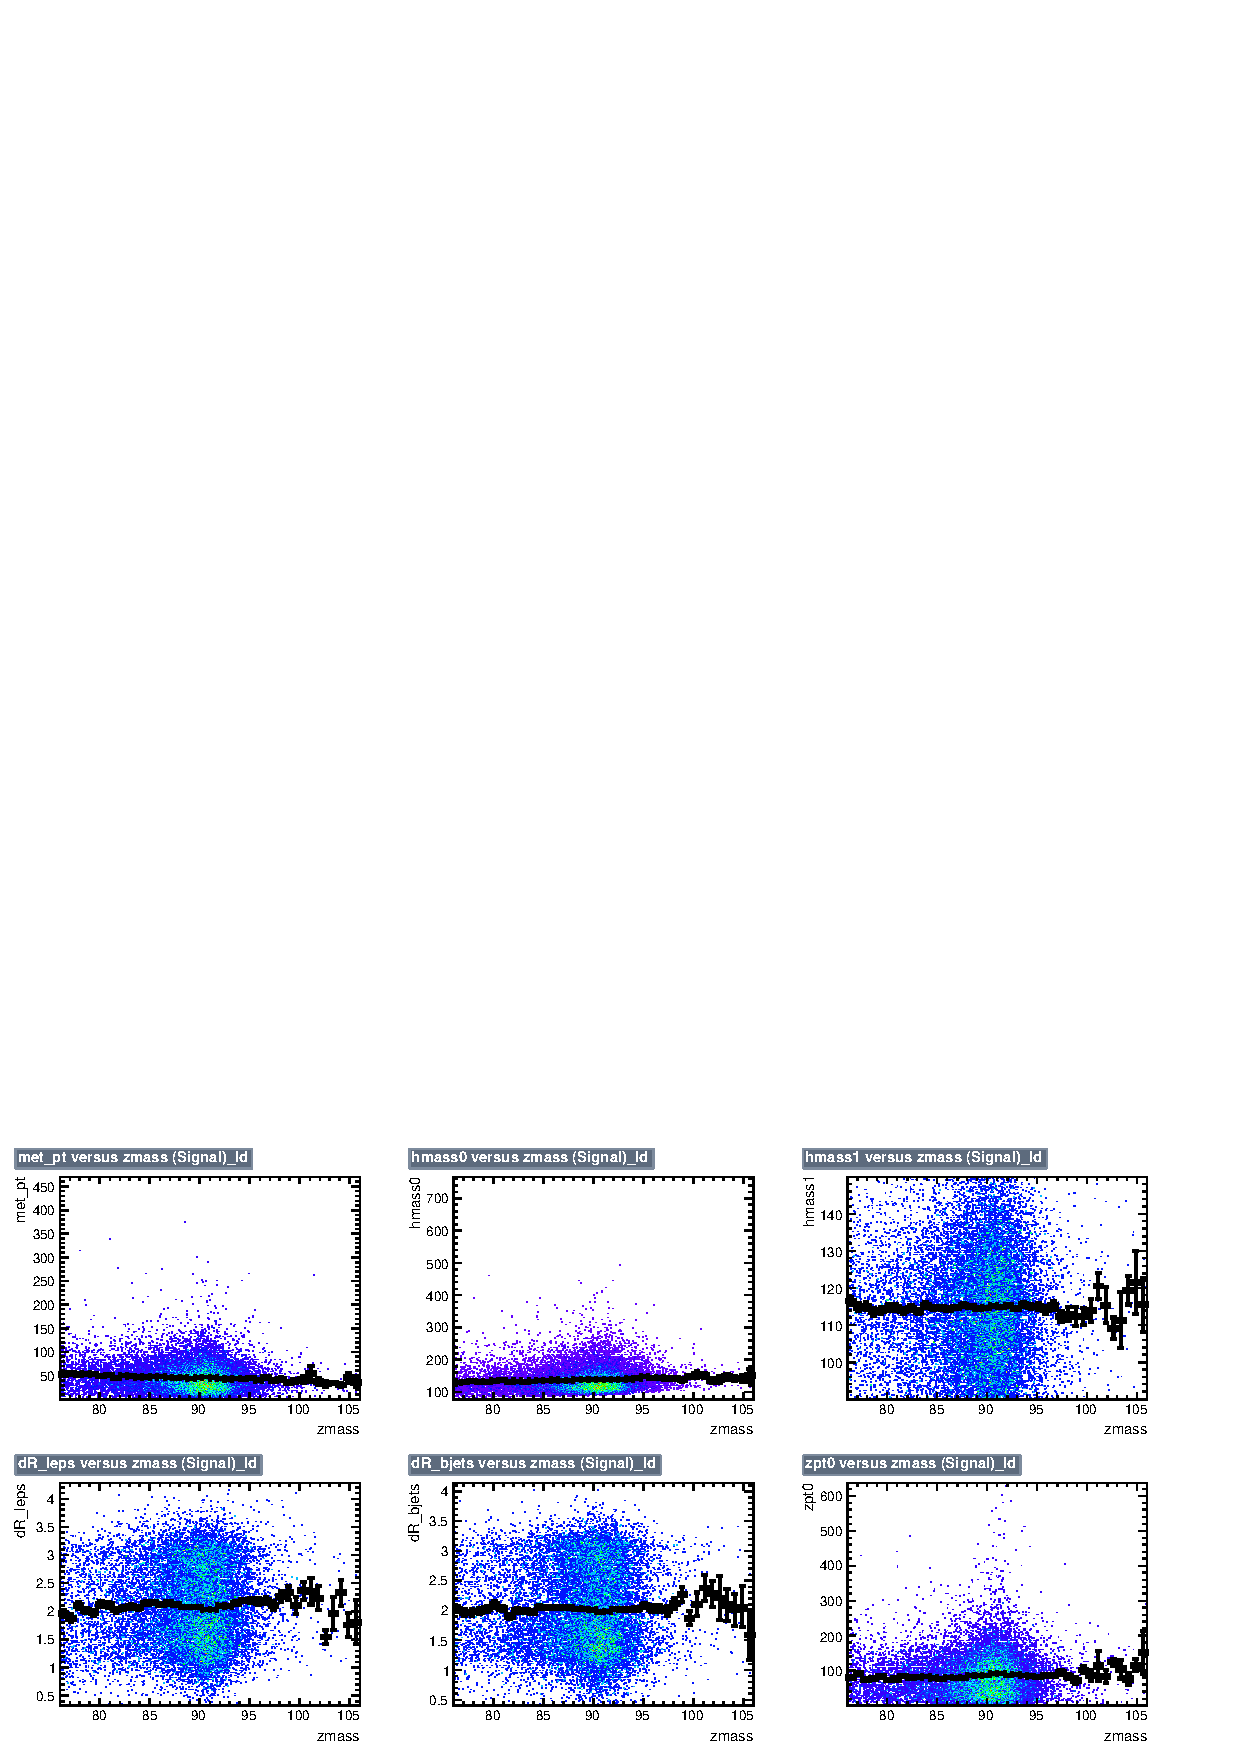
\includegraphics[width=0.95\textwidth]{figures/CRTT/dataset/plots/correlationscatter_zmass__Id_c1.pdf}
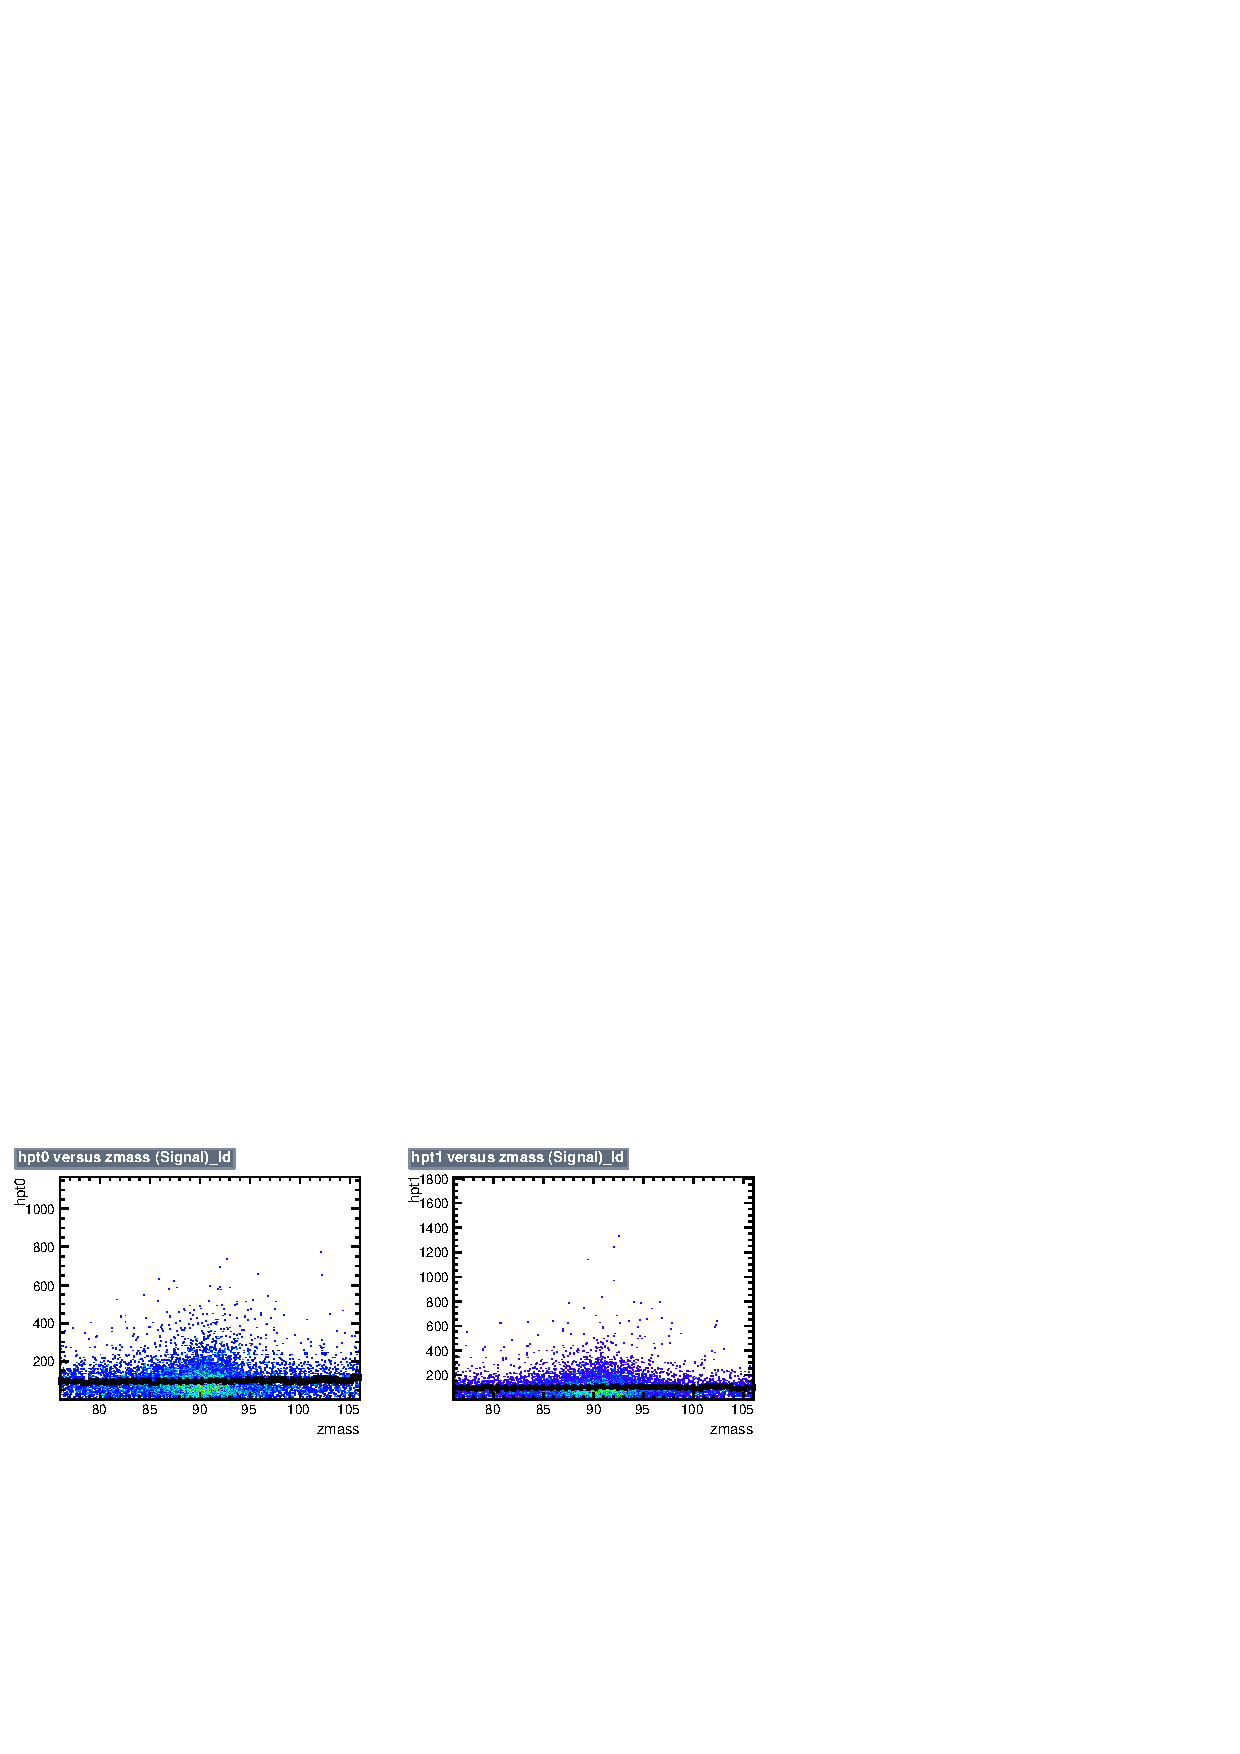
\includegraphics[width=0.95\textwidth]{figures/CRTT/dataset/plots/correlationscatter_zmass__Id_c2.pdf}
\caption{ Correlation scatter plots for \Zll bjets variable for data}%, index '1' refers to bb and index '0' refers to ZZ}
\label{fig:correlations_CRTT_zmass_S}                                                       
\end{figure}



\begin{figure}[!htb]%hbpt?        
\centering
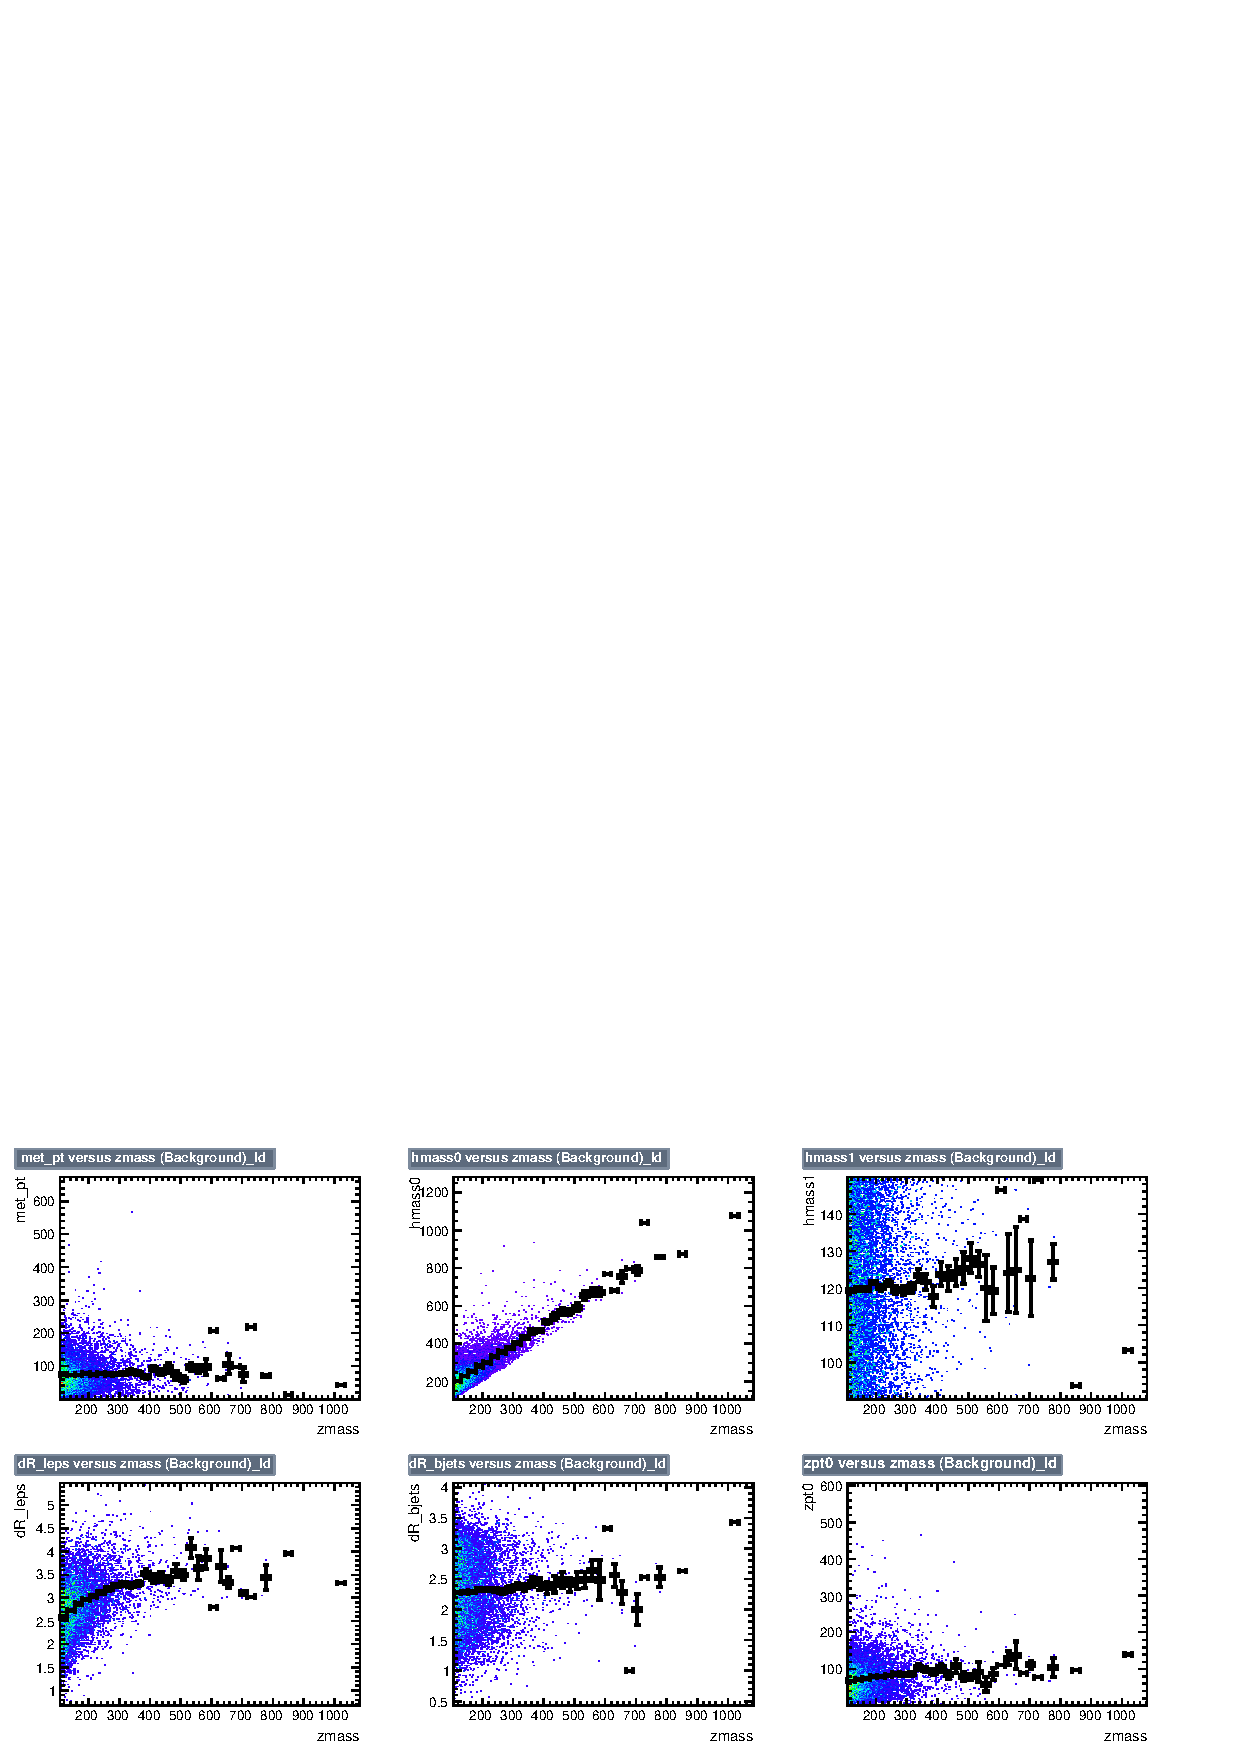
\includegraphics[width=0.95\textwidth]{figures/CRTT/dataset/plots/correlationscatter_zmass__Id_c3.pdf}
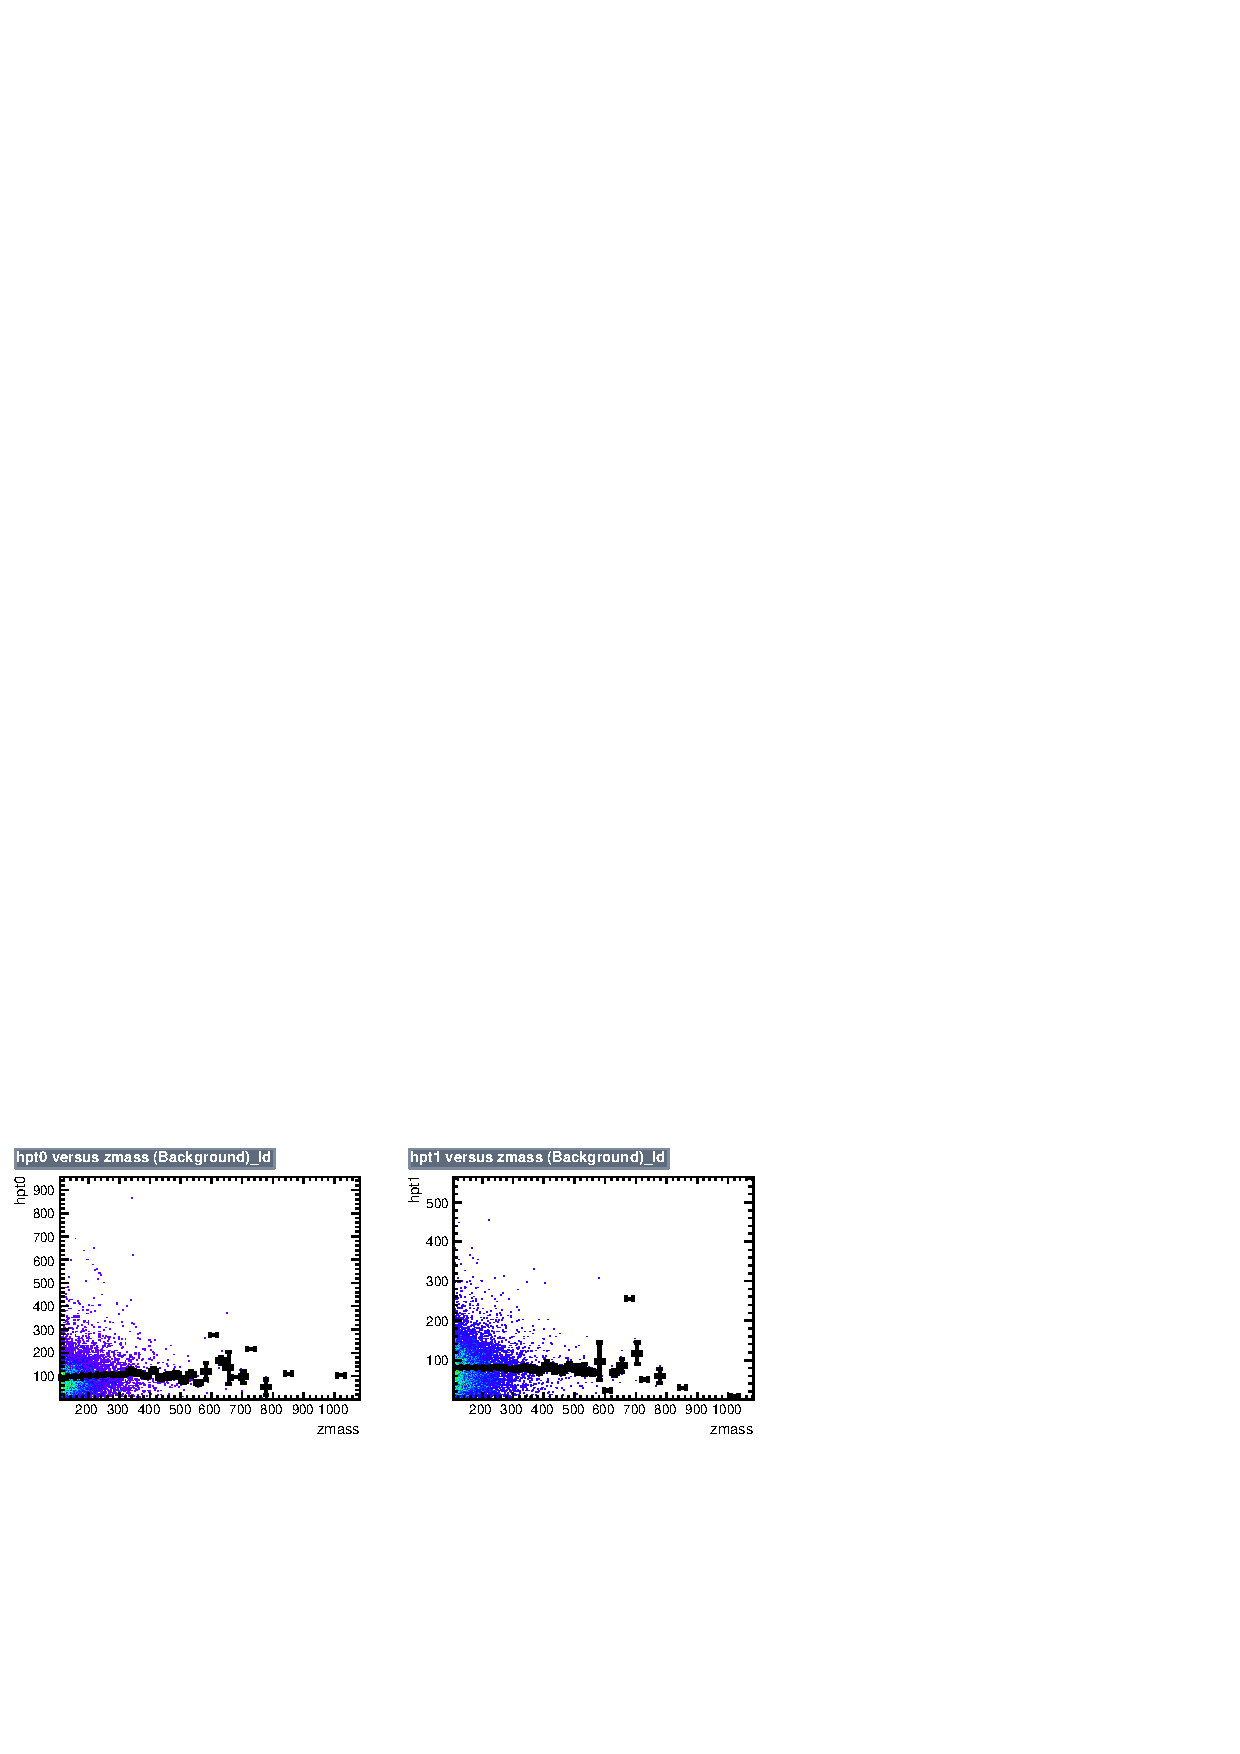
\includegraphics[width=0.95\textwidth]{figures/CRTT/dataset/plots/correlationscatter_zmass__Id_c4.pdf}
\caption{ Correlation scatter plots for \Zll mass variable for backgrounds}%, index '1' refers to bb and index '0' refers to ZZ}
\label{fig:correlations_CRTT_zmass_BG}                                                       
\end{figure}



\begin{figure}[!htb]%hbpt?        
\centering
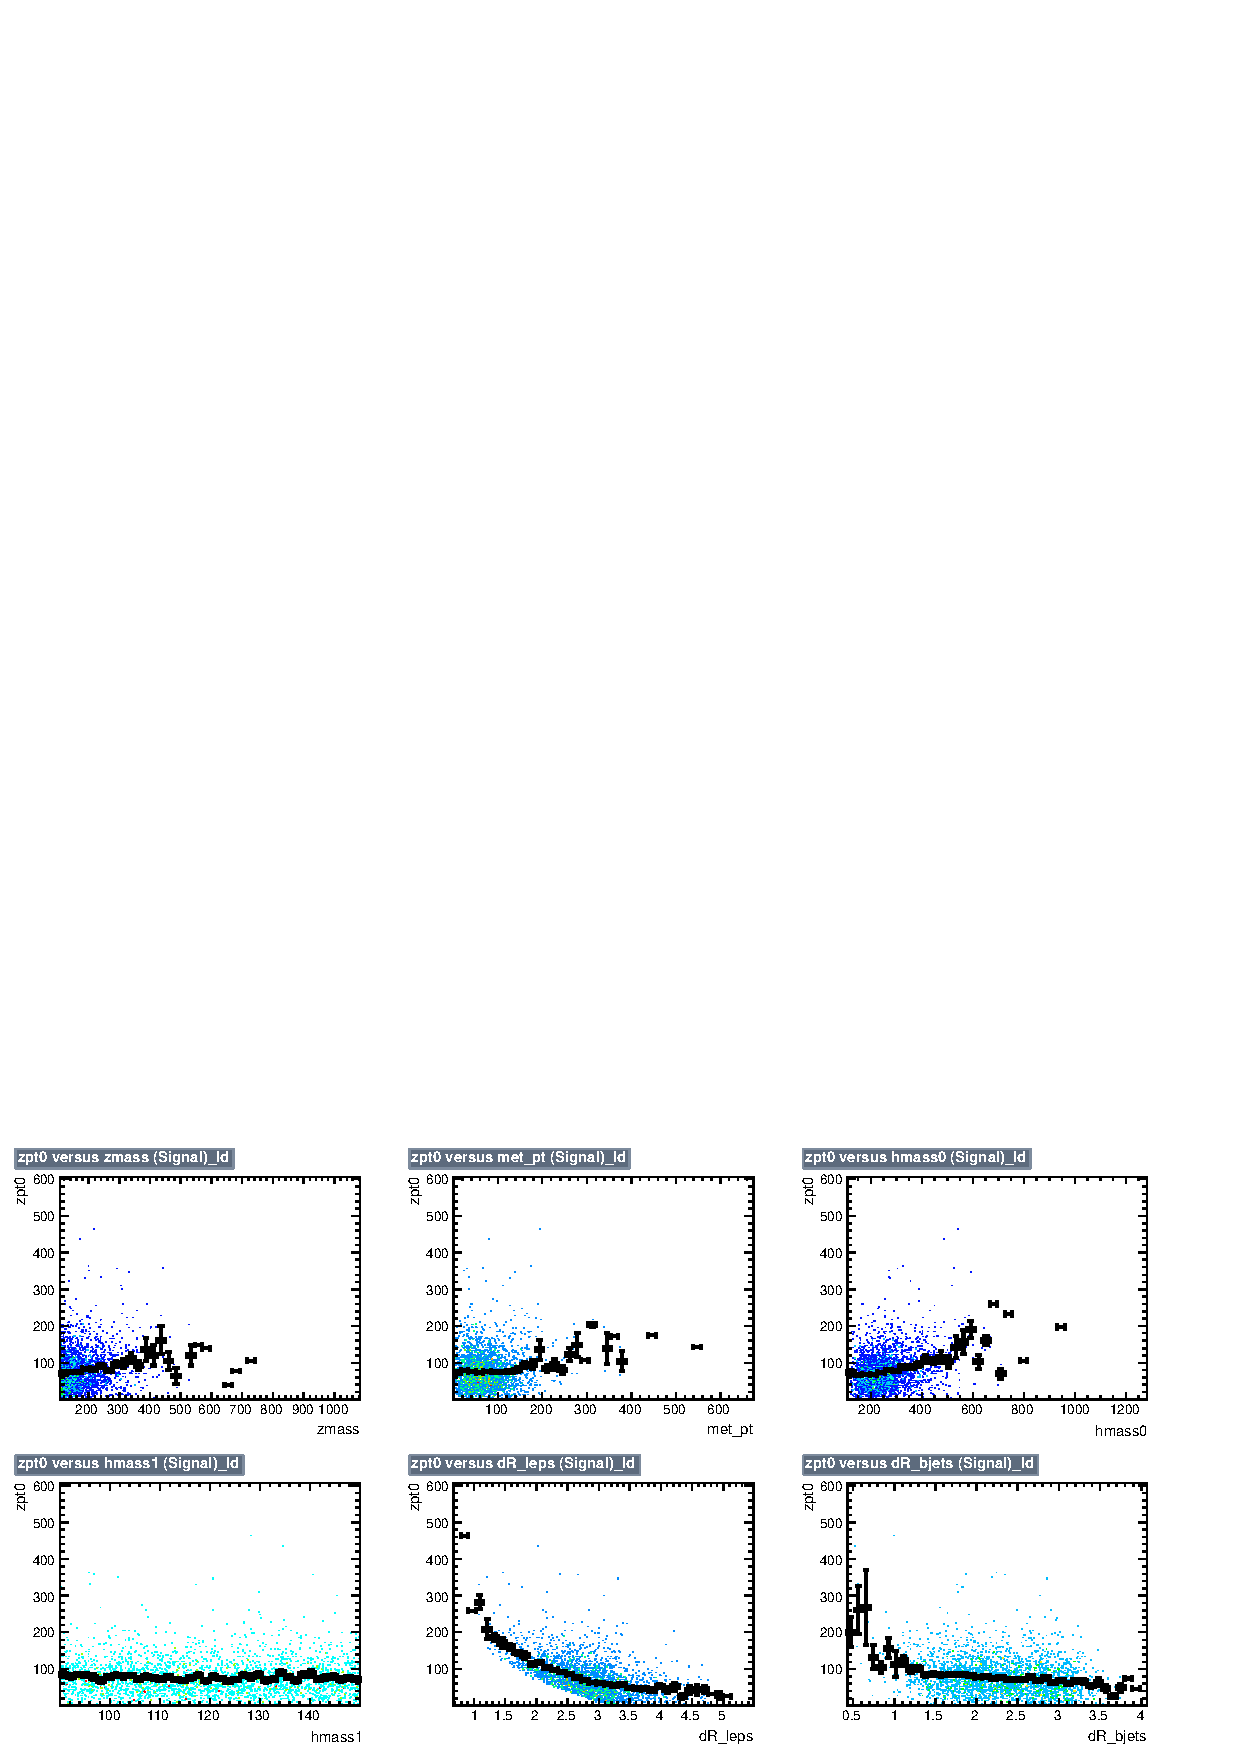
\includegraphics[width=0.95\textwidth]{figures/CRTT/dataset/plots/correlationscatter_zpt0__Id_c1.pdf}
\includegraphics[width=0.95\textwidth]{figures/CRTT/dataset/plots/correlationscatter_zpt0__Id_c2.pdf}
\caption{ Correlation scatter plots for Z $p_{T}$  variable for data}%, index '1' refers to bb and index '0' refers to ZZ}
\label{fig:correlations_CRTT_zpt_S}                                                       
\end{figure}



\begin{figure}[!htb]%hbpt?        
\centering
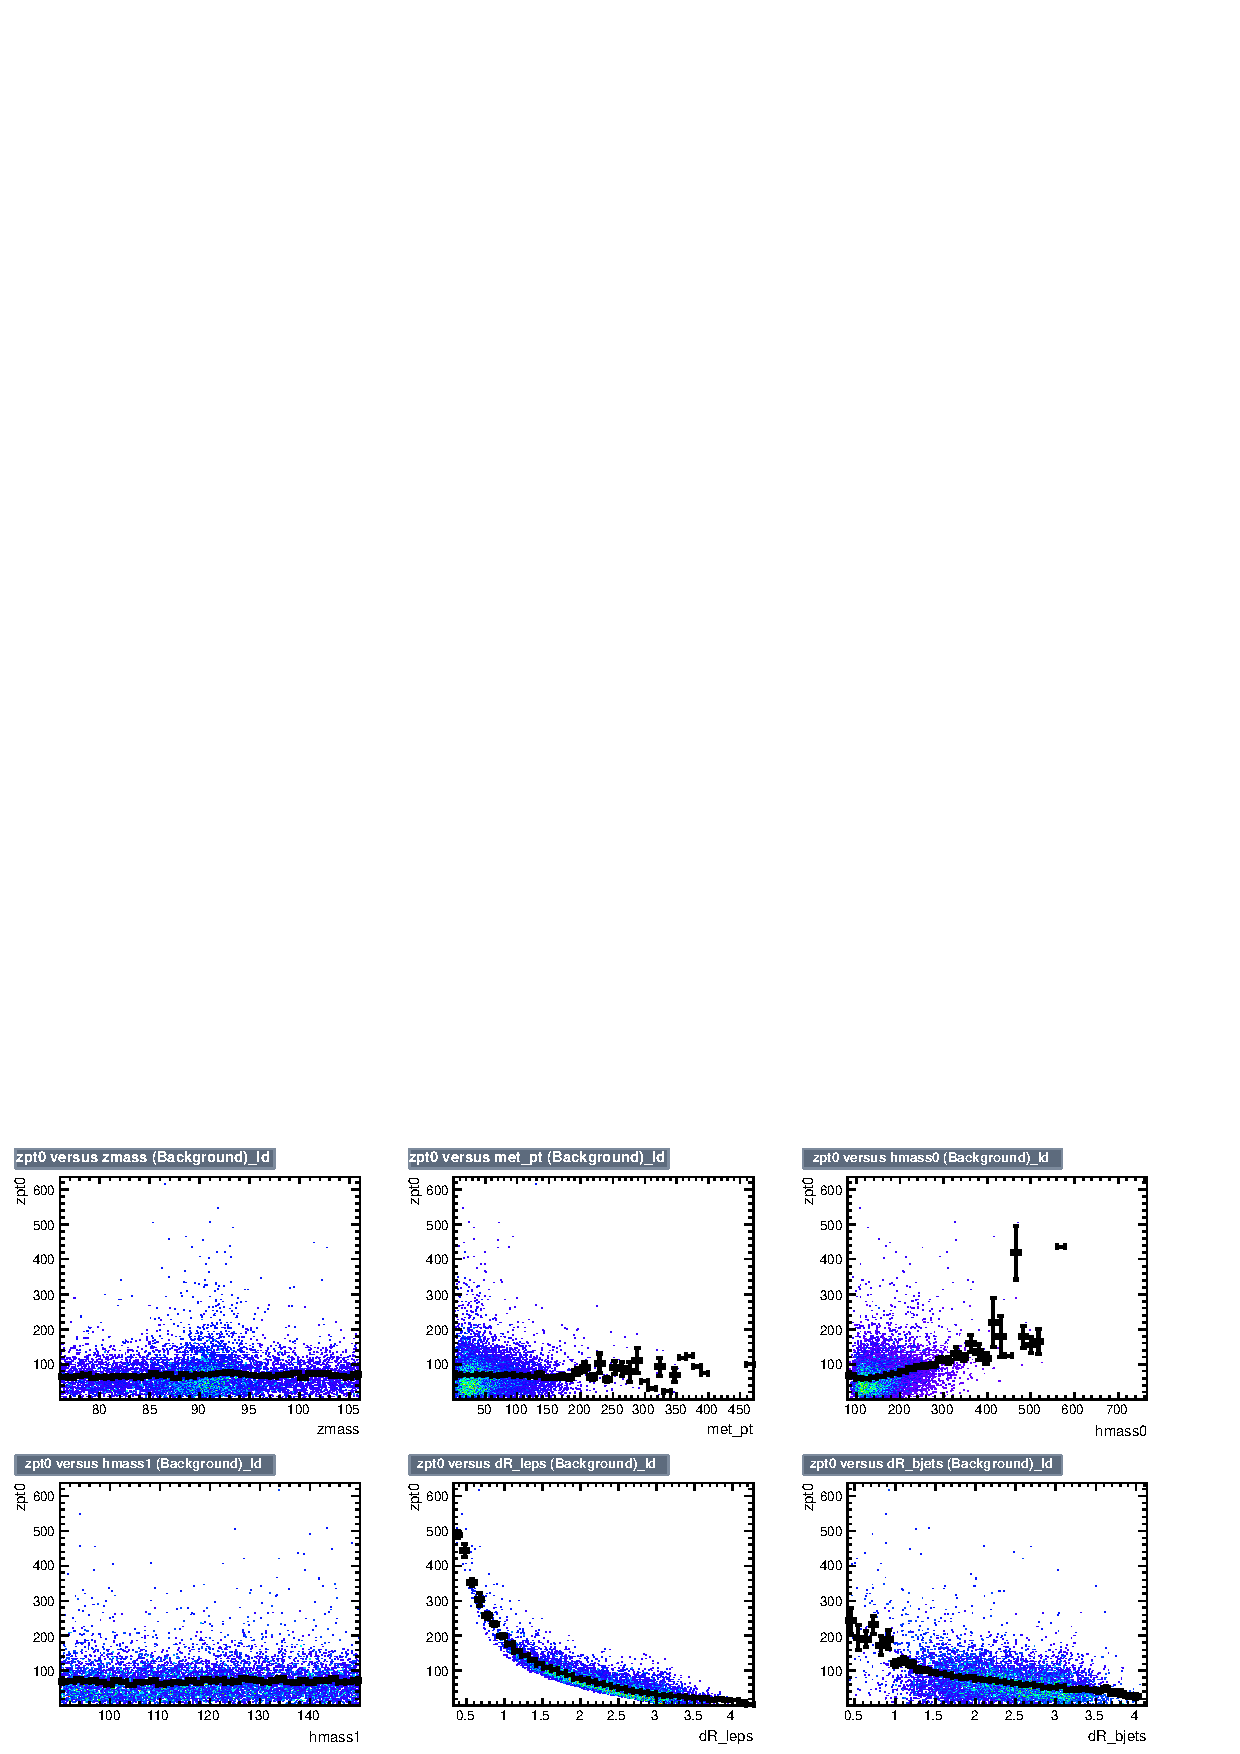
\includegraphics[width=0.95\textwidth]{figures/CRTT/dataset/plots/correlationscatter_zpt0__Id_c3.pdf}
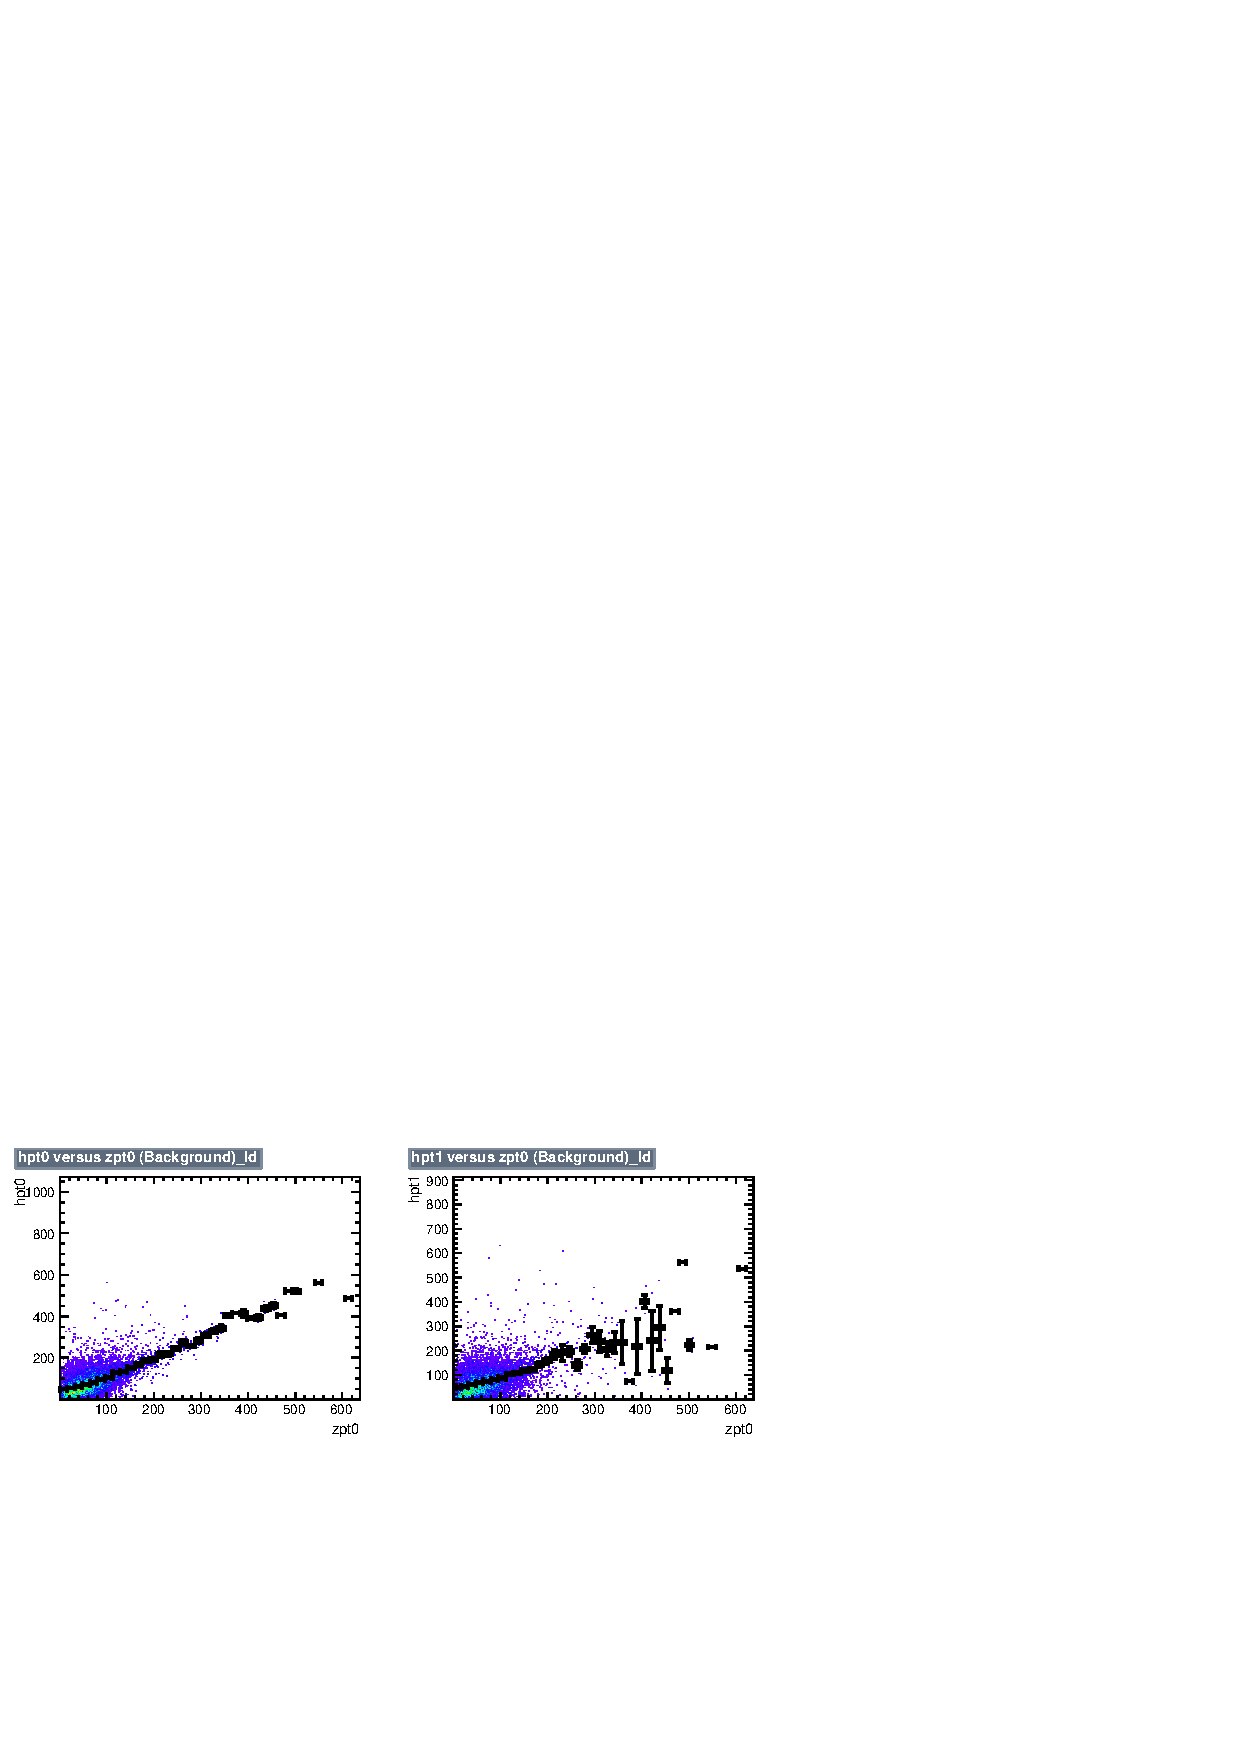
\includegraphics[width=0.95\textwidth]{figures/CRTT/dataset/plots/correlationscatter_zpt0__Id_c4.pdf}
\caption{ Correlation scatter plots for Z $p_{T}$ variable for backgrounds}%, index '1' refers to bb and index '0' refers to ZZ}
\label{fig:correlations_CRTT_zpt_BG}                                                       
\end{figure}


\begin{figure}[!htb]%hbpt?        
\centering
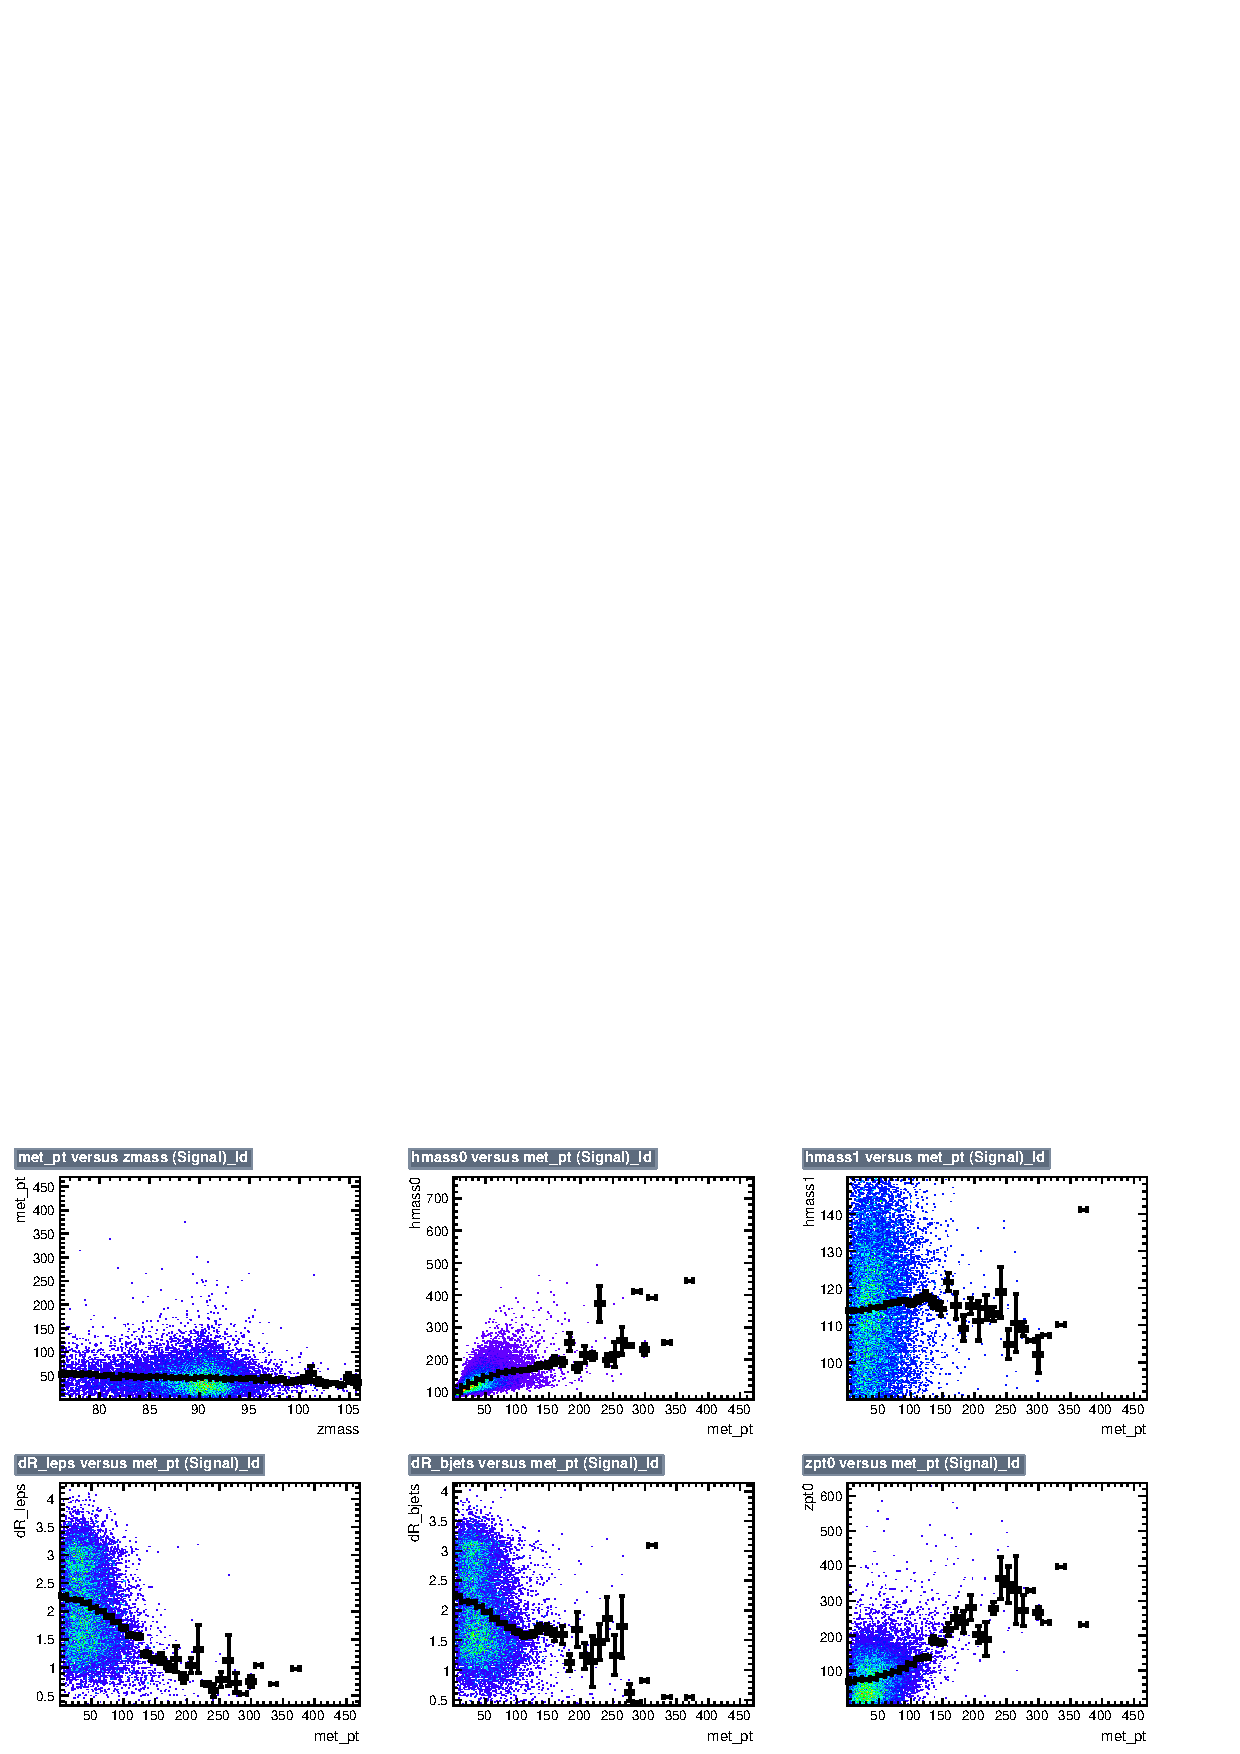
\includegraphics[width=0.95\textwidth]{figures/CRTT/dataset/plots/correlationscatter_met_pt__Id_c1.pdf}
\includegraphics[width=0.95\textwidth]{figures/CRTT/dataset/plots/correlationscatter_met_pt__Id_c2.pdf}
\caption{ Correlation scatter plots for met variable for data}%, index '1' refers to bb and index '0' refers to ZZ}
\label{fig:correlations_CRTT_met_pt_S}                                                       
\end{figure}



\begin{figure}[!htb]%hbpt?        
\centering
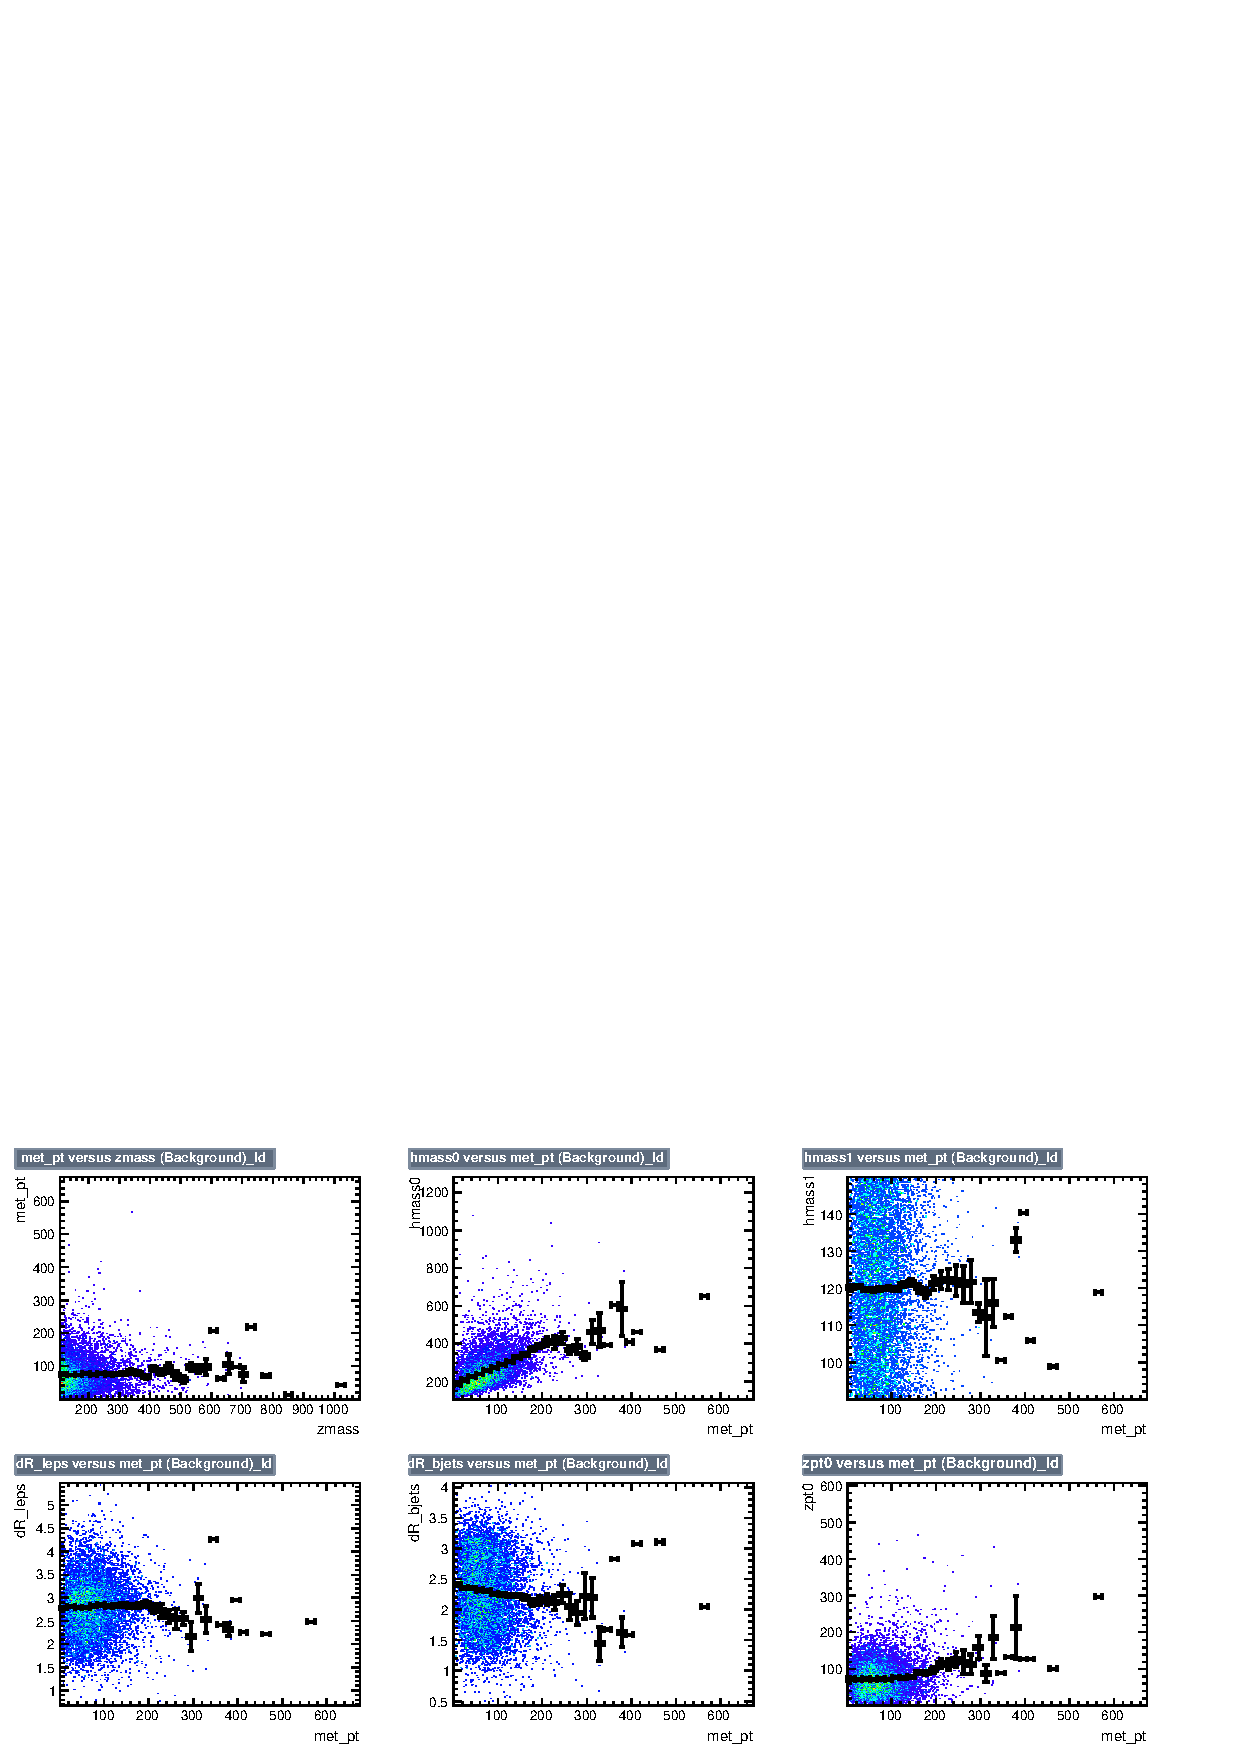
\includegraphics[width=0.95\textwidth]{figures/CRTT/dataset/plots/correlationscatter_met_pt__Id_c3.pdf}
\includegraphics[width=0.95\textwidth]{figures/CRTT/dataset/plots/correlationscatter_met_pt__Id_c4.pdf}
\caption{ Correlation scatter plots for met variable for backgrounds}%, index '1' refers to bb and index '0' refers to ZZ}
\label{fig:correlations_CRTT_met_pt_BG}                                                       
\end{figure}





\begin{figure}[!htb]%hbpt?        
\centering
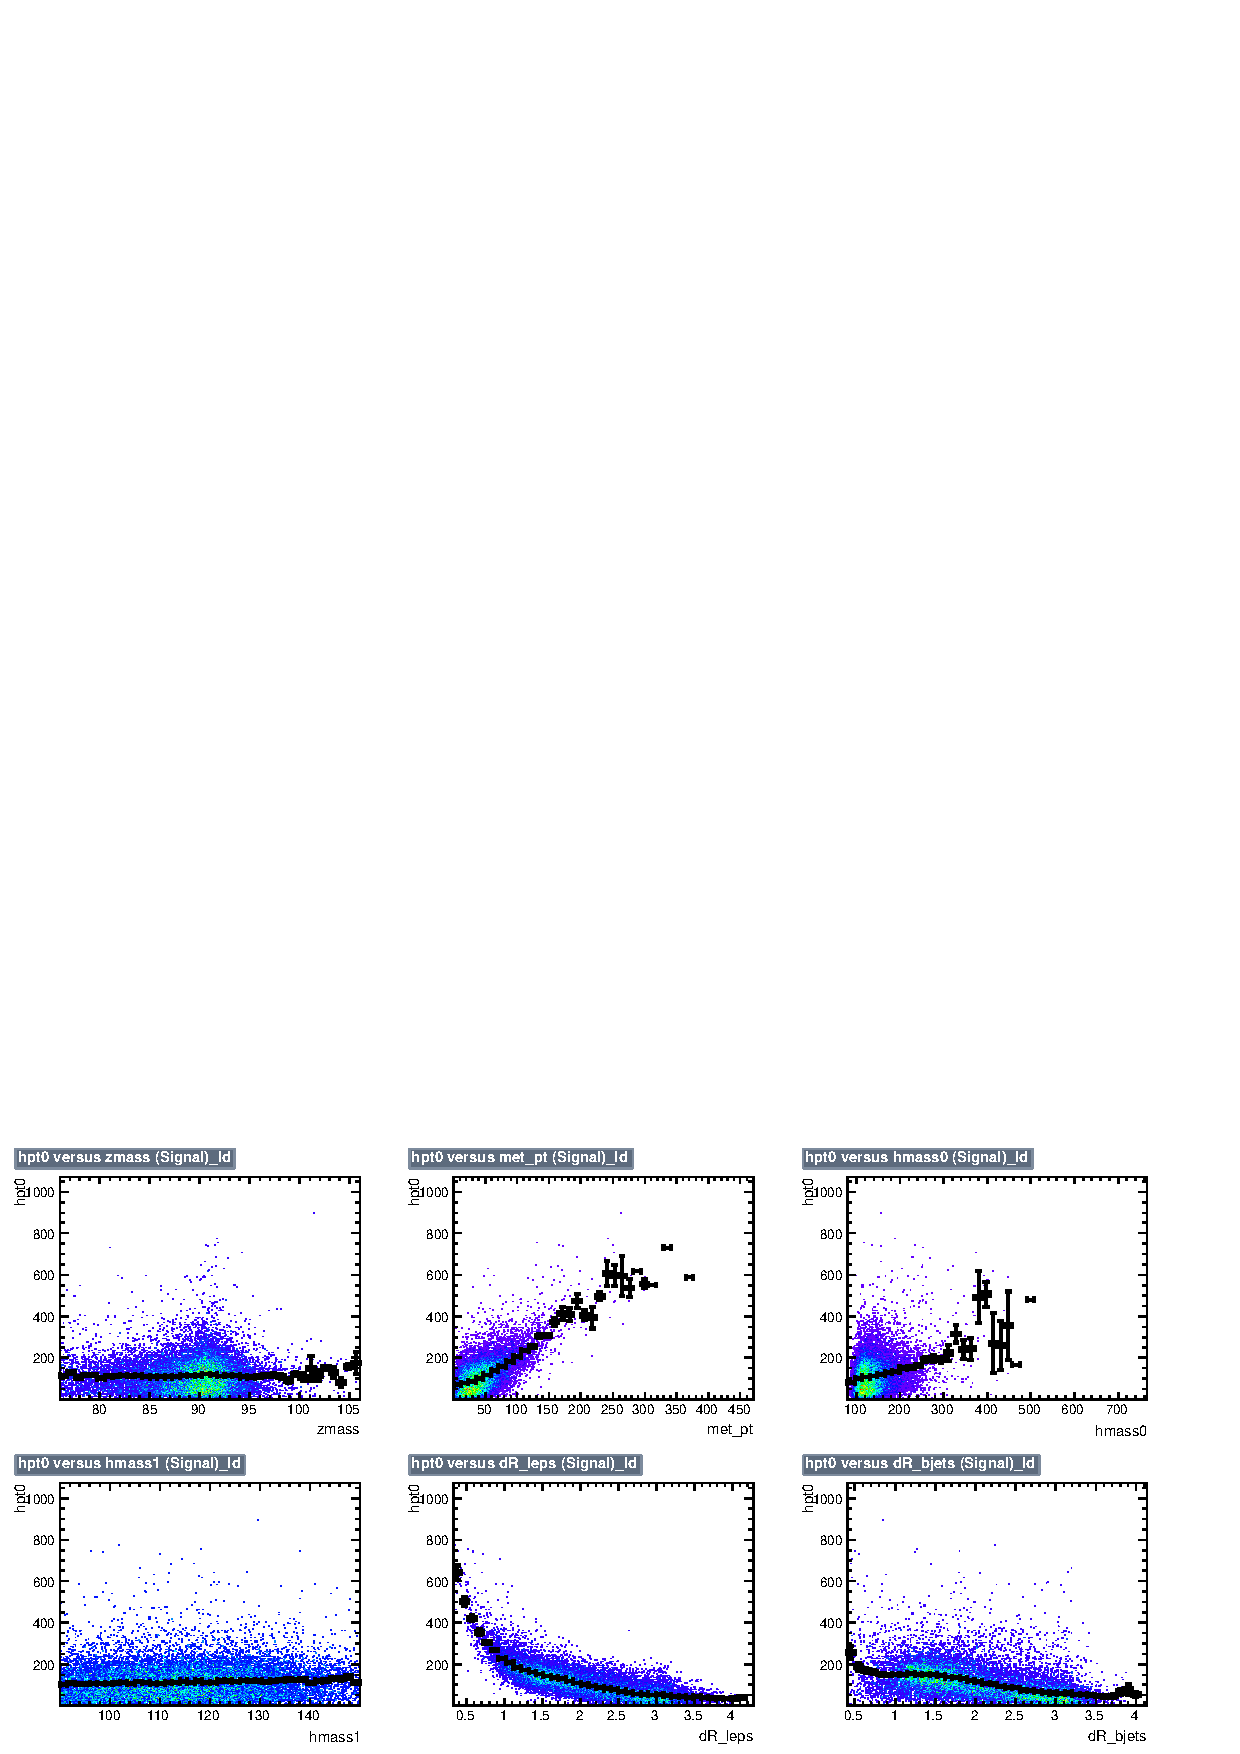
\includegraphics[width=0.95\textwidth]{figures/CRTT/dataset/plots/correlationscatter_hpt0__Id_c1.pdf}
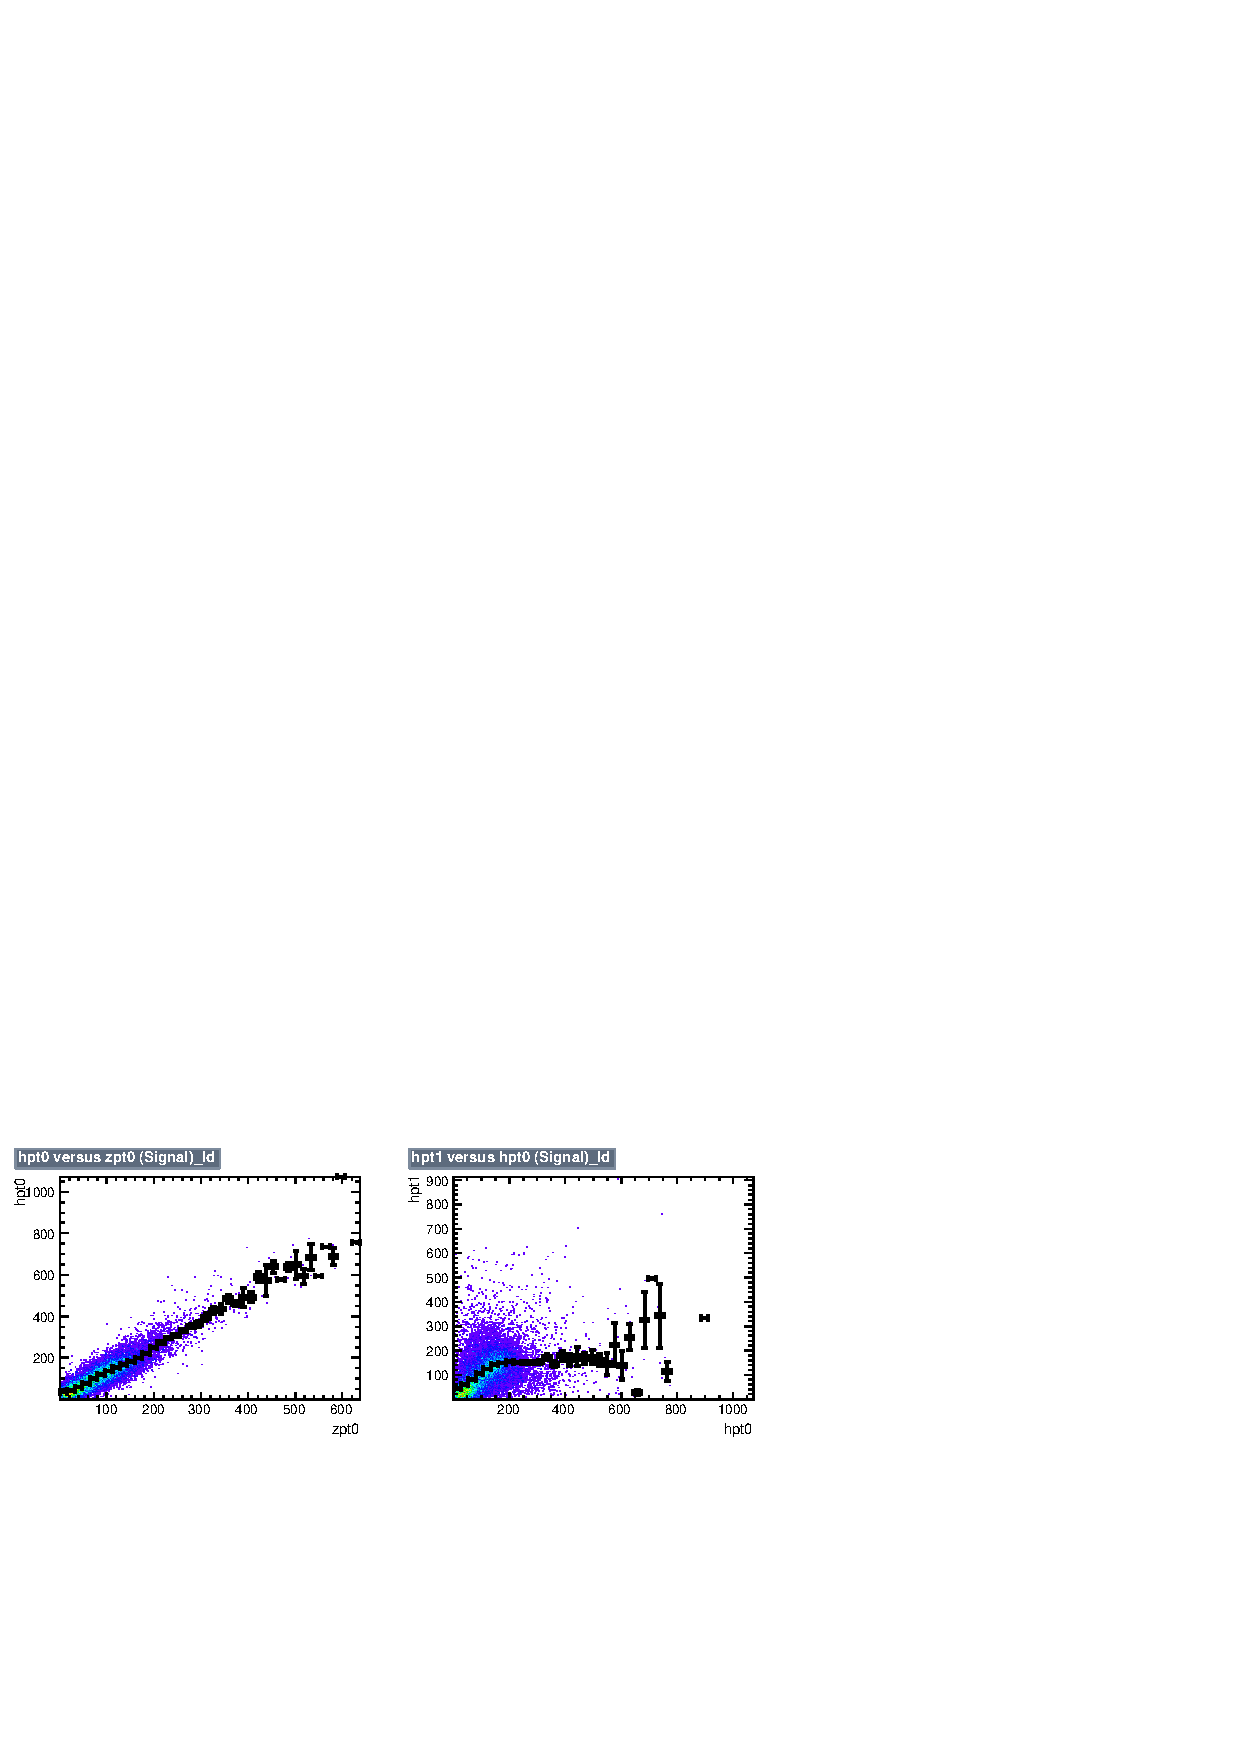
\includegraphics[width=0.95\textwidth]{figures/CRTT/dataset/plots/correlationscatter_hpt0__Id_c2.pdf}
\caption{ Correlation scatter plots for \HZZ $p_{T}$  variable for data}%, index '1' refers to bb and index '0' refers to ZZ}
\label{fig:correlations_CRTT_hpt0_S}                                                       
\end{figure}



\begin{figure}[!htb]%hbpt?        
\centering
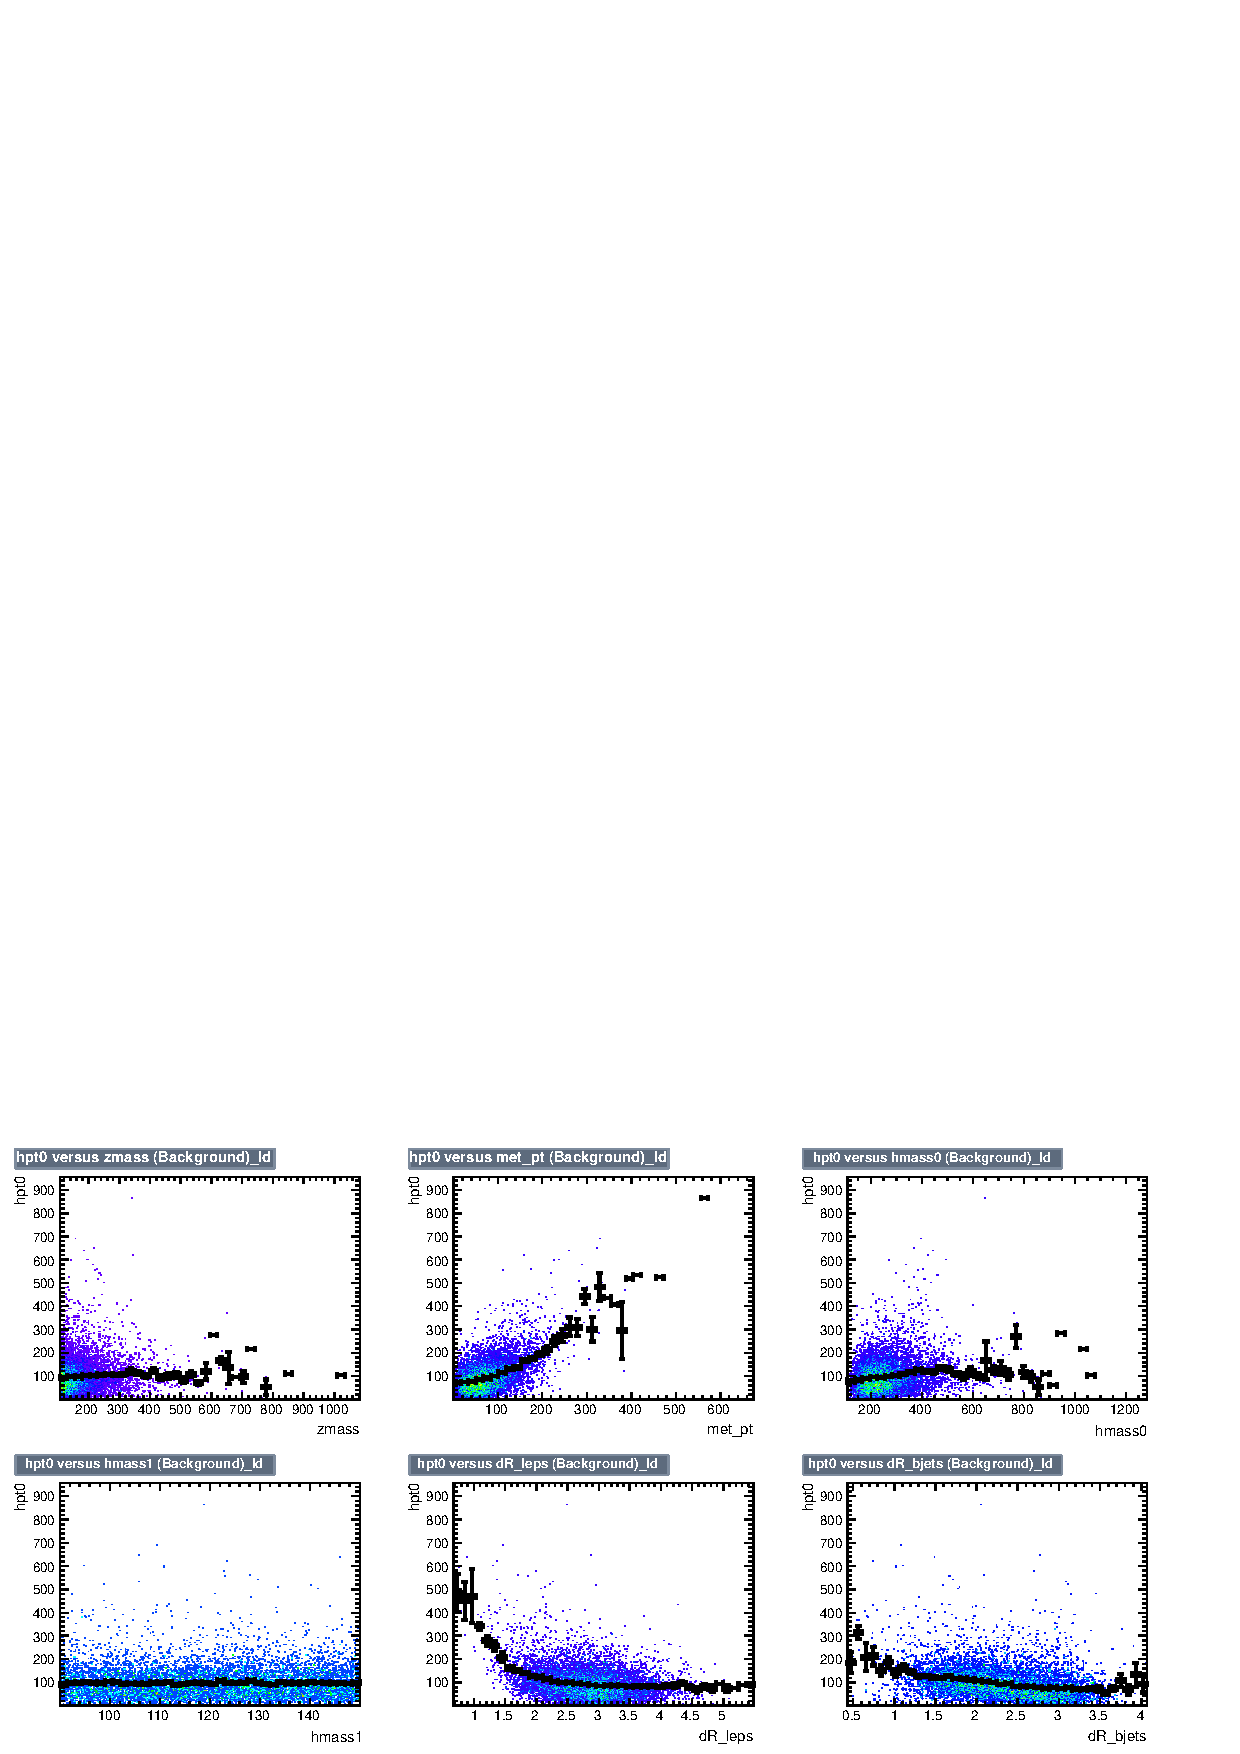
\includegraphics[width=0.95\textwidth]{figures/CRTT/dataset/plots/correlationscatter_hpt0__Id_c3.pdf}
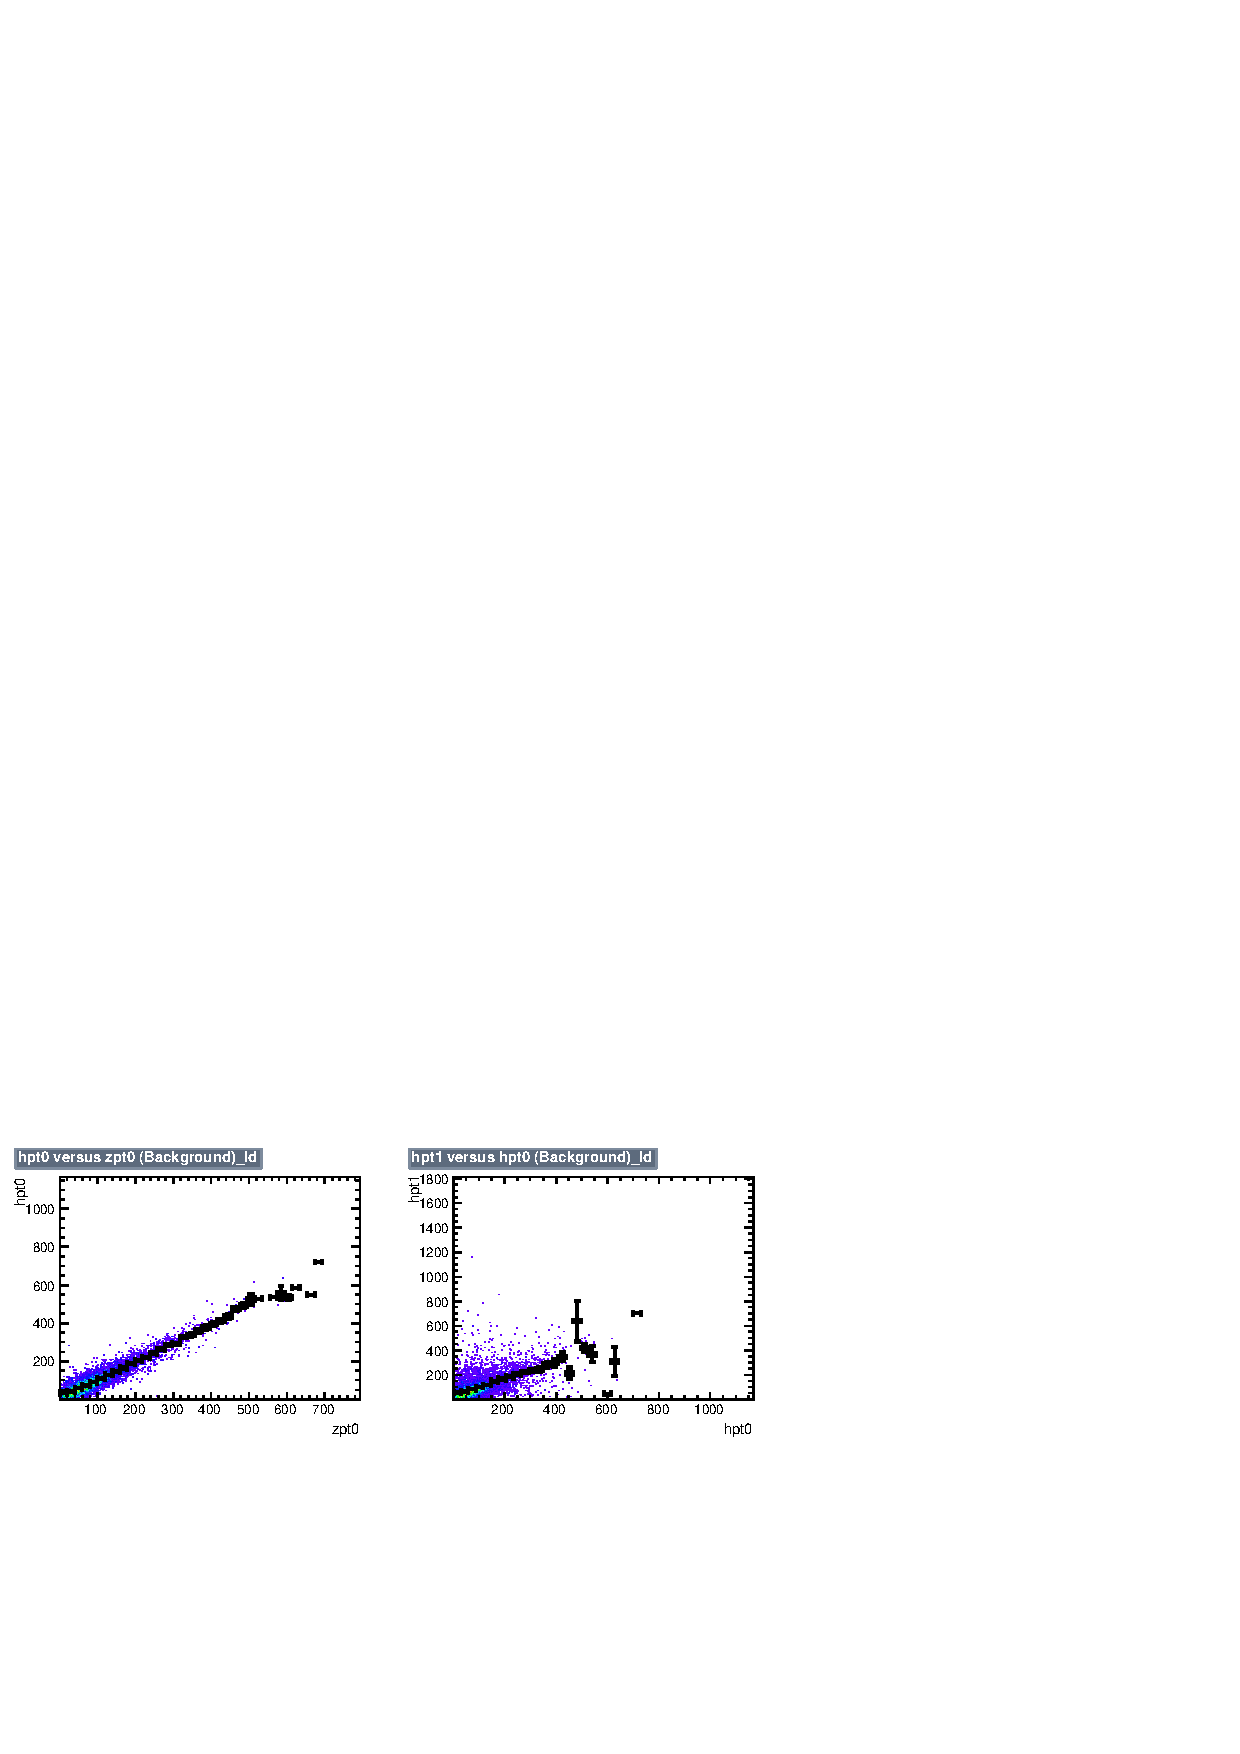
\includegraphics[width=0.95\textwidth]{figures/CRTT/dataset/plots/correlationscatter_hpt0__Id_c4.pdf}
\caption{ Correlation scatter plots for \HZZ $p_{T}$ variable for backgrounds}%, index '1' refers to bb and index '0' refers to ZZ}
\label{fig:correlations_CRTT_hpt0_BG}                                                       
\end{figure}


\begin{figure}[!htb]%hbpt?        
\centering
\includegraphics[width=0.95\textwidth]{figures/CRTT/dataset/plots/correlationscatter_hmass0__Id_c1.pdf}
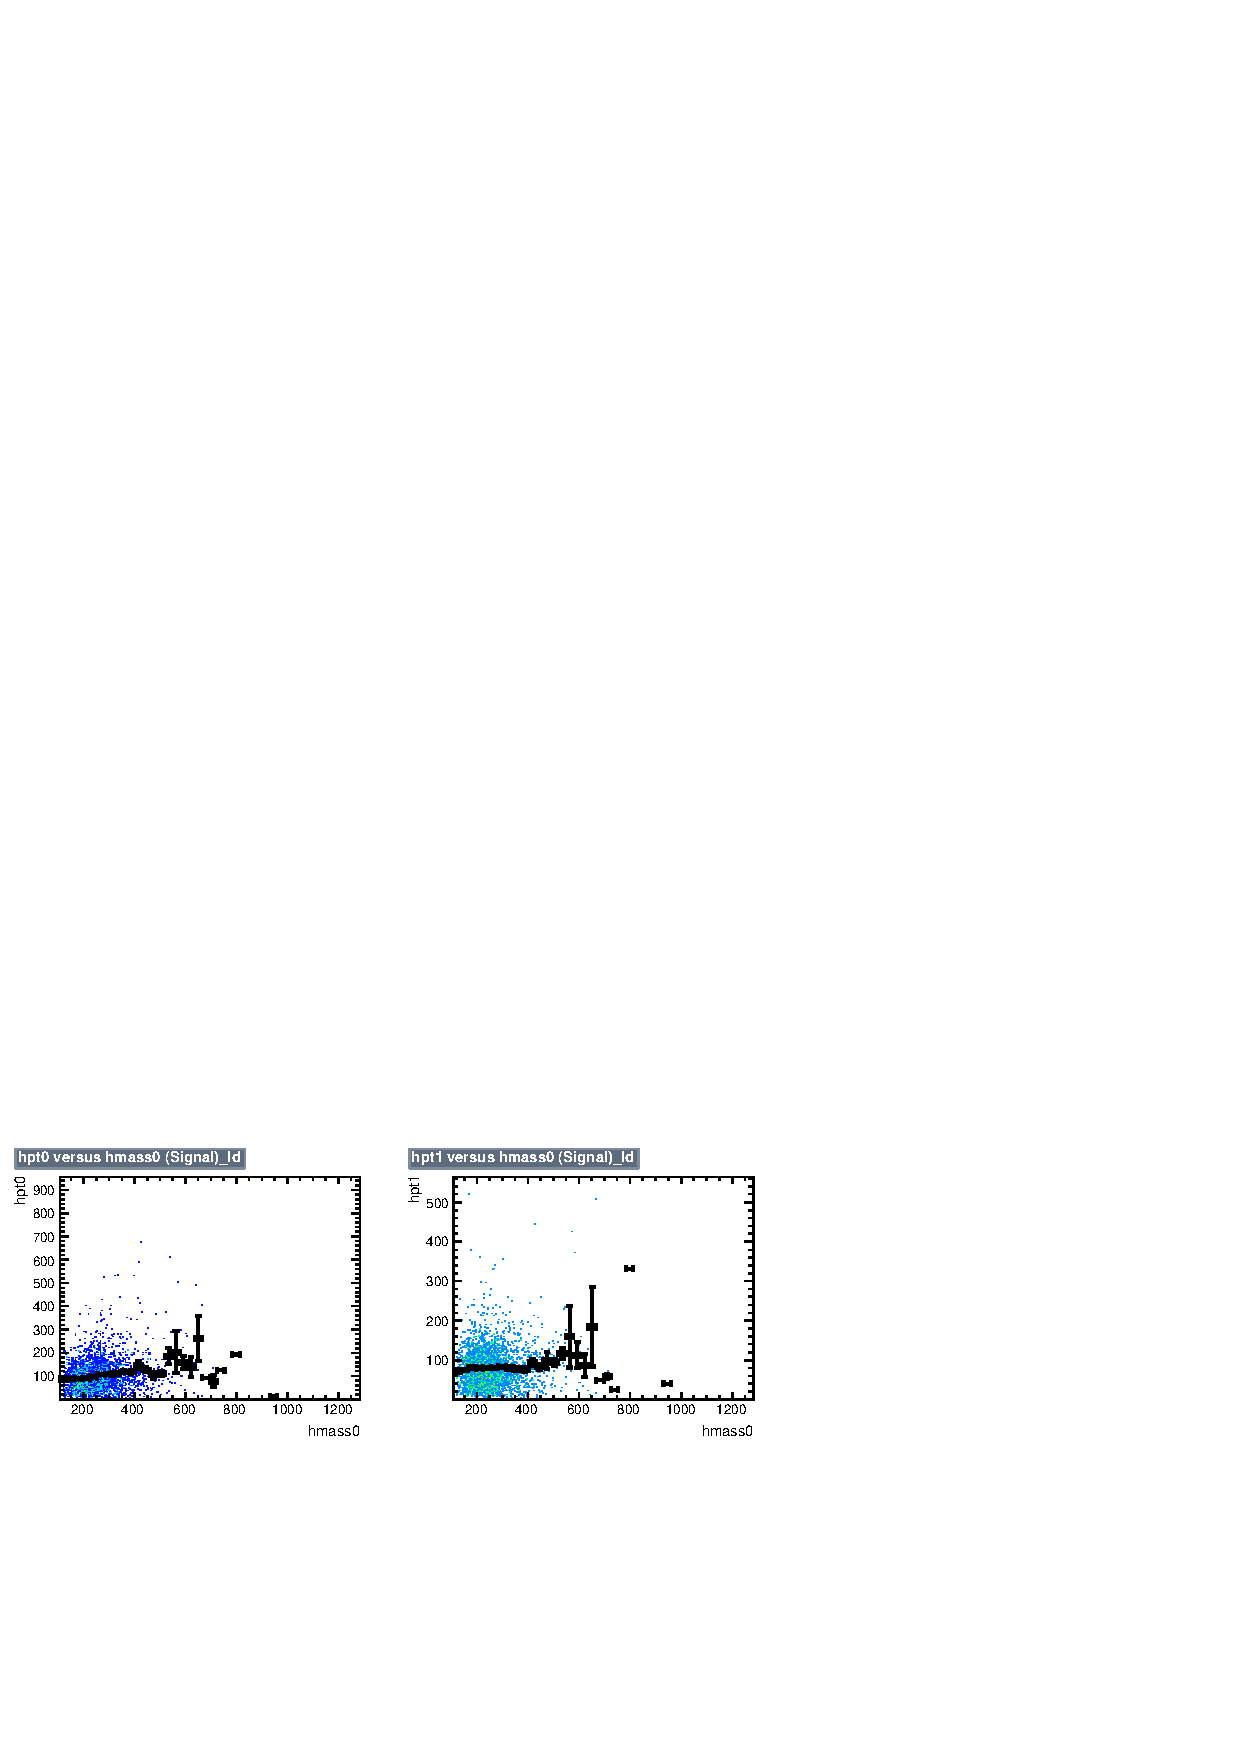
\includegraphics[width=0.95\textwidth]{figures/CRTT/dataset/plots/correlationscatter_hmass0__Id_c2.pdf}
\caption{ Correlation scatter plots for \HZZ mass  variable for data}%, index '1' refers to bb and index '0' refers to ZZ}
\label{fig:correlations_CRTT_hmass0_S}                                                       
\end{figure}



\begin{figure}[!htb]%hbpt?        
\centering
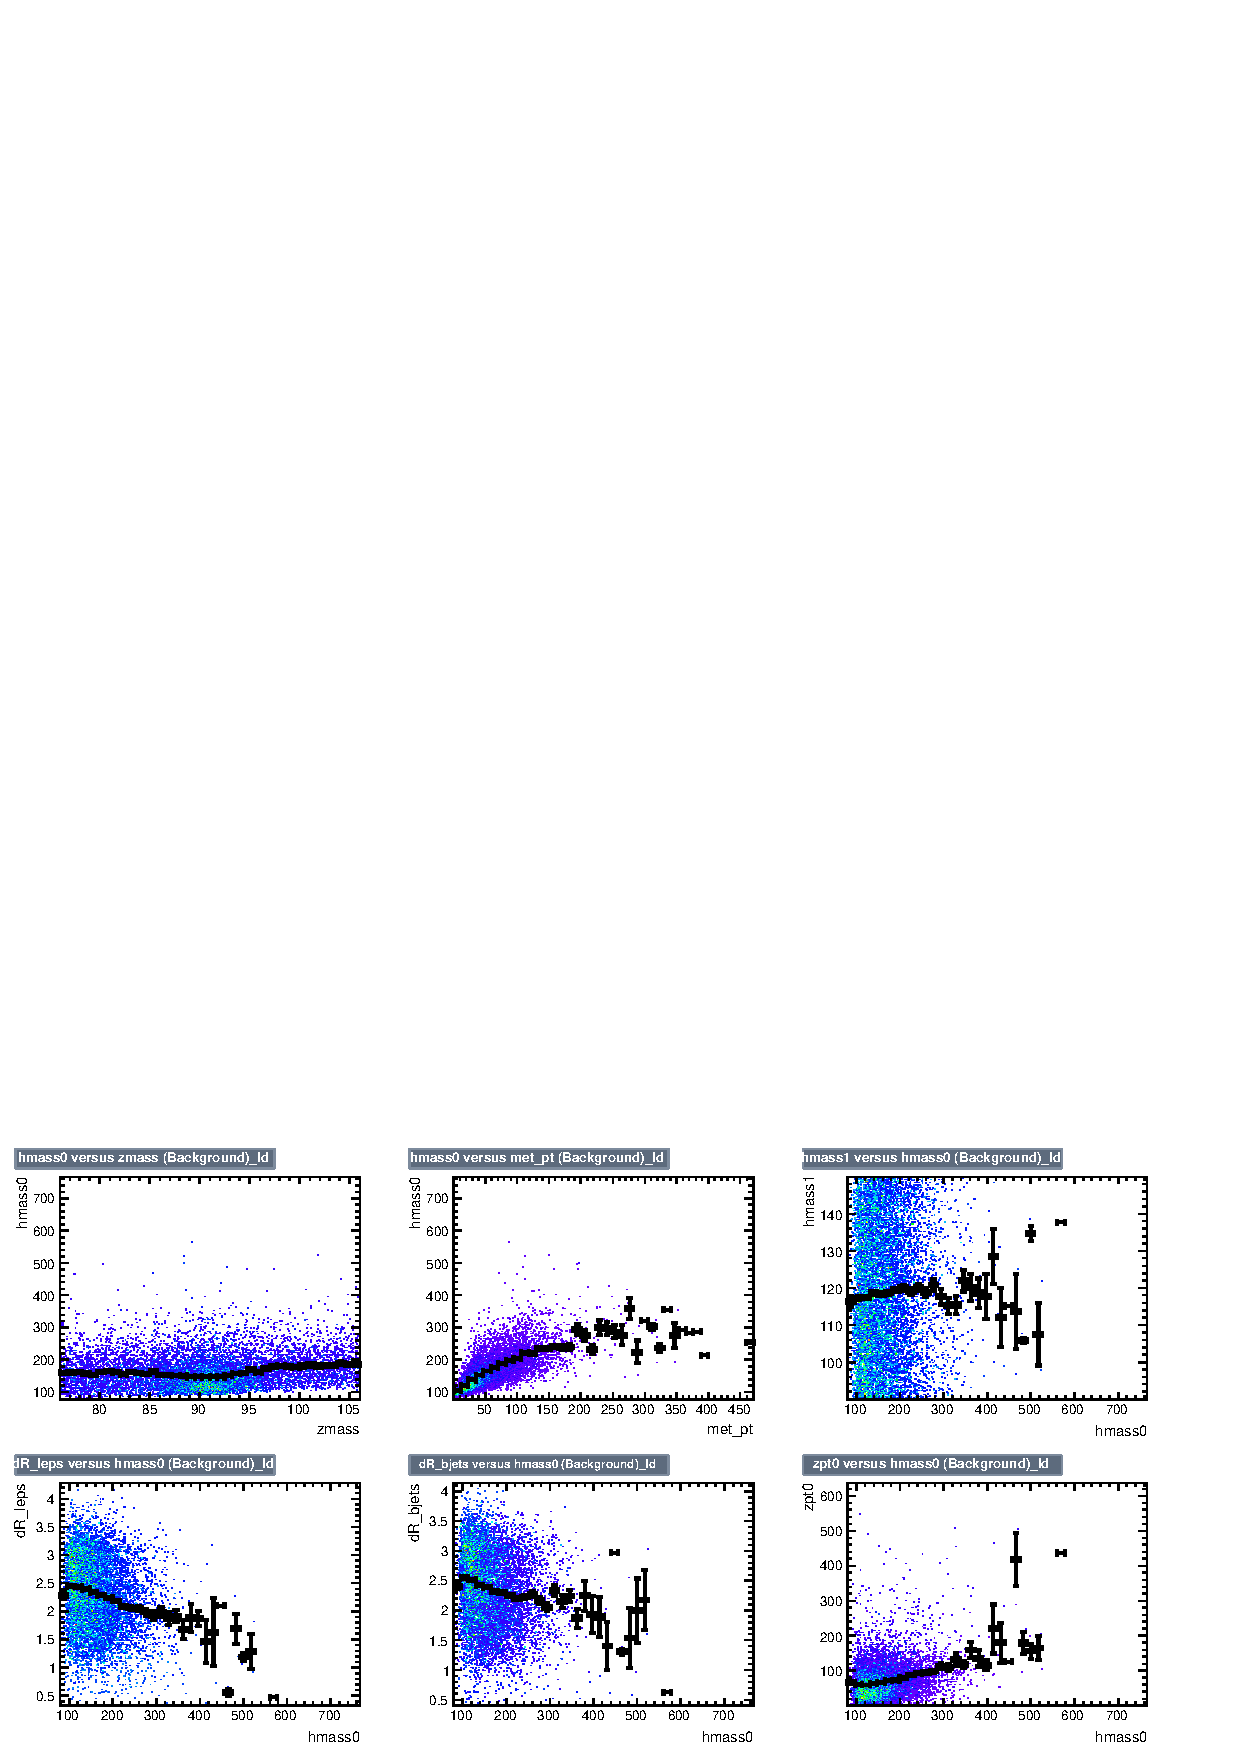
\includegraphics[width=0.95\textwidth]{figures/CRTT/dataset/plots/correlationscatter_hmass0__Id_c3.pdf}
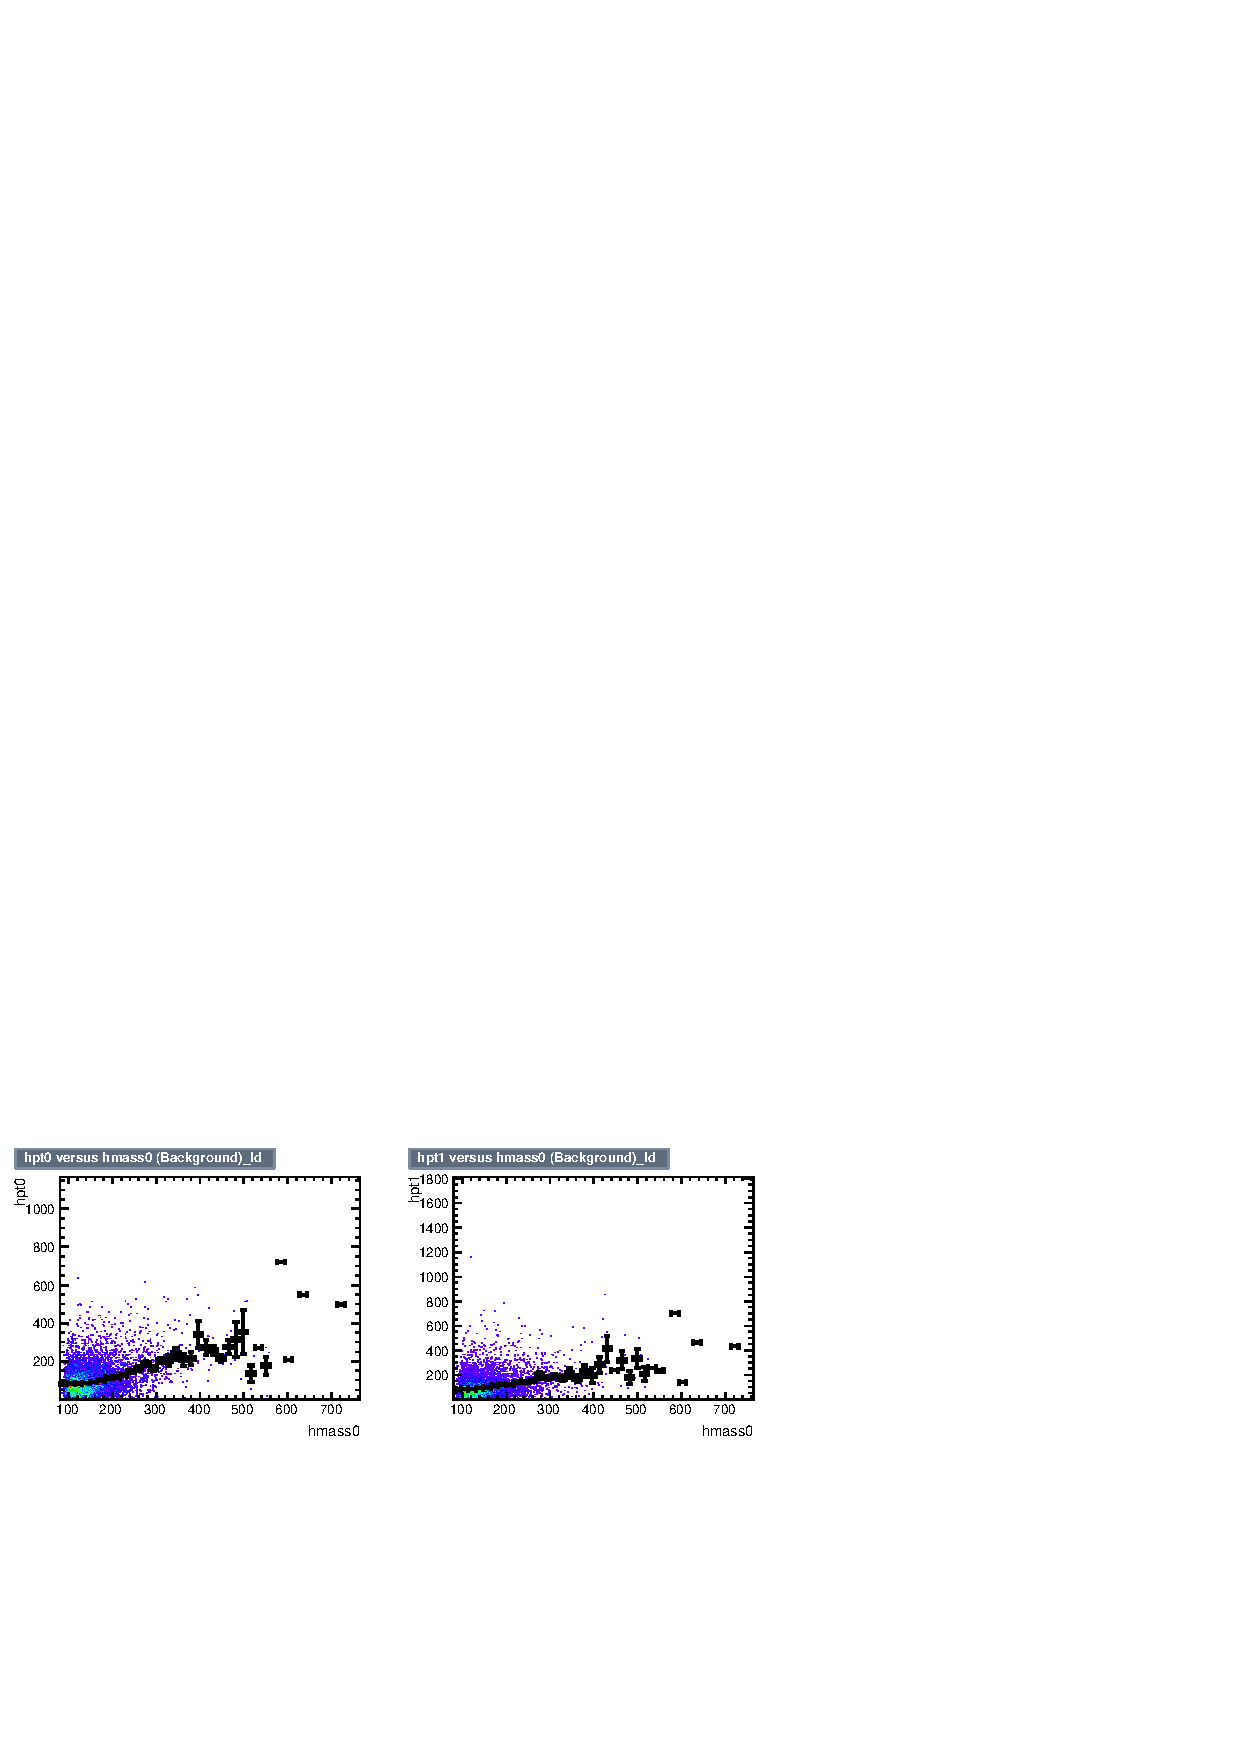
\includegraphics[width=0.95\textwidth]{figures/CRTT/dataset/plots/correlationscatter_hmass0__Id_c4.pdf}
\caption{ Correlation scatter plots for \HZZ mass variable for backgrounds}%, index '1' refers to bb and index '0' refers to ZZ}
\label{fig:correlations_CRTT_hmass0_BG}                                                       
\end{figure}




\begin{figure}[!htb]%hbpt?        
\centering
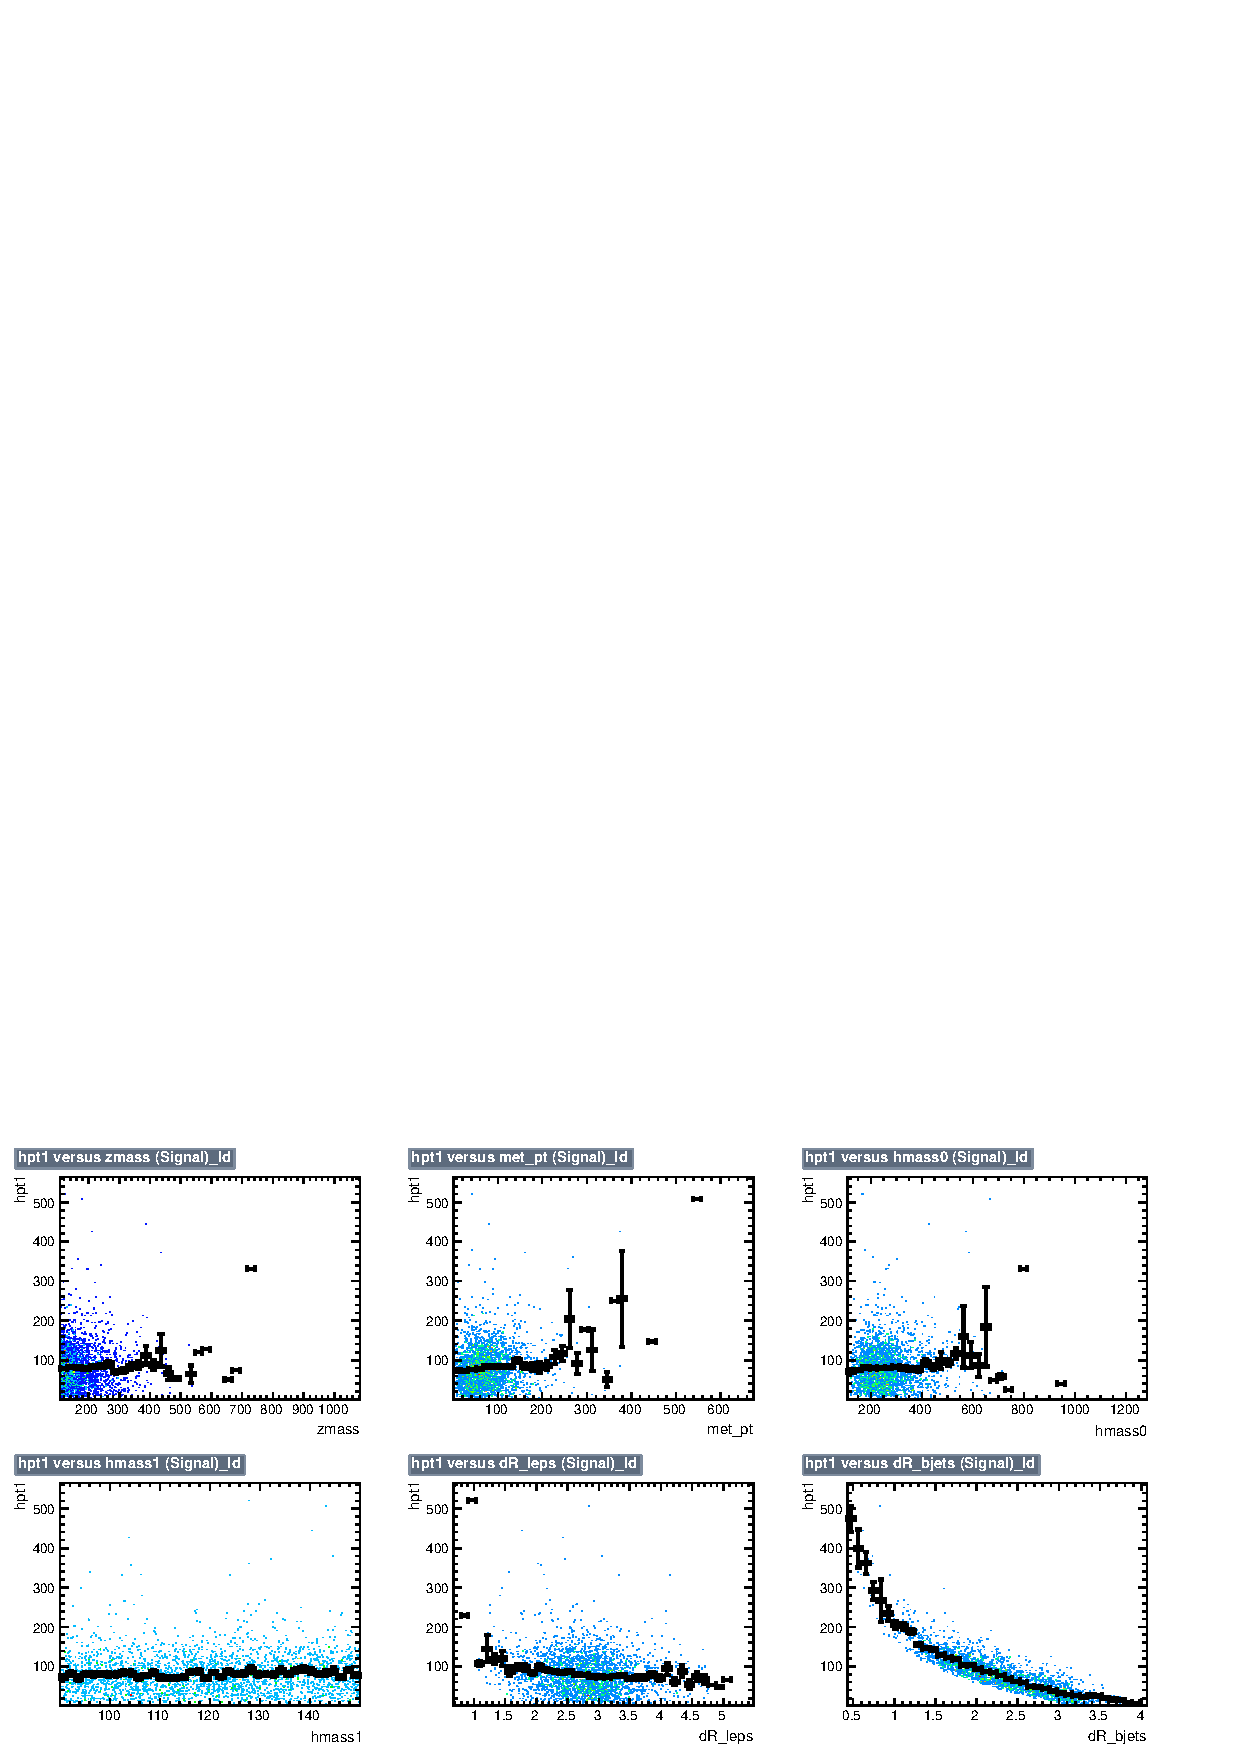
\includegraphics[width=0.95\textwidth]{figures/CRTT/dataset/plots/correlationscatter_hpt1__Id_c1.pdf}
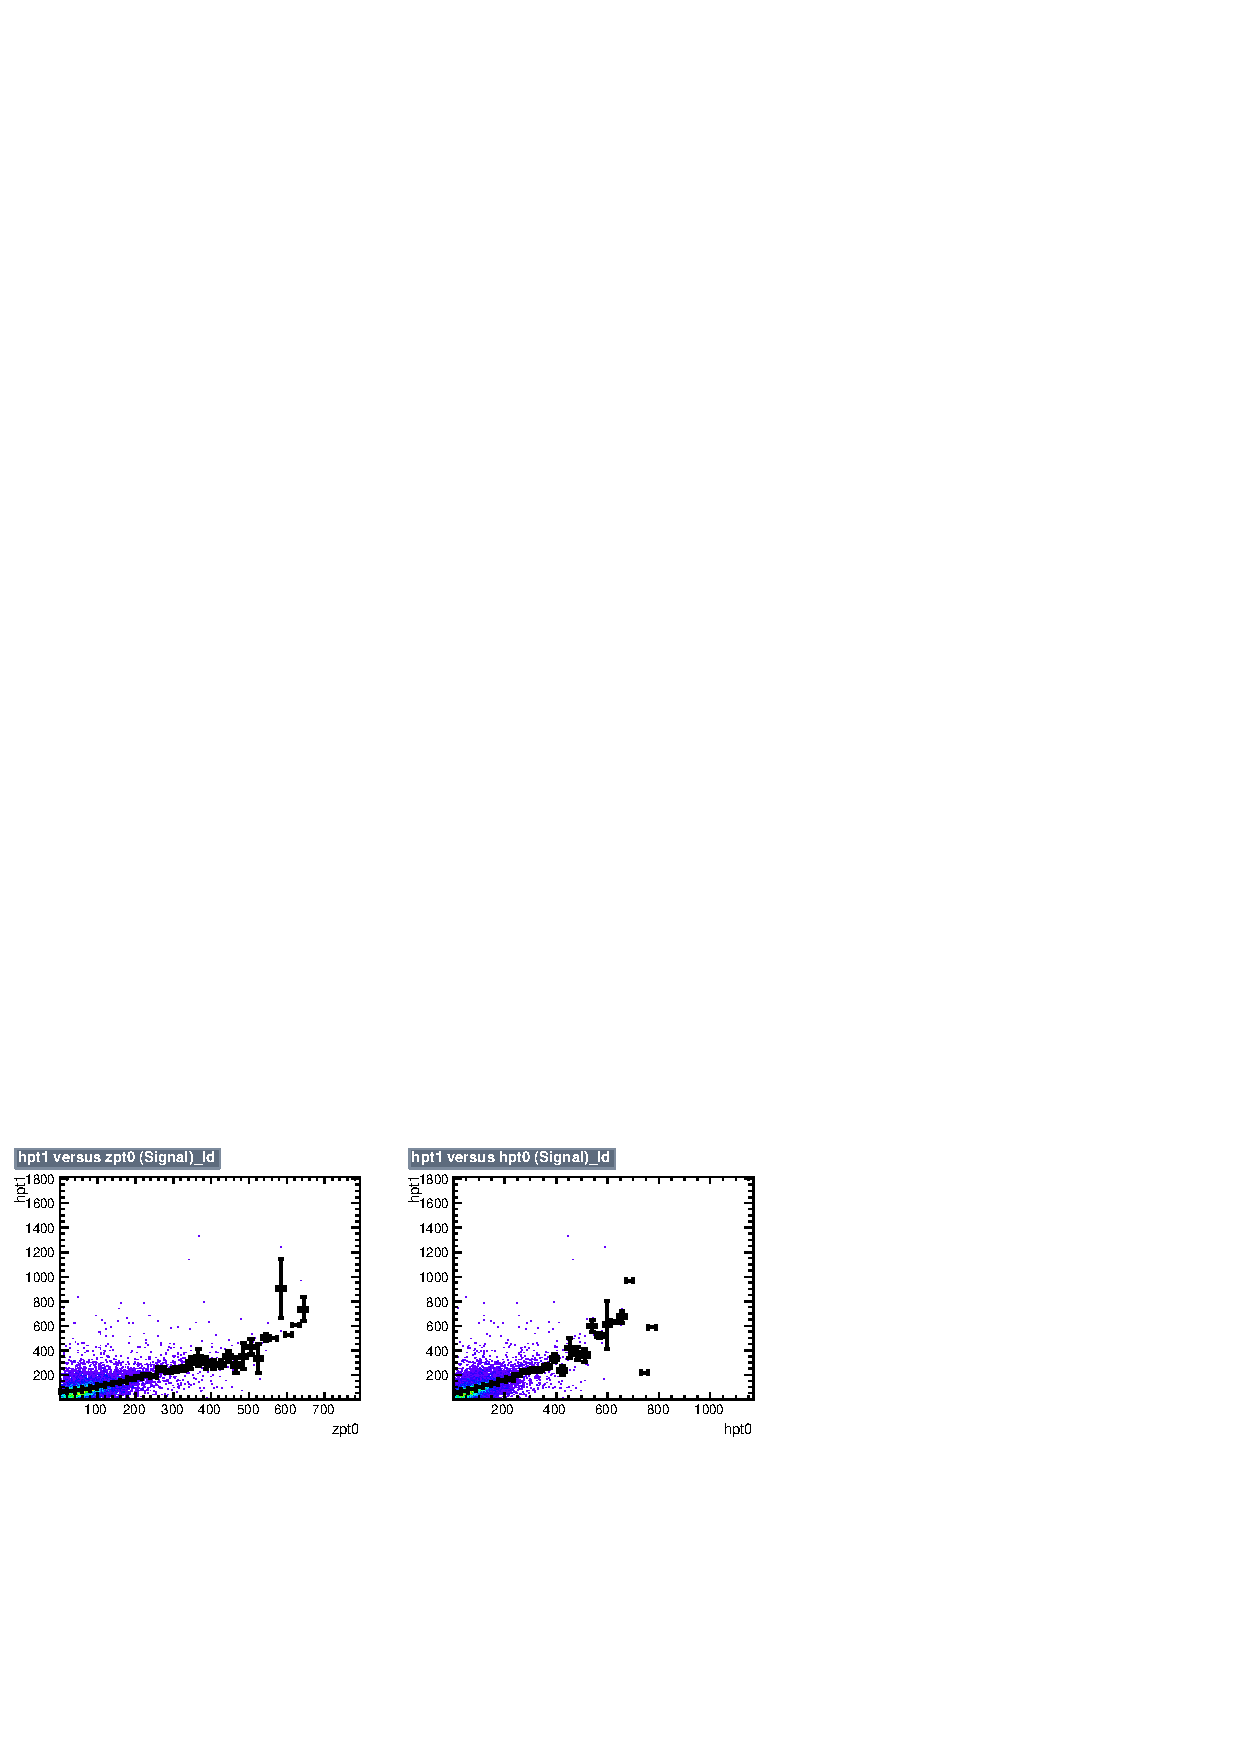
\includegraphics[width=0.95\textwidth]{figures/CRTT/dataset/plots/correlationscatter_hpt1__Id_c2.pdf}
\caption{ Correlation scatter plots for \HBB $p_{T}$  variable for data}%, index '1' refers to bb and index '0' refers to ZZ}
\label{fig:correlations_CRTT_hpt1_S}                                                       
\end{figure}



\begin{figure}[!htb]%hbpt?        
\centering
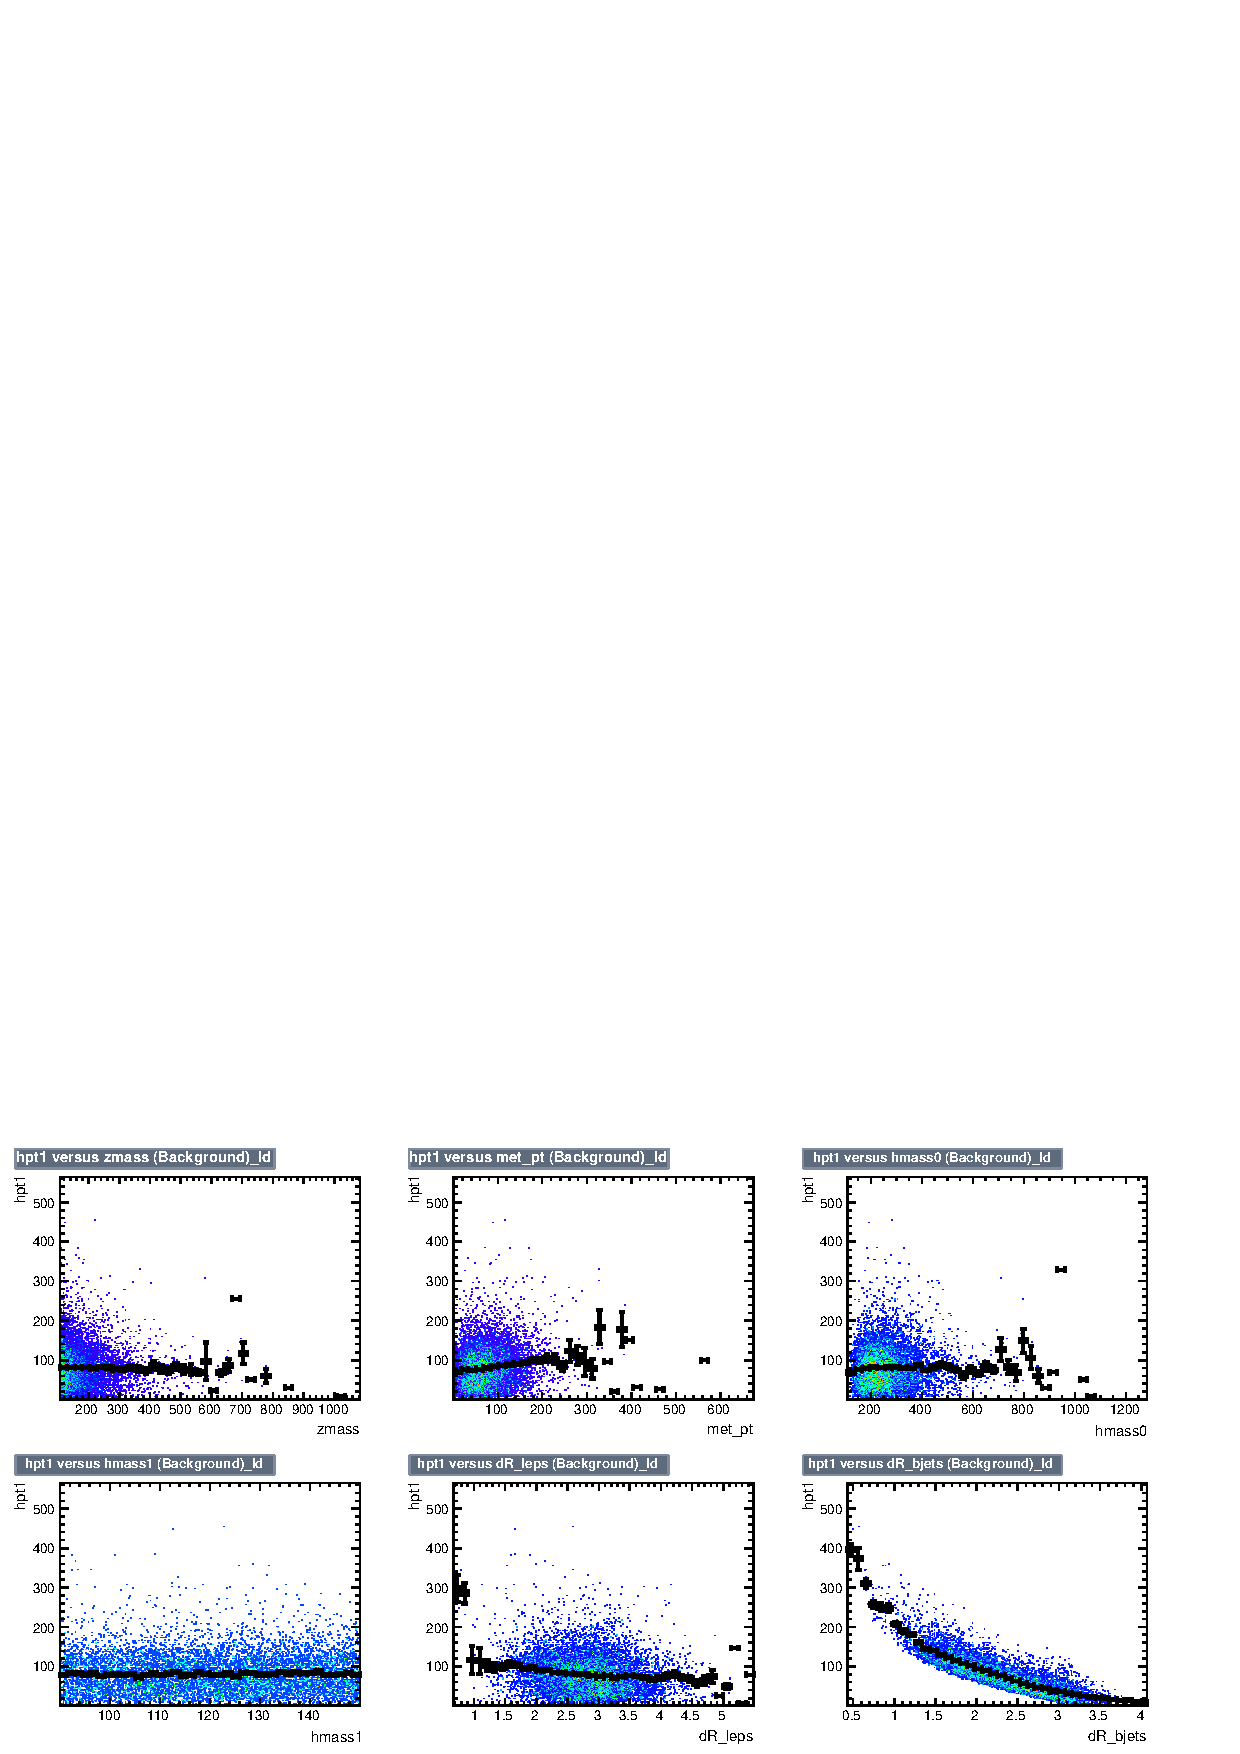
\includegraphics[width=0.95\textwidth]{figures/CRTT/dataset/plots/correlationscatter_hpt1__Id_c3.pdf}
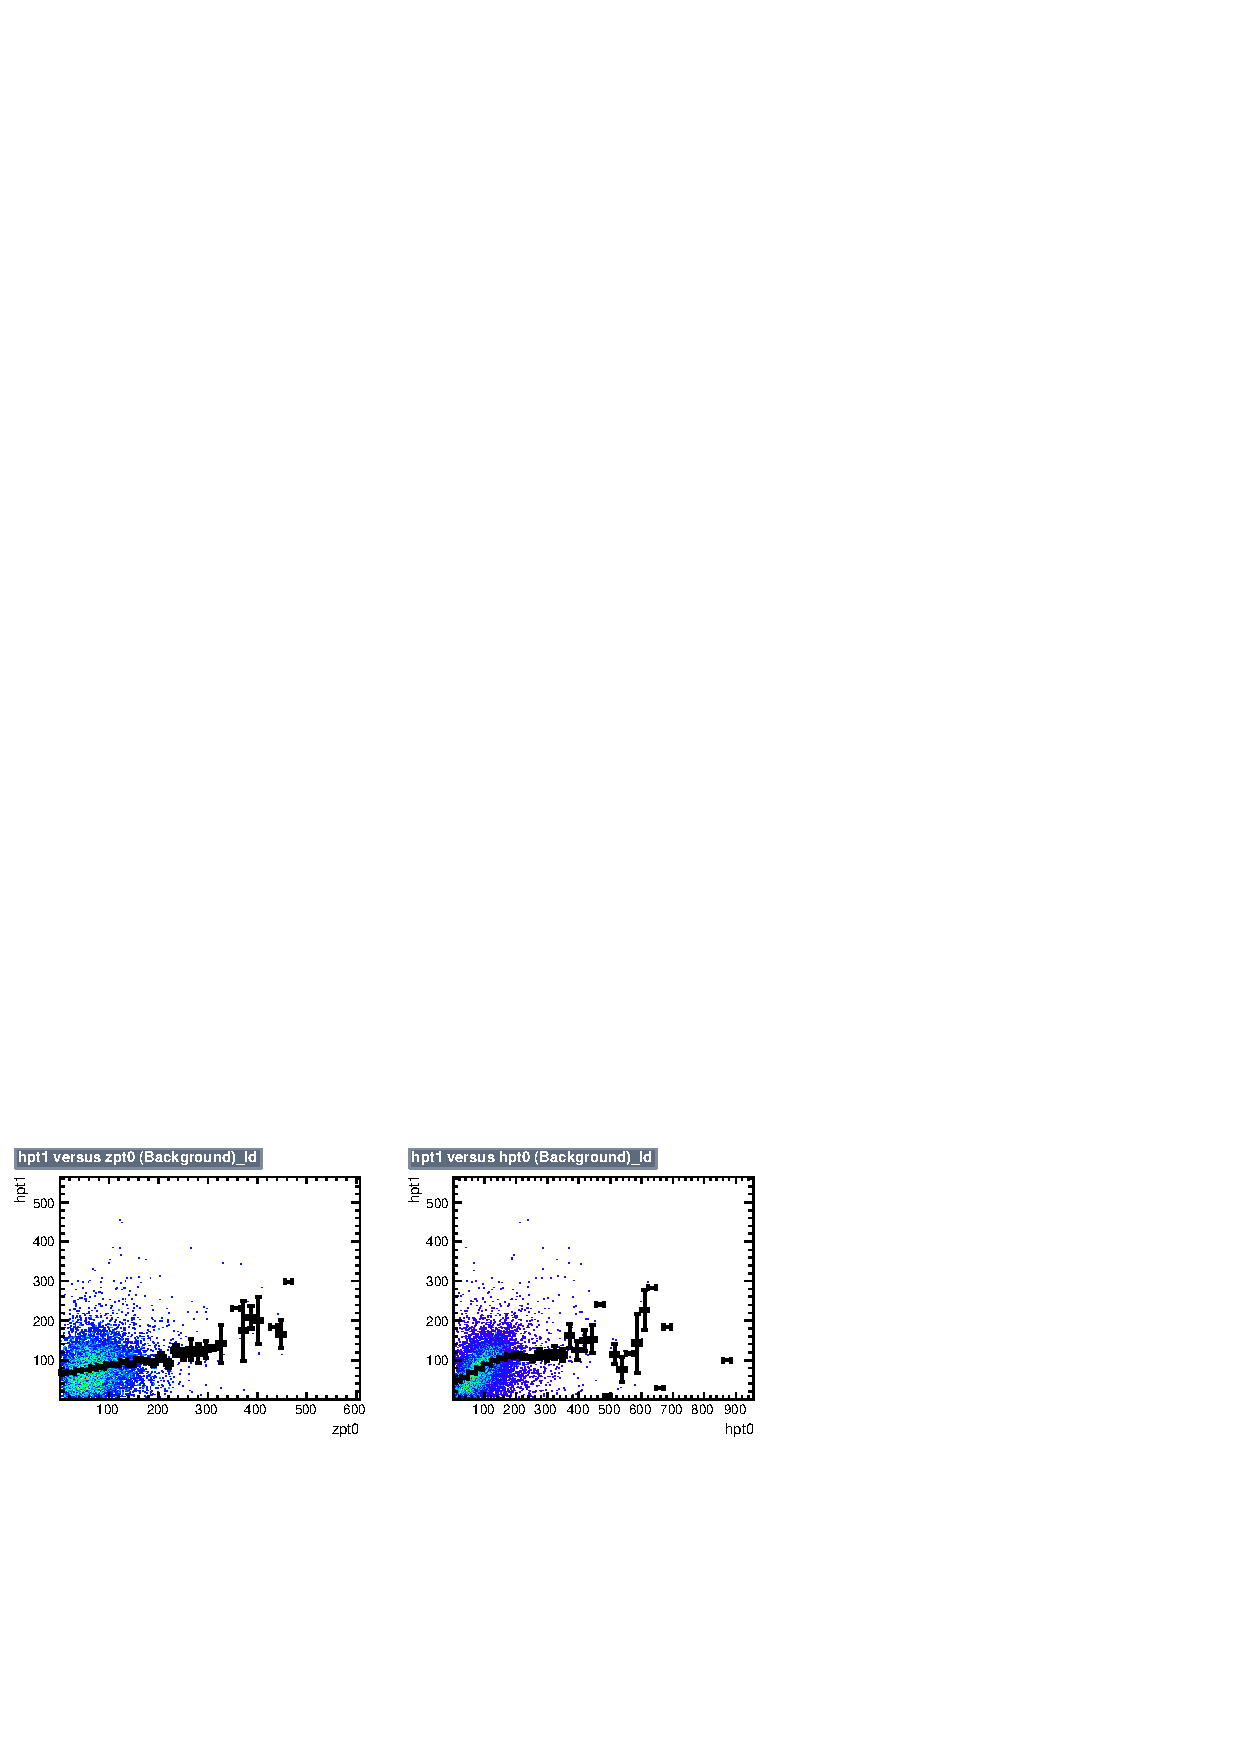
\includegraphics[width=0.95\textwidth]{figures/CRTT/dataset/plots/correlationscatter_hpt1__Id_c4.pdf}
\caption{ Correlation scatter plots for \HBB $p_{T}$ variable for backgrounds}%, index '1' refers to bb and index '0' refers to ZZ}
\label{fig:correlations_CRTT_hpt1_BG}                                                       
\end{figure}



\begin{figure}[!htb]%hbpt?        
\centering
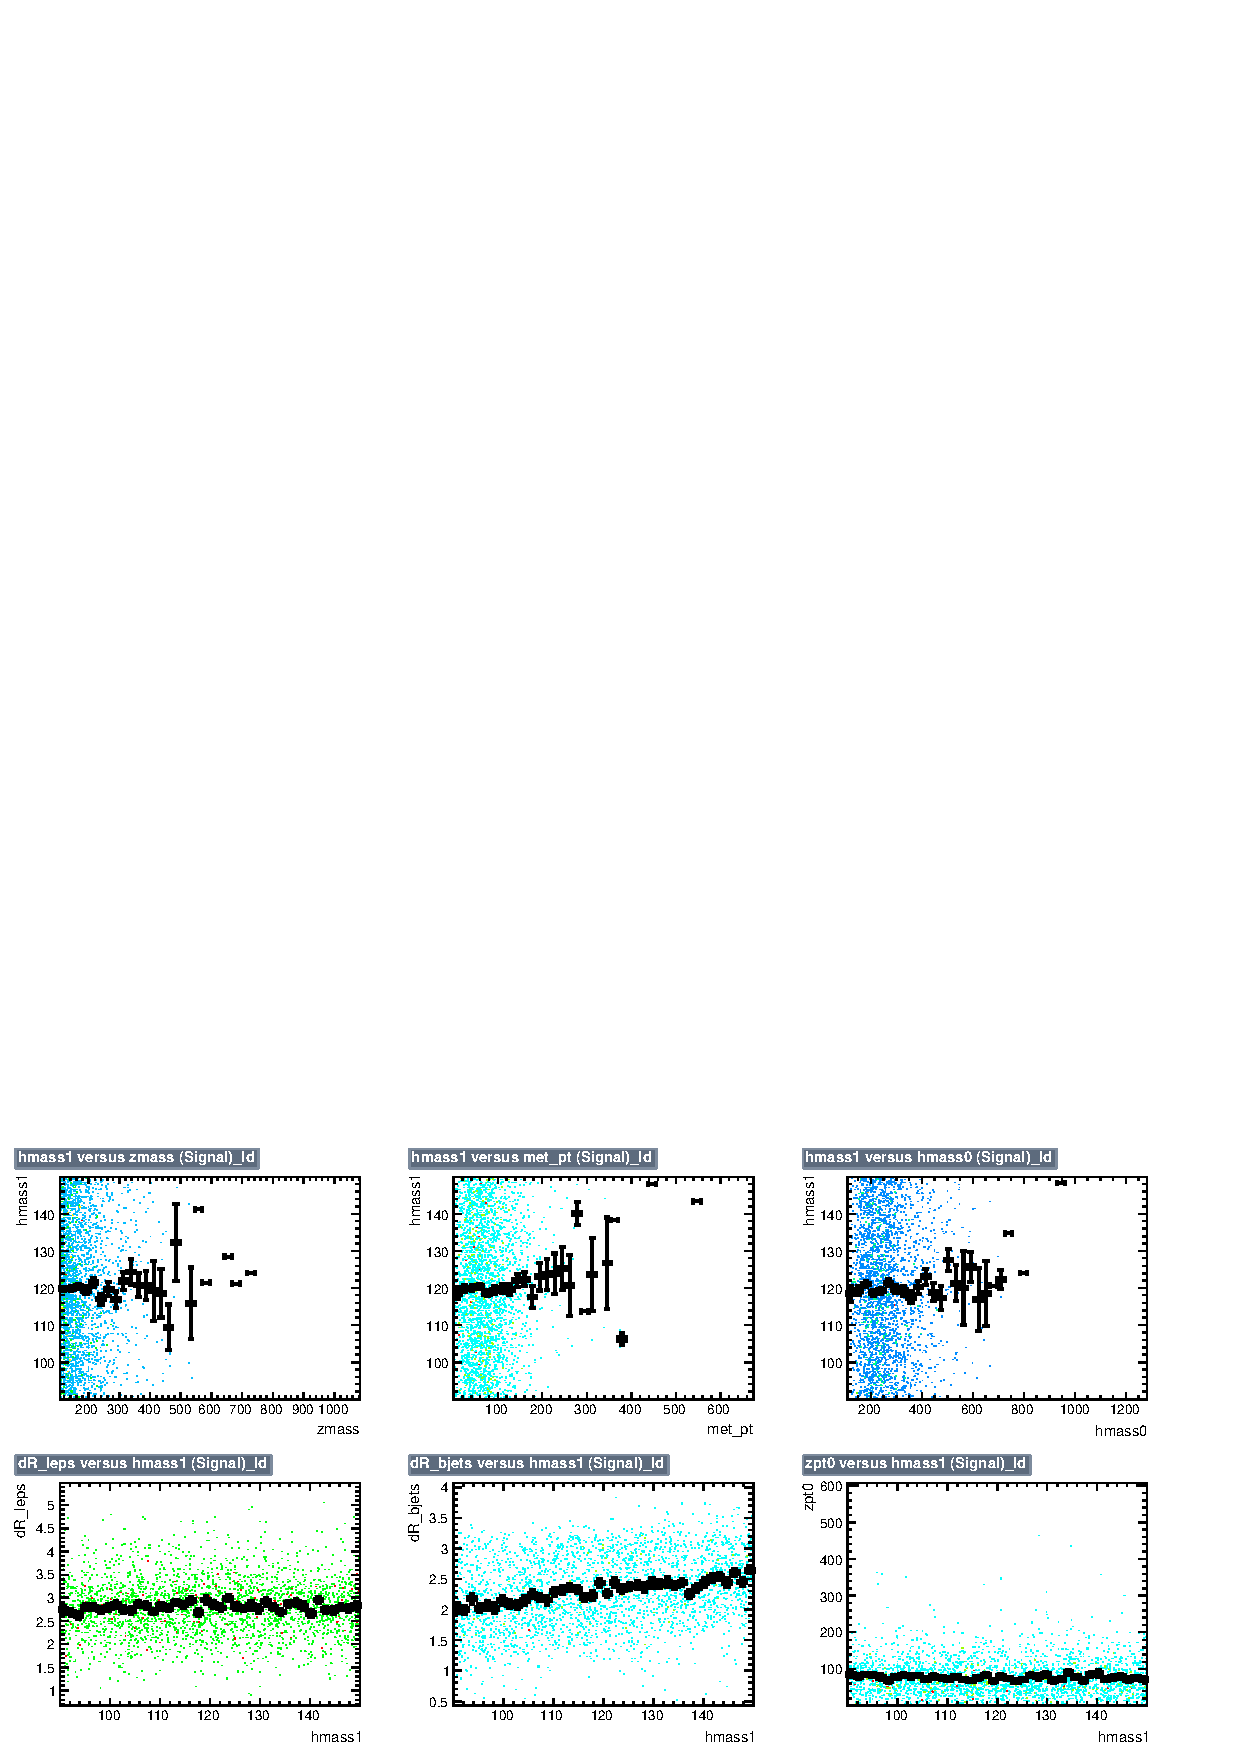
\includegraphics[width=0.95\textwidth]{figures/CRTT/dataset/plots/correlationscatter_hmass1__Id_c1.pdf}
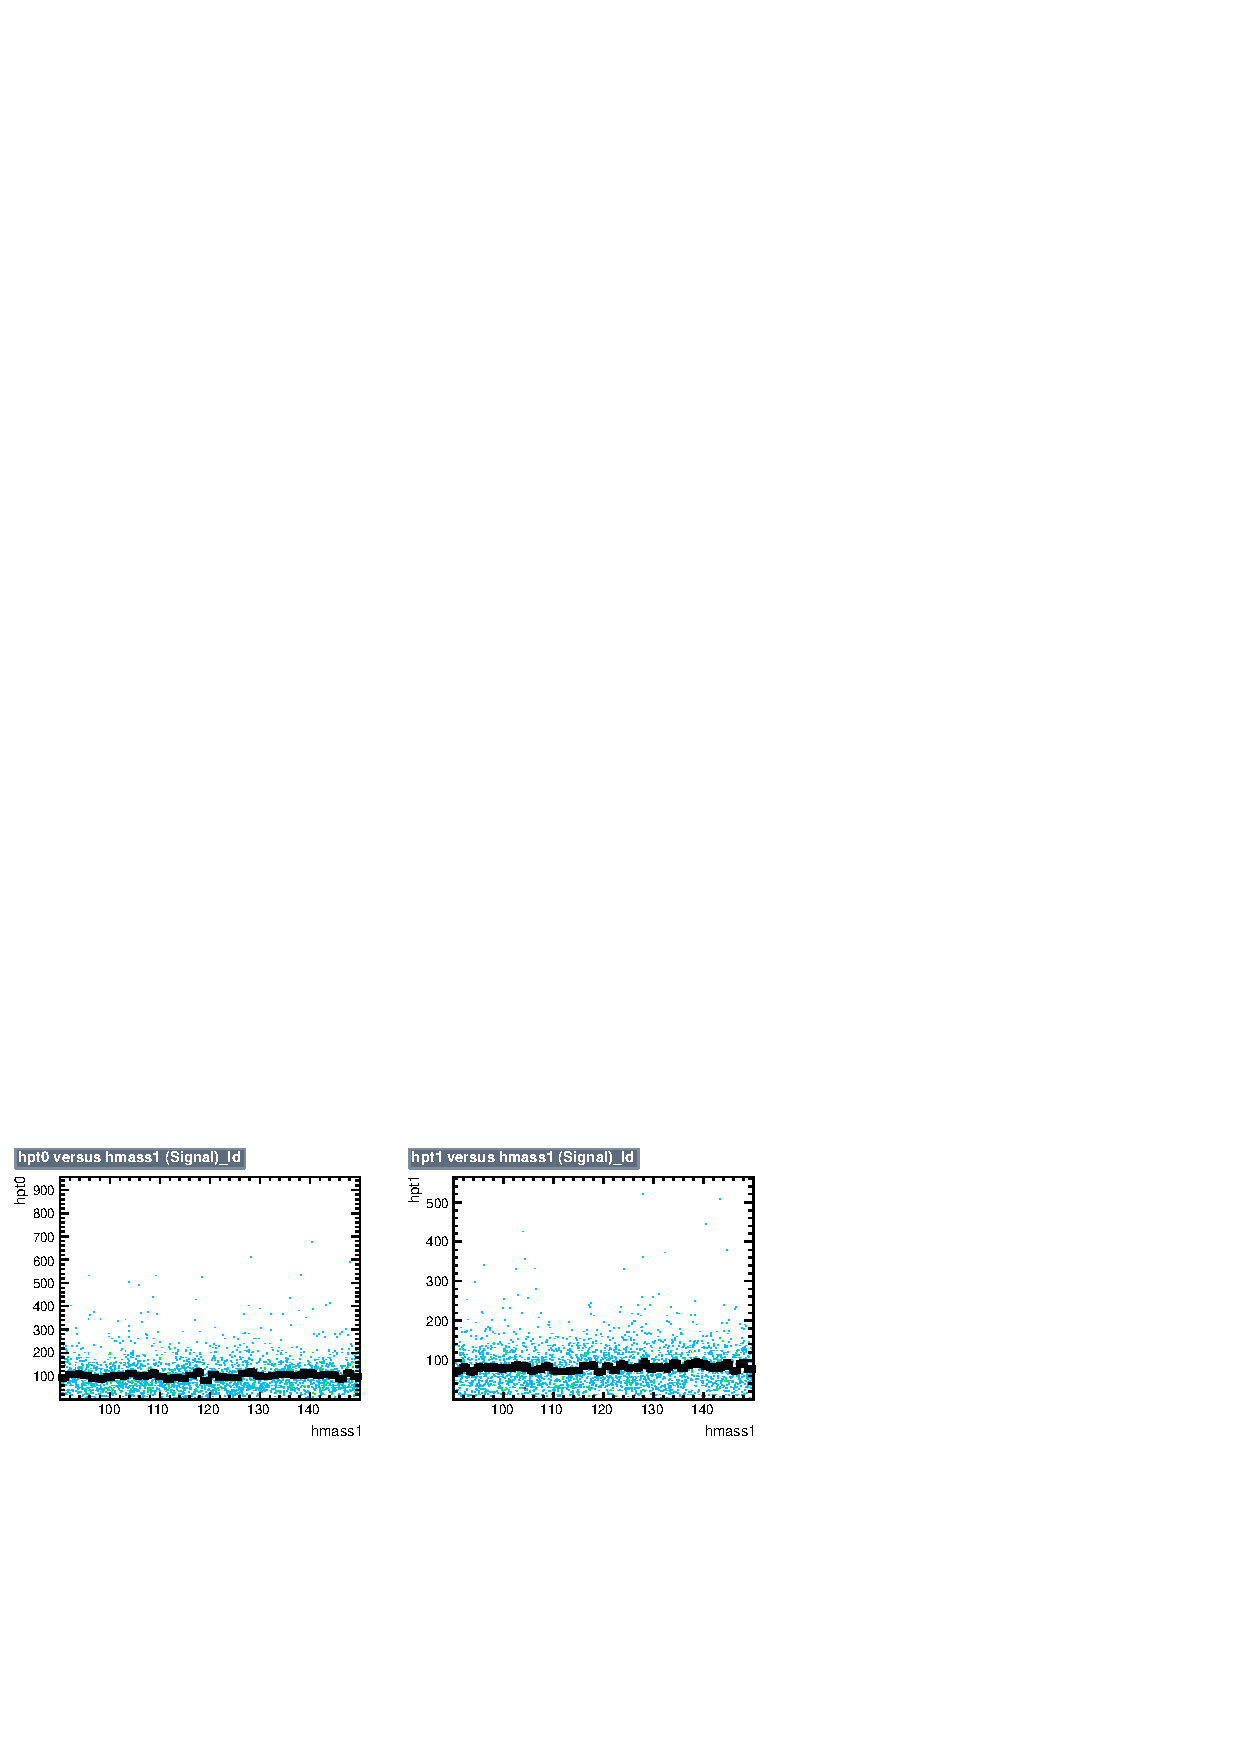
\includegraphics[width=0.95\textwidth]{figures/CRTT/dataset/plots/correlationscatter_hmass1__Id_c2.pdf}
\caption{ Correlation scatter plots for \HBB mass  variable for data}%, index '1' refers to bb and index '0' refers to ZZ}
\label{fig:correlations_CRTT_hmass1_S}                                                       
\end{figure}


%%%%%%    causes 
%! Undefined control sequence. \caption@ORI@xfloat ... \global \setbox \@currbox \color@vbox \normalcolor \... l.204 \begin{figure}[!htb]
\begin{figure}[!htb]%hbpt?        
\centering
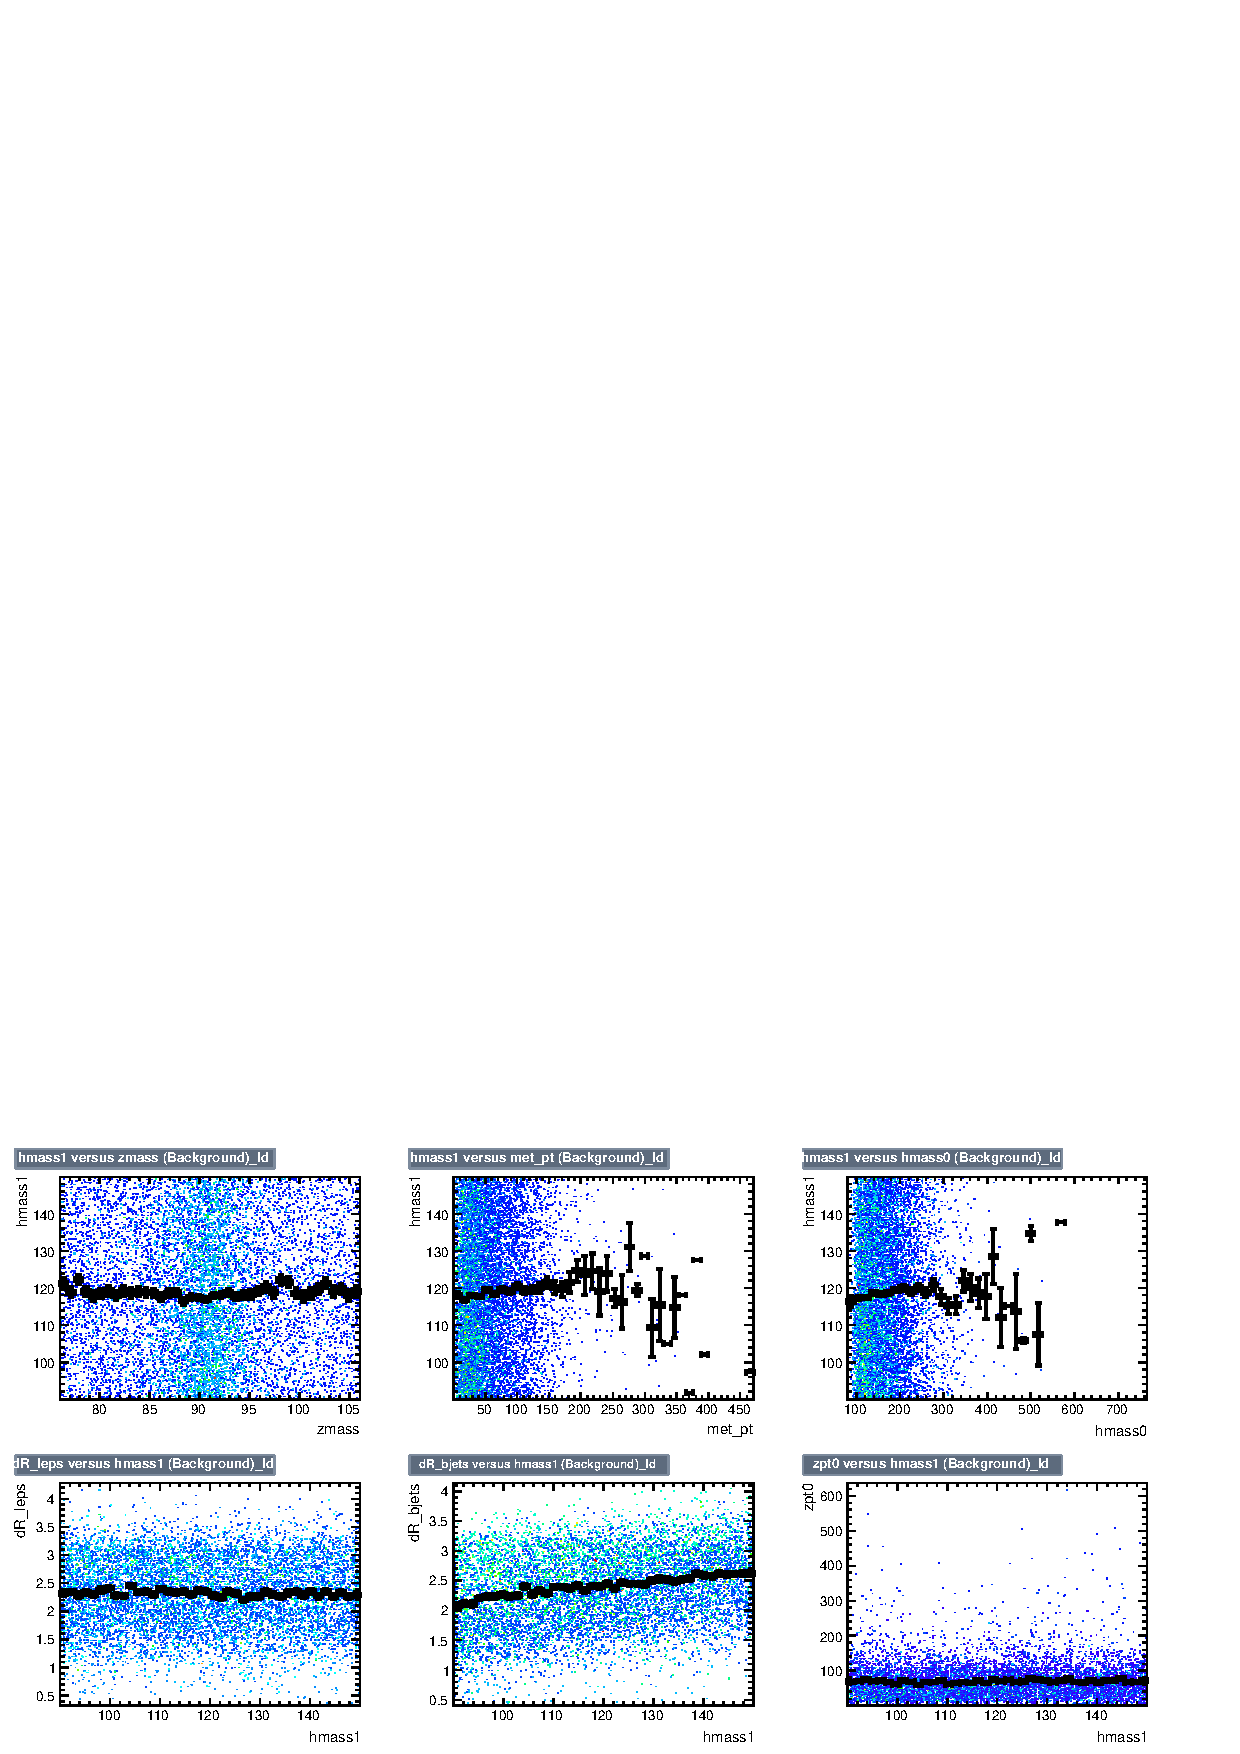
\includegraphics[width=0.95\textwidth]{figures/CRTT/dataset/plots/correlationscatter_hmass1__Id_c3.pdf}
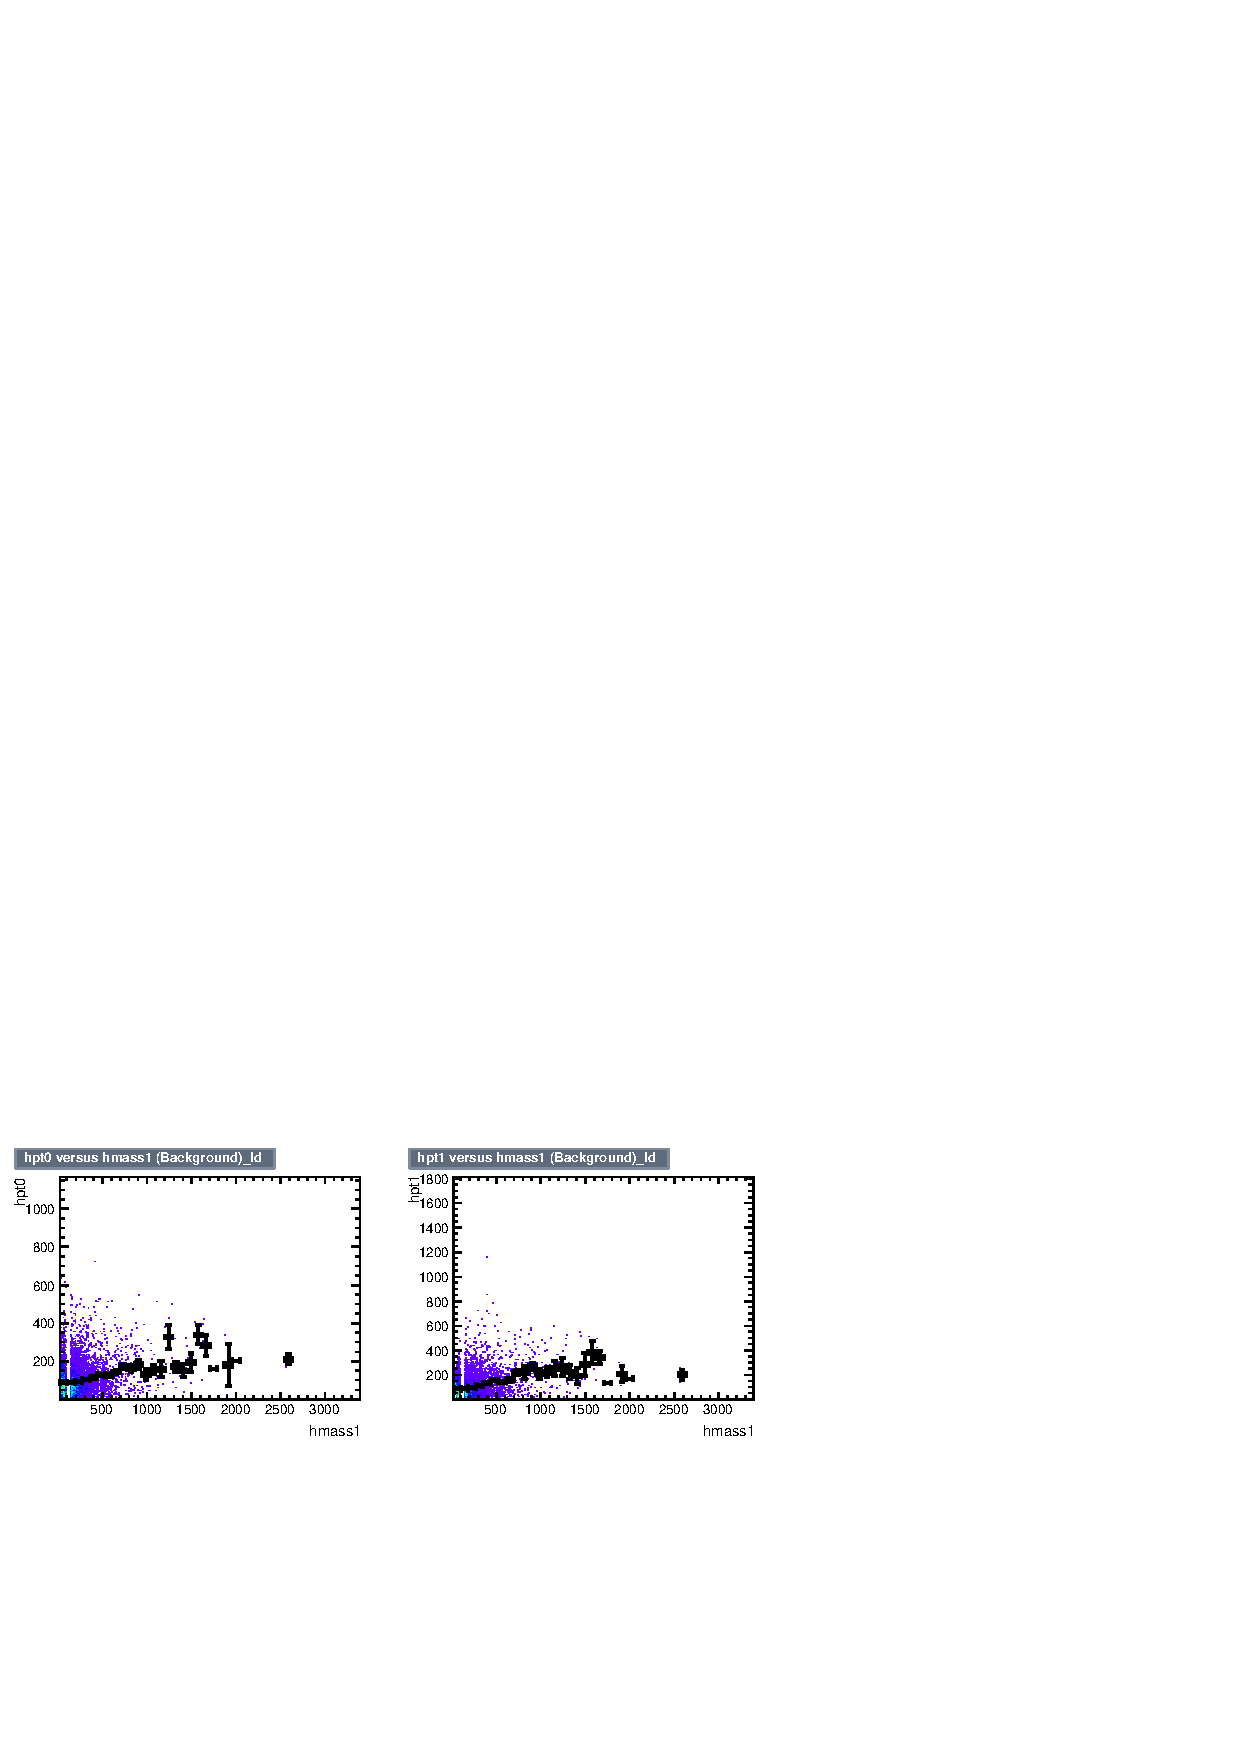
\includegraphics[width=0.95\textwidth]{figures/CRTT/dataset/plots/correlationscatter_hmass1__Id_c4.pdf}
\caption{ Correlation scatter plots for \HBB mass variable for backgrounds}%, index '1' refers to bb and index '0' refers to ZZ}
\label{fig:correlations_CRTT_hmass1_BG}                                                       
\end{figure}
 

